% This must be in the first 5 lines to tell arXiv to use pdfLaTeX, which is strongly recommended.
\pdfoutput=1
% In particular, the hyperref package requires pdfLaTeX in order to break URLs across lines.

\documentclass[11pt]{article}

% Remove the "review" option to generate the final version.
%\usepackage[review]{acl}
\usepackage[]{acl}

% Standard package includes
\usepackage{times}
\usepackage{latexsym}
\usepackage{natbib}
\usepackage{subcaption}

% For proper rendering and hyphenation of words containing Latin characters (including in bib files)
\usepackage[T1]{fontenc}
% For Vietnamese characters
% \usepackage[T5]{fontenc}
% See https://www.latex-project.org/help/documentation/encguide.pdf for other character sets

% This assumes your files are encoded as UTF8
\usepackage[utf8]{inputenc}

% This is not strictly necessary, and may be commented out,
% but it will improve the layout of the manuscript,
% and will typically save some space.
\usepackage{microtype}

% This is also not strictly necessary, and may be commented out.
% However, it will improve the aesthetics of text in
% the typewriter font.
\usepackage{inconsolata}

%\usepackage{url}            % simple URL typesetting
%\usepackage[hidelinks]{hyperref}       % hyperlinks
\usepackage{booktabs}       % professional-quality tables
\usepackage{amsfonts}       % blackboard math symbols
\usepackage{nicefrac}       % compact symbols for 1/2, etc.
\usepackage{enumitem}
\usepackage{multicol}
\usepackage{multirow}
\usepackage{array}
\usepackage{graphicx}
\usepackage{wrapfig}
\usepackage{latexsym}
\usepackage{amsmath}
\usepackage{listings}
\usepackage{mdframed}
\mdfsetup{nobreak=true}
\usepackage{xcolor}         % colors
% If the title and author information does not fit in the area allocated, uncomment the following
%
%\setlength\titlebox{<dim>}
%
% and set <dim> to something 5cm or larger.

%\usepackage[dvipsnames]{xcolor}
\interfootnotelinepenalty=10000 % to prevent footnote from splitting across pages: https://texfaq.org/FAQ-splitfoot

%%%%%%%%%%%%%%%%%%%%%%%%%%%%%%%%%%%
%%%%%% Appendix TOC %%%%%%%%%%%%

\usepackage{titletoc}

%\newcommand\letur{\textbf{LeTUR}}
\newcommand\ilpcsr{\texttt{\textbf{IL-PCSR}}}
\newcommand\coliee{\texttt{\textbf{COLIEE}}}
%\interfootnotelinepenalty=10000 % to prevent footnote from splitting across pages: https://texfaq.org/FAQ-splitfoot

\newcommand{\paul}[1]{\textcolor{red}{#1}$_{Paul}$}
\newcommand\AM[1]{\textbf{\textcolor{blue}{#1}$_{Ashutosh}$}}
\newcommand{\sg}[1]{\textcolor{magenta}{\textbf{[SG: #1]}}}
\newcommand\dg[1]{\textbf{\textcolor{cyan}{#1}$_{Dhananjay}$}}
\newcommand{\pg}[1]{\textcolor{purple}{\textbf{PG:} #1}}
\newenvironment{alltt}{\small\ttfamily}{\par}
% \newenvironment{smallredtext}{\small\color{red}}{\par}
\newcommand{\old}[1]{\textcolor{gray}{#1}$_{old}$}


\newcommand\TB[1]{\textcolor{blue}{#1}}


%\title{Instructions for *ACL Proceedings}
\title{IL-PCSR: Legal Corpus for Prior Case and Statute Retrieval}

%\title{IL-PCSR: Legal Prior Case and Statute Retrieval via an  Ensemble of Lexical and Deep Models}

% Author information can be set in various styles:
% For several authors from the same institution:
% \author{Author 1 \and ... \and Author n \\
%         Address line \\ ... \\ Address line}
% if the names do not fit well on one line use
%         Author 1 \\ {\bf Author 2} \\ ... \\ {\bf Author n} \\
% For authors from different institutions:
% \author{Author 1 \\ Address line \\  ... \\ Address line
%         \And  ... \And
%         Author n \\ Address line \\ ... \\ Address line}
% To start a separate ``row'' of authors use \AND, as in
% \author{Author 1 \\ Address line \\  ... \\ Address line
%         \AND
%         Author 2 \\ Address line \\ ... \\ Address line \And
%         Author 3 \\ Address line \\ ... \\ Address line}

% \author{First Author \\
%   Affiliation / Address line 1 \\
%   Affiliation / Address line 2 \\
%   Affiliation / Address line 3 \\
%   \texttt{email@domain} \\\And
%   Second Author \\
%   Affiliation / Address line 1 \\
%   Affiliation / Address line 2 \\
%   Affiliation / Address line 3 \\
%   \texttt{email@domain} \\}

\author{ {\bf Shounak Paul}$^\diamond$\thanks{\ Equal Contributions} \qquad
{\bf Dhananjay Ghumare}$^\mathparagraph$\footnotemark[1] \qquad \\
\textbf{Pawan Goyal}$^\diamond$ \qquad \textbf{Saptarshi Ghosh}$^\diamond$ \qquad {\bf Ashutosh Modi}$^\mathparagraph$\thanks{\ Corresponding Author}  
 \\ 
        $^\diamond$IIT Kharagpur \qquad
        $^\mathparagraph$IIT Kanpur\\
  %\texttt{shounakpaul95@kgpian.iitkgp.ac.in}, 
  \texttt{shounakpaul95@kgpian.iitkgp.ac.in}, \texttt{\{pawang,saptarshi\}@cse.iitkgp.ac.in}, \\
  \texttt{\{dhananjayg, ashutoshm\}@cse.iitk.ac.in},  
}


\begin{document}
\maketitle

% \input{ACL-RR-Feb/submission/sections/abstract}

% \input{ACL-RR-Feb/submission/sections/introduction}
% \input{ACL-RR-Feb/submission/sections/relatedwork}
% \input{ACL-RR-Feb/submission/sections/benchmark}
% \input{ACL-RR-Feb/submission/sections/experiments}
% \input{ACL-RR-Feb/submission/sections/conclusion}

\begin{abstract}
Identifying/retrieving relevant statutes and prior cases/precedents for a given legal situation are common tasks exercised by law practitioners. Researchers to date have addressed the two tasks independently, thus developing completely different datasets and models for each task; however, both retrieval tasks are inherently related, e.g., similar cases tend to cite similar statutes (due to similar factual situation). 
In this paper, we address this gap. We propose \ilpcsr{} (Indian Legal corpus for Prior Case and Statute Retrieval), which is a unique corpus that provides a common testbed for developing models for both the tasks (Statute Retrieval and Precedent Retrieval) that can exploit the dependence between the two. We experiment extensively with several baseline models on the tasks, including lexical models, semantic models and ensemble based on GNNs. Further, to exploit the dependence between the two tasks, we develop an LLM-based re-ranking approach that gives the best performance. 
\end{abstract}
% \begin{abstract}
% Identifying relevant statutes and prior cases/precedents for a given legal case are two of the most common tasks exercised by legal practitioners. Researchers till date have addressed the two tasks independently, thus developing completely different datasets and models for each of the task, making it difficult to compare models across both tasks despite both being legal document retrieval problems. Given the paucity of such corpora, in this resource paper, we propose a new corpus \ilpcsr{} (Indian Legal corpus for Prior Case and Statute Retrieval), which is a unique corpus that provides a common testbed for developing models for both the tasks (Statue Retrieval and Precedent Retrieval). We experiment extensively with several baseline models on the tasks, including lexical models and semantic models. Results show that the ensemble of a semantic model (GNN) and a lexical model (BM25) gives the best performance.
% \end{abstract}
% Identifying relevant statutes and prior precedents for a given legal case are two of the most common tasks exercised by legal practitioners. Given the quantum of legal cases in modern times, these tasks need to be automated in order to expedite the legal workflow. Researchers till date have addressed the two tasks independently. However, there is a strong correlation between precedents and statues cited in a legal case; hence it makes sense to model both the tasks jointly. Given the paucity of such corpora, in this resource paper, we propose a new corpus IL-PCSR (Indian Legal corpus for Prior Case and Statute Retrieval), which is the first corpus for doing the two tasks (Statue Retrieval and Precedent Retrieval) together. 
% We experiment extensively with several baseline models on the tasks. We propose a new model based on ensemble of a GNN-based architecture and BM-25 for both the tasks. Results show that the ensemble of a semantic model (GNN) and a lexical model (BM-25) gives the best performance on both the tasks.

% Identifying relevant statutes and prior prece-001
% dents for a given legal case are two of the most002
% common tasks exercised by legal practitioners.003
% Given the quantum of legal cases in modern004
% times, these tasks need to be automated in or-005
% der to expedite the legal workflow. Researchers006
% till date have addressed the two tasks indepen-007
% dently. However, there is a strong correlation008
% between a case and its precedents and statutes009
% invoked in both; hence it makes sense to model010
% both the tasks jointly. Given the paucity of such011
% corpora, in this resource paper, we propose a012
% new corpus IL-PCSR (Indian Legal corpus for013
% Prior Case and Statute Retrieval), which is the014
% first corpus for doing the two tasks (Statue Re-015
% trieval and Precedent Retrieval) together. We016
% experiment extensively with several baseline017
% models on the tasks. We propose a new model018
% based on ensemble of a GNN-based architec-019
% ture and BM-25 for both the tasks. Results020
% show that the ensemble of a semantic model021
% (GNN) and a lexical model (BM-25) gives the022
% best performance on both the tasks.

%\vspace{-3mm}
\section{Introduction} \label{sec:introduction}
%\vspace{-3mm}

% \sg{
% Start directly saying that in Legal Analytics especially in Common Law countries, there are two practical and popular tasks - given a legal case, identify relevant statutes and precedents (prior cases). \\
% There have been many works on both tasks, but every prior work has focused on only one task. In reality, Law practitioners often have to do both tasks together. But till date, there is even no dataset that enables development of models for doing both tasks together. The objective of this work is to bridge this gap. \\
% We develop the first dataset for ... Describe the dataset we develop briefly (point to the dataset comparison table).\\
% We benchmark a wide variety of methods on the dataset ... state some methods.\\
% This first-of-its-kind dataset and analyses bring out some surprising observations - lexical methods perform well in one task while semantic methods perform well in the other. A probable reason for this surprising observation is the difference in the nature of the two tasks (explain). For this reason, multi-tasking approaches also do not achieve much improvement.\\
% Finally we develop simple ensemble approaches that combine the two types of methods, and successfully achieve improvements over both tasks.\\
% We also perform experiments over datasets from other legal jurisdictions and verify that the ensemble approaches achieve improvement. \\
% End with a recap of our main contributions.
% }\paul{Addressed}
%These can be time consuming activities and may suffer from recall issues. 

\noindent In the legal domain, laws (statutes) and prior cases are considered to be the fundamental sources of knowledge that guide principles of jurisdiction~\cite{joshi2023ucreat}. 
In practice, a legal practitioner when faced with a legal case, typically uses their experience and knowledge to identify prior precedents and applicable statutes in the given situation. 
This process is time-consuming, and the problem worsens with the growing number of legal cases in populous countries like India \cite{malik2021ildc}. Hence, there is an imminent need to automate the process to make it more efficient. 

% \noindent Two tasks have been proposed independently in this regard: Legal Statute Retrieval (LSR) -- that aims to identify/retrieve statutes that are applicable in a given query case \cite{paul2024legal}, and Prior Case Retrieval (PCR) -- that aims to identify/retrieve relevant prior cases/precedents that should be cited by the given query case \cite{joshi2023ucreat}. Traditionally, the two tasks have been modeled separately leading to creation of different corpora and models for each of them. However, both the tasks are inherently related. For example, a legal case would typically cite another prior legal case if they share similar factual situation, consequently both would be citing similar statutes. For computational models to exploit such relationships a corpus which combines both the tasks is required. We address this gap by making following contributions:

\noindent Two tasks have been proposed independently in this regard: Legal Statute Retrieval (LSR) -- that aims to identify/retrieve statutes that are applicable in a given query case \cite{paul2024legal}, and Prior Case Retrieval (PCR) -- that aims to identify/retrieve relevant prior cases/precedents that should be cited by the given query case \cite{joshi2023ucreat}. Traditionally, the two tasks have been modeled separately leading to creation of different corpora and models for each of them. However, both tasks are inherently connected in real legal practice. In India, as well as in many other countries, case law is treated as a primary source of law supplementing statutes, regulations, and constitutional provisions~\citep{manupatra-guide}. 
%and official legal infrastructures such as the India Code Information System (ICIS: \url{https://www.indiacode.nic.in}) provides mechanisms to locate the relevant precedents and amendments while retrieving statutes.
For example, a legal case would typically cite another prior legal case if they share similar factual situation, and consequently both would be citing similar statutes. For computational models to exploit such connections, a corpus which combines both the tasks is required. We address this gap by making the following contributions:



%It makes it difficult to compare models across tasks, since the models were not aware in any way about the other task during training. \paul{However, both the tasks are essentially legal document retrieval tasks, hence it would be interesting to explore if it is possible to utilize the outputs/training gained by one task in a bid to improve the other.} This requires a common corpus for both the tasks having query cases (with missing precedent citations and missing statutes) and corresponding pool of candidate prior cases and pool of candidate statutes. We address this gap in this paper. In a nutshell, we make the following contributions:
%statues and prior precedents are correlated. For example, a case citing a prior precedent is likely to share similar factual situation and consequently both the cases are likely to invoke similar statues. In this work, explore the possibility of modeling both the tasks simultaneously. However, for solving both the tasks together there is a lack of any corpus having query cases (with missing precedent citations and missing statutes) and corresponding pool of candidate prior cases and pool of candidate statutes. In this scenario, we make the following contributions:
\begin{itemize}[noitemsep,nosep,leftmargin=*]
\item  In this paper, we propose \ilpcsr\ (Indian Legal Corpus for Prior Case and Statute Retrieval), a large corpus of query cases along with a candidate pool of prior cases and statutes in English for the Indian legal domain. To the best of our knowledge, we are first to develop such a corpus having both prior cases and statutes for the same set of queries. 
\item We perform extensive experiments with a variety of models for  each task, including lexical models (e.g., BM-25) and semantic models (e.g., transformer-based models and GNNs). Further, we experiment with an ensemble of semantic and lexical models, which improves performance in both tasks.
%\paul{Finally, we develop a prompting-based technique with an LLM to re-rank the top candidates given by the ensemble model.}
\item To test our intuition about inherent dependencies between the two tasks, we develop two methods: 
(i)~joint prediction model for both tasks via multi-task learning model based on GNNs; 
(ii)~a unique pipeline based approach comprising of an ensemble model that acts as a retriever, and an LLM as a re-ranker that performs tasks in a sequential order. The pipeline-based approach (in either order LSR $\rightarrow$ PCR or PCR $\rightarrow$ LSR) gives better performance than lexical/semantic models on each task separately as well as the joint multi-task model.

\item In-depth analyses on the corpus and experiments brings out some interesting observations, for example, lexical methods perform well in one task (PCR) while semantic methods perform well in the other (LSR). 
This may be due to differences in candidate types. Statutes are short, technical, and abstract, while precedents are longer and linguistically closer to the query, potentially explaining the better performance of the lexical-semantic ensemble model.
We release \ilpcsr\ and developed models under open-source license via Hugging Face~\footnote{\url{https://huggingface.co/datasets/Exploration-Lab/IL-PCSR}} and GitHub~\footnote{\url{https://github.com/Exploration-Lab/IL-PCSR}}. %upon acceptance. For now, we make a small sample of the dataset available anonymously.\footnote{ \url{https://anonymous.4open.science/r/sample_dataset-F620/README.md}}
%Thereby, an Ensemble-based model that effectively combines lexical and semantic features is used for both tasks in the retrieval stage. Further, we note that fine-tuning both tasks in a pipeline fashion led to the best performance, compared to independent or multi-task fine-tuning. 
%\item \paul{Experiments and analyses on the corpus brings out some interesting observations -- lexical methods perform well in one task (PCR) while semantic methods perform well in the other (LSR). A probable reason is due to differences in the nature of statute candidates, which are usually short, technical and abstract, as compared to precedent candidates which are long, and have a similar language as the query. Thereby, an Ensemble-based model that effectively combines lexical and semantic features is used for both tasks in the retrieval stage. Further, we note that fine-tuning both tasks in a pipeline fashion led to the best performance, compared to independent or multi-task fine-tuning.}
%\item \paul{Following on from such an insight, we constructed an effective prompt template for GPT-4.1, where we first perform LSR independently, and then provide the statutes predicted as relevant as part of the prompt for PCR. Conversely, the ground-truth statutes of predicted precedents are added to the re-ranking pool for LSR to improve the performance. This establishes our hyothesis further --- utilizing one task effectively can lead to improvements for the other task.}
% \item Experiments and analyses on the corpus brings out some interesting observations -- lexical methods perform well in one task (PCR) while semantic methods perform well in the other (LSR). A probable reason for this surprising observation is the difference in the nature of the two tasks, such as, statutes are short and abstract, and the overall semantics of the query help to identify the relevant statutes. 
% However, precedents are long and have similar language as the query (allows better lexical matches). 
% Moreover, different portions of the query text (that have different local semantics) match accurately with different precedents. For these reasons, multi-task approaches (solving both the tasks simultaneously) also do not show much improvement (\S\ref{sec:expt}).
% \item Based on experimental observations, we propose an ensemble-based approach  for combining scores coming from semantic and lexical methods respectively. These techniques use a linear interpolation of semantic and lexical scores, with a parameter $\alpha$ controlling the weightage between the two scores. We derive the $\alpha$ value by grid-search. Using this simple ensemble technique, we are able to obtain gains over both the individual methods. This observation holds true for both statute and precedent retrieval, across different combinations of lexical and semantic approaches.  
% \item We further experiment with datasets from other jurisdictions. We experiment with the \coliee{} datasets, specifically \texttt{COLIEE 2024 Task 3} (Statute Retrieval on Japanese law) and \texttt{COLIEE 2024 Task 1} (Precedent Retrieval on Canadian Federal cases). We verify that the same trends as \ilpcsr{} hold for \coliee{}, and that the ensemble approach provides an improvement here as well.  
%\item The \ilpcsr\ corpus, along with all model implementations, will be released publicly upon acceptance. For now, we make a small sample of the dataset available anonymously.\footnote{ \url{https://anonymous.4open.science/r/AnonymousSampleDataset-67B6/readme.md}}
%We will release the dataset and model code upon acceptance. 
\end{itemize}

 

%Most countries across the world follow either the civil law system (cases are decided on the basis of statutes, or well-defined laws) or common law system (cases are decided on the basis of decisions and observations of similar prior cases). In countries like India, which follow a mixture of civil and common law, identifying the relevant statutes and precedents given the description of legal facts or a legal situation thus becomes one of the most studied tasks in legal NLP. Also, since India has a huge disparity in the ratio of number of legal professionals to the general population, as well as a backlog of several millions of cases, automation of these two tasks can lead to improved efficiency and speed in the judicial system.

%From early efforts involving mathematical and statistical methods, to using lexical and hand-crafted features, to pre-trained embeddings and transformer-based models lately, there has been continuous effort to improve both tasks of legal statute retrieval (LSR) and prior case retrieval (PCR). While LSR has usually been modeled as a multi-label/single-label classification task (considering a limited number of statutes), PCR has always been modeled as the classic Information Retrieval problem. While there are many prior works on both LSR and PCR, most of these have focussed only on either of these tasks.

%Recently, researchers have tried to incorporate the idea of statutes during PCR in different ways, exploiting the inherent connection between the statutes and precedents cited from a given query, i.e., prior cases cited from a given query case are likely to involve same or similar statutes as those cited from the query case. Usually, these efforts have tried to incorporate the statutes cited from the precedent case, and used those as intermediate classification tasks. However, to the best of our knowledge, no work has previously tried to model the preidction of both the statutes and precedents cited from the same query simultaneously. In fact, there is no existing dataset that allows for the development of models to solve both tasks together. 

%The objective of this work to bridge the above gap, and to that end, we collected and curated a corpus consisting of Indian legal cases (from the Supreme Court and several High Courts of India) and Central Government laws, and created \ilpcsr{}, the first legal dataset that enables us to model LSR and PCR simultaneously from queries based on real-world cases. (see Table~\ref{tab:dataset_compare} for more details). Then, we performed several experiments on the dataset, including unsupervised lexical and embedding based approaches, supervised fine-tuning approaches, approaches to refine the input query text, etc. We used a variety of models like BM25, transformer-based models, GNNs as well as latest state-of-the-art LLMs as part of these approaches.

%Experiments and analyses on this first-of-its-kind dataset bring out some surprising observations -- lexical methods perform well in one task (PCR) while semantic methods perform well in the other (LSR). A probable reason for this surprising observation is the difference in the nature of the two tasks, such as, statutes are short and abstract, and the overall semantics of the query help to identify the relevant statutes. However, precedents are long and have similar language as the query (allows better lexical matches). Moreover, different portions of the query text (that have different local semantics) match accurately with different precedents. For this reason also, multi-tasking approaches also do not achieve much improvement.

% Finally, to overcome the above issues, we propose some simple ensemble-based approaches for combining scores coming from semantic and lexical methods respectively. These techniques use a linear interpolation of semantic and lexical scores, with a parameter $\alpha$ controlling the weightage between the two scores. We derive the $\alpha$ value by both grid-search and learning a linear layer over the semantic embeddings. Using the simple ensemble technique, we are able to obtain gains over both the individual methods. This observation holds true for both statute and precedent retrieval, across different combinations of lexical and semantic approaches. 
% We also conduct further experiments with the \coliee{} datasets, specifically \texttt{COLIEE 2024 Task 3} (Statute Retrieval on Japanese law) and \texttt{COLIEE 2024 Task 1} (Precedent Retrieval on Canadian Federal cases). We verify that the same trends as \ilpcsr{} hold for \coliee{}, and that the ensemble approach indeed provides an improvement here as well. 

% To sum up, our contributions are the following:

% \noindent (i)~We develop the first dataset that enables modeling of simultaneous retreival of both statutes and precedents cited from the same query.

% \noindent (ii)~We benchmark several approaches on both LSR and PCR tasks, and observe that while semantic features are more important for LSR, lexical features dominate PCR performance.

% \noindent (iii)~We develop simple ensemble based approaches to combine lexical and semantic approaches, and these ensembles perform better than either individual approach for both LSR and PCR across multiple datasets.


%\vspace{-2mm}
\section{Related Work} \label{sec:relwork}
%\vspace{-3mm}
LSR and PCR are fundamental tasks in legal document processing and several research works have been done in this area, for example, techniques based on n-grams \cite{salton1988termweight,zeng2007knowledge}, doc embeddings \cite{le2014doc2vec}, transformers \cite{vold2021tflegal} and others \cite{salton1975vector,robertson2009bm25,liu2023ml,hofmann2013balancing,wang2018modeling,ma2022incorporating}. 
Various works have been done for identifying legal statutes~\cite{wang2018modeling,wang2019hmn,chalkidis2019neural,zhong2018topjudge,wu2023precedent,paul2024legal}. 
Similarly, various works have focused on prior case retrieval~\cite{rabelo2022semantic,joshi2023ucreat,tang2024casegnn,tang2024caselink,qin2024ljpretrieval,bhattacharya2020hierspcnet,ma2021retrieving,ma2024llmrelevance}.
% Due to space limitations, we provide more details about above-mentioned works in App. \ref{app:related-work}.
More details regarding related work are provided in App. \ref{app:related-work}.
% To the best of our knowledge, the two tasks have only been attempted independently. In this paper, we are the first ones to provide a parallel corpus that provides an opportunity to develop models that exploit the dependence between the two tasks. 
To our knowledge, the two tasks have only been addressed separately. We present the first parallel corpus enabling models to leverage their interdependence.
%a common model architecture for both the tasks, since both the tasks are legal document retrieval tasks. 

% Identifying the legal statutes and relevant prior cases given a legal fact or situation is one of the most fundamental tasks in law.
% Traditionally, researchers have used statistical and lexical approaches to solve both tasks independently. The advent of deep learning NLP approaches has led to renewed efforts in both tasks using advanced architectures.

% \subsection{Overview of Prior Works} \label{sec:relwork/overview}

% Traditional approaches for identifying relevant statutes and precedents have mostly involved exploiting lexical features such as n-grams of words~\citep{salton1988termweight}, hand-crafted features~\citep{zeng2007knowledge} or embeddings from pre-trained models like Doc2vec~\citep{le2014doc2vec}.
% Lately, transformer-based embedding methods have been used for directly calculating dot product scores between the query and statute/precedent~\citep{vold2021tflegal}.
% While most unsupervised approaches have utilized methods like Vector Space Model~\citep{salton1975vector} and BM25~\citep{robertson2009bm25}, supervised approaches for both tasks can broadly be divided into classification~\citep{liu2023ml,hofmann2013balancing} (model predicts similarity between query and statute/precedent) and ranking based~\citep{wang2018modeling,ma2022incorporating} (model ranks a list of statutes/precedents based on relevance to the query) approaches. 

% \subsection{Identifying Legal Statutes} \label{sec:relwork/statutes}
% Historically, researchers have used multi-label learning frameworks to identify relevant statutes for a query~\citep{wang2018modeling,wang2019hmn,chalkidis2019neural}. In many jurisdictions, identifying the relevant statutes is considered to be a subtask of the broader task of Legal Judgment Prediction~\citep{zhong2018topjudge}, which could entail predicting the legal charges and term of punishment as auxiliary tasks.
% Some approaches have only considered the text of the queries in the classification pipeline, relying on the encoder to generate good quality representations of the query~\citep{chalkidis2019neural}.
% Others have incorporated the text of the statutes as well, in generating statute-aware query representations which are then used for classification~\citep{wang2018modeling,wang2019hmn}.
% It should be noted that most of these approaches have worked in a setup with limited number of statutes (<200), and hence the classification approach suffices.
% Lately, LLMs have been used to perform the task of statute identification~\citep{wu2023precedent}, and these models can utilize their superior language understanding capabilities as well as knowledge of legal statutes to excel in the task of statute identification.

% \subsection{Identifying Precedents} \label{sec:relwork/precedents}
% Unlike statutes, most prior works on prior case retrieval have modeled the task in a ranking framework. The major challenge in this task is the fact that both the queries and precedents are very long. 
% Additionally, it has been observed that the query consists of several legal aspects, and each individual aspect leads to matching with certain precedents that eventually get cited~\citep{rabelo2022semantic}. 
% Mostly, researchers have tried to reduce the noise in the query text by using event information~\citep{joshi2023ucreat,tang2024casegnn}, or extracting salient portions of the document~\citep{qin2024ljpretrieval}. 
% \citet{rabelo2022semantic} took a granular approach, by dividing both the queries and precedents into paragraphs/sentences, scoring each pair of query and precedent sentence, and then generating aggregate scores.
% Other approaches have involved usage of GNNs~\citep{tang2024casegnn,tang2024caselink}, citation network structures~\citep{bhattacharya2020hierspcnet}, making use of the statutes cited from the precedent cases (not the queries)~\citep{qin2024ljpretrieval}, and re-ranking approaches based on some first stage retriever like BM25~\citep{ma2021retrieving}.
% LLMs have also been lately used to summarize the queries and precedents~\citep{qin2024ljpretrieval}, or perform query expansion based on its inherent domain knowledge~\citep{ma2024llmrelevance}.

%\vspace{-2mm}
\section{\ilpcsr\ Corpus and Tasks} \label{sec:dataset/overview}
%\vspace{-3mm}



Our corpus consists of three components:
(i)~{\bf Statute Candidate Pool:} 936 Statutes -- Articles/Sections of law from 92 Central (Federal) Acts of Government of India; 
(ii)~{\bf Precedent Candidate Pool:} 3,183 Prior Cases from the Supreme Court of India (SCI) and state-level High Courts of India (HCI);
(iii)~{\bf Query Set:} 6,271 Case Judgment documents from SCI and HCI. %The procedure of creating the dataset is described below.

\begin{table}
    \small
    \centering
    \addtolength{\tabcolsep}{-0.1em}
    \begin{tabular}{p{0.27\textwidth}ccc}\toprule
         &  \textbf{Qry}&  \textbf{Stat} & \textbf{Prec}\\\midrule
         \#Docs & 6271 & 936 & 3183 \\
         Avg. \#words&  3383&  650& 7485\\
         Avg. citations per query&  -&  2.69& 3.87\\
         Avg. no. of times being cited &  -&  25.97& 5.3\\
         \#Candidates with zero frequency & - & 19 & 93 \\
         \#Held-out candidates & - & 20 & 88 \\
         \bottomrule
    \end{tabular}
    \vspace{-2mm}
    \caption{Salient statistics of \ilpcsr}
    \vspace{-5mm}
    \label{tab:salient-stats-ilpcsr}
\end{table}

\vspace{1mm}
\noindent\underline{\textbf{Dataset Construction:}} 
% We collected a corpus of $20K$ case judgments from the website IndianKanoon~\footnote{\url{www.indiankanoon.org}} (a popular legal search engine in India) through their API service. All documents are in the official language: English. Indian legal documents are in public domain and accessible to all. These documents were chosen such that these were prominent judgments (having cited large number of times by other documents) of the SCI and various HCI, spanning a time frame of 1950--2019. This gives us a corpus of important case documents that have both spatial and temporal variance.
We compiled 20K publicly available English case judgments from IndianKanoon (\url{www.indiankanoon.org}), a popular legal search engine in India, via its API. All documents are in English (the official language) and publicly accessible. The corpus comprises frequently cited Supreme Court and High Court decisions from 1950–2019, providing broad temporal and jurisdictional coverage (see App.~\ref{sec:dataset-appendix} for full construction pipeline).

\begin{table*}
    \centering
    \small
    \begin{tabular}{p{0.15\textwidth}ccccp{0.08\textwidth}cp{0.08\textwidth}}
    \toprule
         \textbf{Dataset}& \textbf{Jurisdiction} &  \textbf{Query Type}&  \textbf{\#Queries}&  \textbf{\#Statutes}  & \textbf{Avg. Stat citations} &  \textbf{\#Precedents}  & \textbf{Avg. Prec citations}\\ \midrule
         ECHR2021& EU &  Case facts&  11478&  66 &1.78&  - &-\\
         FLA-CJO& China & Case facts&  60k&  321 &3.81&  - &-\\
         CAIL'18& China & Case facts&  2.6M&  183 &1.09&  - &-\\
 CAIL-Long& China & Case facts& 229K& 574 &5.77&- &-\\
 ILSI& India & Case facts& 66K& 100 &3.78&- &-\\
 COLIEE'24 Task 3& Japan & Law Questions& 554&746 &1.27 &- &-\\ \midrule
 COLIEE'24 Task 1& Canada & Case Judgment& 1678& - &-&5529 & 4.10\\
 LeCard& China & Case Judgment& 107& - &-&100 &10.33\\
 CAIL'19-SCM& China & Case Judgment& 8964& - &-&2 per query & 1.0\\
 IL-PCR & India & Case Judgment& 1182& - &-&7070 &6.8\\ \midrule
 \ilpcsr{} (ours) & India & Case Judgment& 6271& 936 &2.69&3183 &3.87\\ \bottomrule
    \end{tabular}
    \vspace{-3mm}
    \caption{Comparison of \ilpcsr\ with other LSR and PCR datasets.} %All existing datasets are meant for either statute identification or precedent identification, but not both. I\ilpcsr\  is the first dataset for both tasks together. Average Stat (Prec) citations refers to the average number of gold-standard statutes (precedents) cited per query.}
    \label{tab:dataset_compare}
    \vspace{-5mm}
\end{table*}
% We cleaned the documents and removed very short and very long documents ($<$5 and $>$95 percentile as per number of tokens).
% We cleaned the documents by removing unnecessary symbols and punctuations.
% For creating list of candidate statues and precedents, we considered only those statutes and cases that were cited at least 5 and 3 times respectively. For the query set, we chose those cases that cite at least one candidate statute and two candidate precedents. We further added a set of statutes and precedents that are \textit{not} cited by any query to the candidate pools, to conform to a real-world setting where there can be many non-relevant candidates (details in App. \ref{sec:dataset-appendix}).



\vspace{1mm}
\noindent\underline{\textbf{Final dataset (\ilpcsr{}):}}
We obtain a pool of 936 statutes, precedent pool of 3,183 cases, and a query set of 6,271 queries. The query set is randomly divided into train/validation/test splits in the ratio of 8:1:1.
The judgments cover 13 broad legal areas, such as, \textit{Labour \& Employment}, \textit{Income Tax}, \textit{Motor Vehicle accidents}, and so on (full distribution in Table~\ref{tab:categories}, App.~\ref{sec:dataset-appendix}).
Our dataset includes candidates never cited by any query, as well as others cited only in the test set but \textit{not} in the train set (held-out candidates) to reflect real-world settings (statistics in Table~\ref{tab:salient-stats-ilpcsr}, more details in App. \ref{sec:dataset-appendix}).
% For some salient statistics of \ilpcsr{}, see Table~\ref{tab:salient-stats-ilpcsr}.
% Of the 936 statutes, 19 are not cited in any query, and 29 are cited in the test set but \textit{not} in the train set (held-out candidates). Among the 3,183 precedents, 94 are not cited in any query, and 155 are held-out candidates.
% These held-out candidates reflect a real-world setting, since many new candidates may be available only at the test time. % compared to what was used for training. %when deploying a model compared to when it was trained. 

\vspace{1mm}
\noindent\underline{\textbf{Anonymization and Masking of Citations:}} 
% We masked the portions of the query documents where statute/precedent citations occur, to prevent models from associating the queries with the statute and case titles. 
% We also anonymized (using InLegalNER tool~\citep{kalamkar2022legalner}) all documents with regard to person names to prevent ethnic/religious biases. We replaced the identified text portions with placeholders such as [SECTION], [ACT], [PRECEDENT] and [ENTITY]. We also verified the masking strategy manually for $10$ randomly selected documents, and observed that more than $98\%$ of the statute and precedent citations were effectively masked.
We masked statute and precedent citations in query documents to prevent models from associating the queries with the statute and case titles.
We also anonymized person names via InLegalNER~\citep{kalamkar2022legalner} to avoid ethnic/religious bias (details in App.~\ref{sec:dataset-appendix}). Identified spans were replaced with placeholders ([SECTION], [ACT], [PRECEDENT], [ENTITY]). Manual checks on 10 random documents confirmed that over 98\% of citations were effectively masked.




% \vspace{1mm}
% \noindent\underline{\textbf{Salient Dataset Statistics:}}
% The case documents in our dataset cover 13 different broad legal areas, such as, \textit{Labour \& Employment}, \textit{Income Tax}, \textit{Motor Vehicle accidents}, and so on (full list in App.~\ref{app:categories}).
% % On average, each query in our dataset has 3383 words, while each statute has 650 and each precedent has 7485 words.
% % While each query cites, on average, 2.69 statutes and 3.87 precedents, each statute is cited by 25.97 queries and each precedent is cited by 5.3 queries
% Table~\ref{tab:salient-stats-ilpcsr} shows some salient statistics of \ilpcsr{}.
% (more details in App. \ref{sec:dataset-appendix}).

\vspace{1mm}
\noindent\underline{\textbf{Comparison with other Corpora:}}
% To the best of our knowledge, \ilpcsr{} is the first dataset for parallel identification of \textit{both} relevant statutes and precedents for the \textit{same query}. 
% Table~\ref{tab:dataset_compare} compares existing datasets with \ilpcsr{}.
% Prior LSR datasets, especially those in English, have mostly worked with a limited candidate set of statutes. For instance, the ECHR2021 dataset~\citep{chalkidis2021echr} consists of cases from the European Court of Human Rights, and a statute set of only 66 articles. Datasets from China have mostly used cases from China Judgment Online, and have usually involved more articles, like FLA-CJO~\citep{luo2017fla} (321 criminal articles), CAIL2018~\citep{xiao2018cail2018} (183 criminal articles) and CAIL-Long~\citep{xiao2021lawformer} (244 articles for Criminal law, 330 articles for Civil law).
% In the Indian setting, the ILSI dataset~\citep{paul2022ilsi} consists of 100 articles from the Indian Penal Code. 
% All these datasets are devised in a multi-label classification setup, where given a query case, the task is to predict whether each article is relevant or not.
% COLIEE ~\citep{li2024coliee2024} contains dataset on the task of statute retrieval (short questions asking directly about the specific law, and not the details of real life cases) from the Japanese law and dataset on the PCR task from the Canadian Federal law. 
% For PCR, in common law jurisdictions (including India, Canada, UK), cases cited from the query case are considered relevant.
% Recently, \citet{joshi2023ucreat} released a PCR dataset based on cases from the Supreme Court of India. For the Chinese jurisdiction (based on civil law), LeCard~\citep{ma2021lecard} and CAIL2019-SCM~\citep{xiao2019cail2019scm} were created.
To the best of our knowledge, \ilpcsr{} is the first dataset enabling parallel identification of both relevant statutes and precedents for the same query. Table~\ref{tab:dataset_compare} compares it with prior datasets. Existing LSR datasets, especially in English, typically cover limited statute sets, e.g., ECHR2021~\citep{chalkidis2021echr} includes European Court of Human Rights cases with only 66 articles. Chinese datasets rely on China Judgment Online and usually involve more articles, e.g., FLA-CJO~\citep{luo2017fla} (321 criminal articles), CAIL2018~\citep{xiao2018cail2018} (183 criminal articles), and CAIL-Long~\citep{xiao2021lawformer} (244 criminal, 330 civil articles). In India, \citet{paul2022ilsi} use 100 IPC articles for the ILSI dataset. All these works adopt a multi-label classification setup, predicting relevance of each article for a query case. COLIEE~\citep{li2024coliee2024} covers statute retrieval (short legal questions, not real cases) for Japanese law and PCR for Canadian Federal law. In common law jurisdictions (India, Canada, UK), cases cited from the query case are considered relevant. Recent datasets include efforts with Indian Supreme Court cases~\citep{joshi2023ucreat}, while for Chinese law, LeCard~\citep{ma2021lecard} and CAIL2019-SCM~\citep{xiao2019cail2019scm} have been introduced.

% \vspace{1mm}
%\section{Tasks Formulation} \label{sec:dataset}
\noindent\underline{\textbf{Tasks Formulation:}} Identifying the statutes and precedents cited in a query case can both be modeled as retrieval problems. Given a query $q$ and a set of candidates $\{c_1, c_2, \ldots, c_l\}$, where $c_i \in \mathcal S$ (statute pool = $\{s_1, s_2, \ldots, s_m\}$) for LSR and $c_i \in \mathcal P$ (precedent pool = $\{p_1, p_2, \ldots, p_n\}$) for PCR. A retrieval model $\mathcal{M}(,.,)$ returns a ranked list of all the candidates $\hat{C}(q) = [c_{q_1}, c_{q_2}, \ldots, c_{q_l}]$ based on their relevance to $q$. Here, we have $\mathcal M(q, c_{q_1}) \geq \mathcal M(q, c_{q_2}) \geq \ldots \geq \mathcal M(q, c_{q_l})$, where $\mathcal M(q, c)$ is the score for a query-candidate pair.  
%Given a query $q$ and a pool of candidate statutes $\mathcal{S} = \{s_1, s_2, \ldots, s_m\}$, where $m = |\mathcal S|$, the task of statute retrieval involves retrieving the set of statutes $S(q) \subset \mathcal S$ that are relevant for $q$. Similarly, the task of precedent retrieval requires one to identify the set of relevant precedents $P(q) \subset \mathcal P$, where $\mathcal{P} = \{p_1, p_2, \ldots, p_n\}$, where $n = |\mathcal P|$, is the pool of precedent candidates. Historically, statute identification has mostly been modeled as a multi-label classification problem, but it can also be framed as a retrieval task especially when the number of candidate statutes is large. Precedent identification has almost always been  modeled as a retrieval/ranking task. \paul{Mathematically, for a given query $q$ and a set of candidates $\{c_1, c_2, \ldots, c_l\}$, where $c_i \in \mathcal S$ for LSR and $c_i \in \mathcal P$ for PCR, a retrieval model $\mathcal M$ is supposed to return a ranked list of all the candidates $\hat{C}(q) = [c_{q_1}, c_{q_2}, \ldots, c_{q_l}]$ based on their relevance to $q$. Here, we have $\mathcal M(q, c_{q_1}) \geq \mathcal M(q, c_{q_2}) \geq \ldots \geq \mathcal M(q, c_{q_l})$, where $\mathcal M(q, c)$ is the similarity score for a query-candidate pair.}
% \paul{Mathematically, for a given query $Q$, the task of Legal Statute Retrieval (LSR) requires creating a ranked list of all the statute candidates in $\mathcal{S}$ --- $R_{S}(Q) = \{S_{Q_1}, S_{Q_2}, \ldots, S_{Q_N}\}$, where $S_{Q_i}$ is the $i$-th ranked statute for query $Q$. Any LSR method $\mathcal M$ should essentially estimate a similarity score $\mathcal M(Q, S_{Q_i})$ between query $Q$ and the $i$-th ranked statute, provided that $\mathcal M(Q, S_{Q_1}) \geq \mathcal M(Q, S_{Q_2}) \geq \ldots \geq \mathcal M(Q, S_{Q_M})$. Similarly, for Legal Precedent Retrieval (PCR), any PCR method $\mathcal N$ should generate a ranked list $R_P(Q) = \{P_{Q_1}, P_{Q_2}, \ldots P_{Q_N}\}$, where $\mathcal N(Q, P_{Q_1}) \geq \mathcal M(Q, P_{Q_2}) \geq \ldots \geq \mathcal N(Q, P_{Q_N})$.}
% It is important to note that the concept of \textit{relevance} in legal domain is quite different from relevance based on semantic similarity in the general NLP domain, e.g., relevance in the case of PCR is in terms of similar factual situations. Further relevance can be quite restrictive in the legal domain. For instance, given a case related to kidnapping, many statutes can be relevant. Still, the exact statute applied would depend on other factors, like, whether hurt was caused, or if hurt was the primary intention of the crime, etc. Similarly, for precedents, lawyers would like to cite cases that are relevant not only in terms of facts but also in terms of the desired solution. For instance, the defense and prosecution lawyers are likely to cite relevant cases with opposite outcomes.
It is important to note that in the legal domain,  the concept of \textit{relevance} is defined more restrictively than semantic similarity in general NLP. Relevance generally depends on factual alignment (e.g., a kidnapping case may invoke different statutes depending on whether hurt was actually caused, or if it was intended). For precedents, relevance also concerns legal outcomes, as opposing parties often cite factually similar cases with opposite judgments.

 

% \noindent In most prior works, the queries are taken as the case judgement full texts~\citep{li2023coliee23,joshi2023ucreat}, although some studies considered only the case fact portions as the queries~\cite{li2023sailer}. In this work, we consider the full case judgement texts as queries, since in the Indian case judgements, the fact portions are \textit{not} marked, and use of automated methods to extract the facts often lead to errors (since facts are often interleaved with other types of information)~\cite{bhattacharya2023deeprhole,malik-rr-2021,kalamkar-etal-2022-corpus}. The gold standard precedent and statute sets for a certain query $q$ are usually considered as the set of precedents and statutes that have actually been cited from $q$ (this information is masked from the query). Although this has been the standard practice in most prior works~\citep{paul2022ilsi,joshi2023ucreat,li2024coliee2024}, it is possible that some candidate might be relevant to a case but it is not cited by the legal professionals involved in that particular case, and this brings us back to the complexity of defining legal relevance as discussed earlier. We conduct an annotation study with legal experts to delve deeper into this specific issue, the details of which are covered in \S\ref{sec:human-annotation}.
\noindent Prior works have typically used full case judgments as queries~\citep{li2023coliee23,joshi2023ucreat}, though some restrict to fact sections~\cite{li2023sailer}. We adopt full judgments, since facts are not explicitly demarcated in Indian judgments, and automated extraction is error-prone due to interleaving of facts with other content~\cite{bhattacharya2023deeprhole,malik-rr-2021,kalamkar-etal-2022-corpus}. The gold standard precedent and statute sets for a query $q$ are taken as those actually cited in $q$ (this information is then masked from the query). While this is standard practice~\citep{paul2022ilsi,joshi2023ucreat,li2024coliee2024}, some potentially relevant candidates might not have been cited by the legal professionals involved in that particular case, and this brings us back to the complexity of defining legal relevance as discussed earlier. To examine this further, we conduct an  annotation study with the help of legal experts (details in \S\ref{sec:human-annotation}).



%%%%%%%%%%% 

%We follow the same approach in this work. 
%\subsection{Document Collection} \label{sec:dataset/collection_preproc}
%\noindent\textbf{Document Collection:} We collected a corpus of $20K$ case judgments from the website \url{indiankanoon.org} (a reputed legal repository in India) through their API service. Indian legal documents are in public domain and accessible to all. These documents were chosen such that these were prominent judgments of the Supreme Court of Indian and various High Courts of Indian states, spanning a time frame of 1950--2019, and having the most citations (being cited by other documents makes a particular case more important). This gives us a corpus of important case documents that have both spatial and temporal variance.
% \subsection{Desired dataset properties} \label{sec:dataset/properties}
% The following properties were considered in the dataset design philosophy:
% \noindent (i)~The dataset should be anonymized with regard to entity names, including the court professionals like judges and lawyers, to prevent ethnic or religious biases.
% \noindent (ii)~The dataset should have some number of zero shot candidates (not cited in the train set but cited during dev and test), as well as certain number of candidates not cited by any query at all.
%\subsection{Dataset Construction} \label{sec:dataset/construction}
% \noindent\textbf{Dataset Construction:} We describe the steps in preparing our dataset. For brevity, we state the steps briefly here; details are in Appendix~\ref{sec:dataset-appendix}.

% We clean the documents and remove very short and very long documents ($<5$ and $>95$ percentile as per number of tokens). We then choose to consider only those statutes and cases that are cited at least a certain number of times (5 and 3 respectively), as the candidate statutes and precedents respectively. As the queries, we choose those cases that cite at least one candidate statute and two candidate precedents. 
% We further add a set of statutes and precedents that are \textit{not} cited by any query to the candidate pools, to conform to a real-world setting where there can be many non-relevant candidates.

% \noindent\underline{\textbf{Final dataset (\ilpcsr{}):}}
% This process gives us a final statute pool of 936 statutes and a final precedent pool of 3,183 cases. We have a final query set of 6,271 queries. This set is randomly divided into train/dev/test splits in the ratio of 80\%:10\%:10\%, giving us train, dev and test sets of sizes 5,021, 627 and 627 respectively.
% Of the 936 statutes, 19 are not cited in any query, and 29 are cited in the test set but \textit{not} the train set (held-out candidates).
% Similarly, of the 3,183 precedents, 94 are not cited in any query, and 157 are held-out candidates. \pg{Have we highlighted the results on held-out anywhere?} \paul{Conducting this analysis and adding}.

% \noindent\underline{\textbf{Anonymization and Masking Citations:}} We mask the portions of the query documents where  statute/precedent citations occur, to prevent models from associating the queries with the statute and case titles. 
% We also anonymize all documents with regard to person names to prevent ethnic/religious biases. 
% For these, we utilize the LegalNER tool~\citep{kalamkar2022legalner} which is capable of extracting mentions of Section numbers, Act names, Case titles, as well as entity names, with a fair degree of accuracy. We replace the identified text portions with placeholders such as [SECTION], [ACT], [PRECEDENT] and [ENTITY]. 


% We first perform simple pre-processing of the collected documents, such as removal of consecutive punctuations, whitespace, etc., spelling correction, and filtering gibberish text patterns. These errors are seen in legal case documents since in many cases the digital versions of the cases available on IndianKanoon might have been generated using automated OCR methods.

% To designate our query set and statute and precedent candidate pools, we next follow the steps described below. Also, to note, in our setting, training, validation and testing happens on the same candidate pool.

% \noindent (i)~\textbf{Filtering by length:} We measured the length (in terms of number of tokens after NLTK~\citep{loper2002nltk} tokenization) of all the documents in our corpus, and removed very small ($<5$ percentile, approx. 400 tokens) and very large ($>95$ percentile, approx. 10k tokens) cases, giving us approx 18k cases.

% \noindent (ii)~\textbf{Intermediate Statute Pool:} We collected all the statutes (Sections/Articles from Central Govt. Acts) cited across all the 18k cases. We only choose those statutes that are cited at least 5 times across 18k cases, giving us an intermediate statute set of around 1200 statutes.

% \noindent (iii)~\textbf{Intermediate Precedent Pool:} We also enumerated all the prior cases cited from these 18k cases, which are also part of our corpus. We only choose those precedents that are cited at least 3 times across 18k cases, giving us an intermediate precedent set of around 5k documents.

% \noindent (iv)~\textbf{Final Query Set:} From our pool of 18k cases, we choose those cases that cite at least one statute and two precedents from their respective intermediate pools. This gives us a final query set of 6271 queries. This set was randomly divided into train/dev/test splits in the ratio of 80\%:10\%:10\%, giving us train, dev and test sets of sizes 5021, 627 and 627 respectively.

% \noindent (v)~\textbf{Final Statute and Precedent Pools:} Finally, we filter our intermediate candidate pools further, since we want those candidates that are cited more across the final query set. However, we also want a few held-out candidates to conform to a real-world setting. \sg{This held-out set is important, should be explained a bit more -- this is a practical challenge. Ideally, we can give a few more details like the exact number. Also, do other datasets like COLIEE include such held-out examples?}
% For statutes, we choose only those statutes that are cited at least 4 times across train/dev/test are chosen; and we sample few statutes that are cited less to satisfy the held-out property. 
% This process gives us a final statute pool of 936 statutes. We apply a similar policy for precedents, choosing those cases cited at least 3 times across the query set, and some more for held-out, giving us a final precedent pool of 3183 cases. 
% % More details can be found in Table~\ref{tab:dataset_stats}.

% \noindent (vi)~\textbf{Anonymization and Masking Citations:} We mask the portions of the query document where the citation occurs, to prevent deep learning models from associating the queries with the Section numbers, Act names or Case titles. Apart from these, we also anonymize the documents with regard to person names to prevent ethnic/religious biases. We utilize the LegalNER~\citep{kalamkar2022legalner} tool by Opennyai, which is capable of extracting mentions of Section numbers, Act names, Case titles, as well as entity names, to fair degree of accuracy. We replace the actual text with placeholders such as [SECTION], [ACT], [PRECEDENT] and [ENTITY]. 
% An example of the anonymization and masking process is depicted in Figure~\ref{fig:anonymization_masking}.


% \begin{table*}
%     \centering
%     \small
%     \begin{tabular}{p{0.15\textwidth}ccccp{0.08\textwidth}cp{0.08\textwidth}}
%     \hline
%          \textbf{Dataset}& \textbf{Jurisdiction} &  \textbf{Query Type}&  \textbf{\#Queries}&  \textbf{\#Statutes}  & \textbf{Avg. Stat citations} &  \textbf{\#Precedents}  & \textbf{Avg. Prec citations}\\ \hline
%          ECHR2021& EU &  Case facts&  11478&  66 &1.78&  - &-\\
%          FLA-CJO& China & Case facts&  60k&  321 &3.81&  - &-\\
%          CAIL2018& China & Case facts&  2.6M&  183 &1.09&  - &-\\
%  CAIL-Long& China & Case facts& 229K& 574 &5.77&- &-\\
%  ILSI& India & Case facts& 66K& 100 &3.78&- &-\\
%  COLIEE 2024 Task 3& Japan & Law Questions& 554&746 &1.27 &- &-\\ \hline
%  COLIEE 2024 Task 1& Canada & Case Judgment& 1678& - &-&5529 & 4.10\\
%  LeCard& China & Case Judgment& 107& - &-&100 &10.33\\
%  CAIL2019-SCM& China & Case Judgment& 8964& - &-&2 per query & 1.0\\
%  IL-PCR& India & Case Judgment& 1182& - &-&7070 &6.8\\ \hline
%  \ilpcsr{} (this work) & India & Case Judgment& 6271& 936 &2.69&3183 &3.87\\ \hline
%     \end{tabular}
%     \caption{Comparison of ILPCSR with other LSR and PCR datasets. All existing datasets are meant for either statute identification or precedent identification, but not both. ILPCSR is the first dataset for both tasks together. Average Stat (Prec) citations refers to the average number of gold-standard statutes (precedents) cited per query.}
%     \label{tab:dataset_compare}
%     \vspace{-5mm}
% \end{table*}

% %\subsection{Comparison with other datasets} \label{sec:dataset/comparison}

% \noindent\textbf{Comparison with other datasets}
% To our knowledge,  \ilpcsr{} is the first dataset for identification of \textit{both}  relevant statutes and precedents for the \textit{same query}, where the query is a real case document. 
% Table~\ref{tab:dataset_compare} compares existing datasets with \ilpcsr{}. Note that all prior datasets are meant for either statute retrieval (LSR) or precedent retrieval (PCR), but not both.

% Prior LSR datasets, especially those in English, have mostly worked with a limited candidate set of statutes. 
% For instance, the ECHR2021 dataset~\citep{chalkidis2021echr} consists of cases from the European Court of Human Rights, and a statute set of only 66 articles.
% Datasets from China have mostly used cases from China Judgment Online, and have usually involved more articles, like FLA-CJO~\citep{luo2017fla} (321 criminal articles), CAIL2018~\citep{xiao2018cail2018} (183 criminal articles) and CAIL-Long~\citep{xiao2021lawformer} (244 articles for Criminal law, 330 articles for Civil law).
% In the Indian setting, the ILSI dataset~\citep{paul2022ilsi} consists of 100 articles from the Indian Penal Code. 
% All these datasets are devised in a multi-label classification setup, where given a query case, the task is to predict whether each article is relevant or not.
% The \coliee{}~\citep{li2024coliee2024} family of datasets contains a task on statute retrieval, where the objective is to return a ranked list of the candidates, similar to classic information retrieval. Here, the candidate sets are fairly large (746 statutes from Japanese law in \texttt{COLIEE 2024}), but the queries are simple, short questions asking directly about the specific law, and not the details of real life cases.

% For PCR, in common law jurisdictions (including India, Canada, UK), cases cited from the query case are considered relevant.
% %whereas in civil law jurisdictions, legal experts are required to annotate relevance between cases.
% The \coliee{}~\citep{li2024coliee2024} family of datasets consist of query and candidate cases from Canadian Federal law. Recently, \citet{joshi2023ucreat} released a PCR dataset based on cases from the Supreme Court of India.
% For the Chinese jurisdiction (based on civil law), LeCard~\citep{ma2021lecard} and CAIL2019-SCM~\citep{xiao2019cail2019scm} were created by combining lexical retrievers like BM25 with human annotation.

% %A brief summary comparing ILPCSR with other LSR and PCR datasets is shown in Table~\ref{tab:dataset_compare}. 
% The major contribution of our \ilpcsr{} dataset is to provide a framework to model both LSR and PCR from the same query. This will help foster greater research and understanding into the relationship between the two tasks, which are fundamental in most legal systems across the world.

%\vspace{2mm}
%\noindent \textbf{Availability of the dataset:} We make a small sample of the dataset available anonymously.\footnote{ \url{https://anonymous.4open.science/r/AnonymousSampleDataset-67B6/readme.md}}
%The full dataset (along with all method implementations) will be released publicly upon acceptance.

% \section{Tasks Formulation} \label{sec:dataset}

% Identifying the statutes and precedents cited in a query case can both be modeled as retrieval problems, as follows.
% Given a query $Q$ and a pool of candidate statutes $\mathcal{S} = \{S_1, S_2, \ldots, S_{\mid\mathcal S \mid}\}$, the task of statute retrieval involves retrieving the set of statutes $S(Q) \subset \mathcal S$ that are relevant for $Q$. 
% Similarly, the task of precedent retrieval requires one to identify the set of relevant precedents $P(Q) \subset \mathcal P$, where $\mathcal{P} = \{P_1, P_2, \ldots, P_{\mid\mathcal P \mid}\}$ is the pool of precedent candidates.

% Historically, statute identification has mostly been modeled as a multi-label classification problem, but it can also be framed as a retrieval task especially when the number of candidate statutes is large. 
% Precedent identification has almost always been  modeled as a retrieval/ranking task. 

% %\subsection{Formulation of Statute and Precedent Retrieval} \label{sec:dataset/formulation}

% It is important to note that the concept of \textit{relevance} can be quite restrictive in the legal domain. For instance, given a case related to kidnapping, many statutes can be relevant. Still, the exact statute applied would depend on other factors, like, whether hurt was caused, or if hurt was the primary intention of the crime, etc. Similarly, for precedents, lawyers would like to cite cases that are relevant not only in terms of facts but also in terms of the desired solution. For instance, the defence and prosecution lawyers are likely to cite relevant cases with opposite outcomes.

% In most prior works, the queries are taken as the case judgement full texts~\citep{li2023coliee23,joshi2023ucreat}, although some studies considered only the case fact portions as the queries~\cite{li2023sailer}. 
% In this work, we consider the full case judgement texts as queries, since in the Indian case judgements, the fact portions are \textit{not} marked, and use of automated methods to extract the facts often lead to errors (since facts are often interleaved with other types of information)~\cite{bhattacharya2023deeprhole}. 
% The gold standard precedent and statute sets for a certain query $Q$ are usually considered as the set of precedents and statutes that have actually been cited from $Q$ (these information are masked from the query text). We follow the same approach in this work.












%\vspace{-2mm}
\section{Methods for Legal Retrieval} \label{sec:method}
%\vspace{-3mm}
As a baseline, we experimented with an array of methods: lexical and semantic in supervised and unsupervised settings and summary based methods.  
%We try out a variety of methods, both supervised and unsupervised, for the two retrieval tasks.  Some of these methods focus on lexical matching via n-grams, while other methods focus on the semantic features, using dense representations from deep neural models. Also, we try out summary-based and paragraph-level methods, as described below. 
%that utilize summaries / individual paragraphs instead of the long case judgments as queries/precedents.

%\subsection{Lexical Methods} \label{sec:method/lexical}
%\vspace{2mm}

\vspace{1mm}
\noindent\underline{\textbf{Lexical Methods:}} We experimented with methods based on BM25, a strong baseline for legal retrieval~\cite{joshi2023ucreat}). 
%\noindent\underline{\textbf{Lexical Methods:}} We experimented with lexical methods based on BM25 (a strong baseline for legal retrieval~\cite{joshi2023ucreat}). 

\noindent\textbf{1) BM25:} It is an unsupervised method relying on n-gram lexical matches between the query and candidates to generate scores~\citep{robertson2009bm25}. 
%It is an advanced version of the TF-IDF algorithm (unsupervised), relying on n-gram based lexical matches between the query and candidates to generate scores~\citep{robertson2009bm25}.

\begin{figure}[t]
    \centering
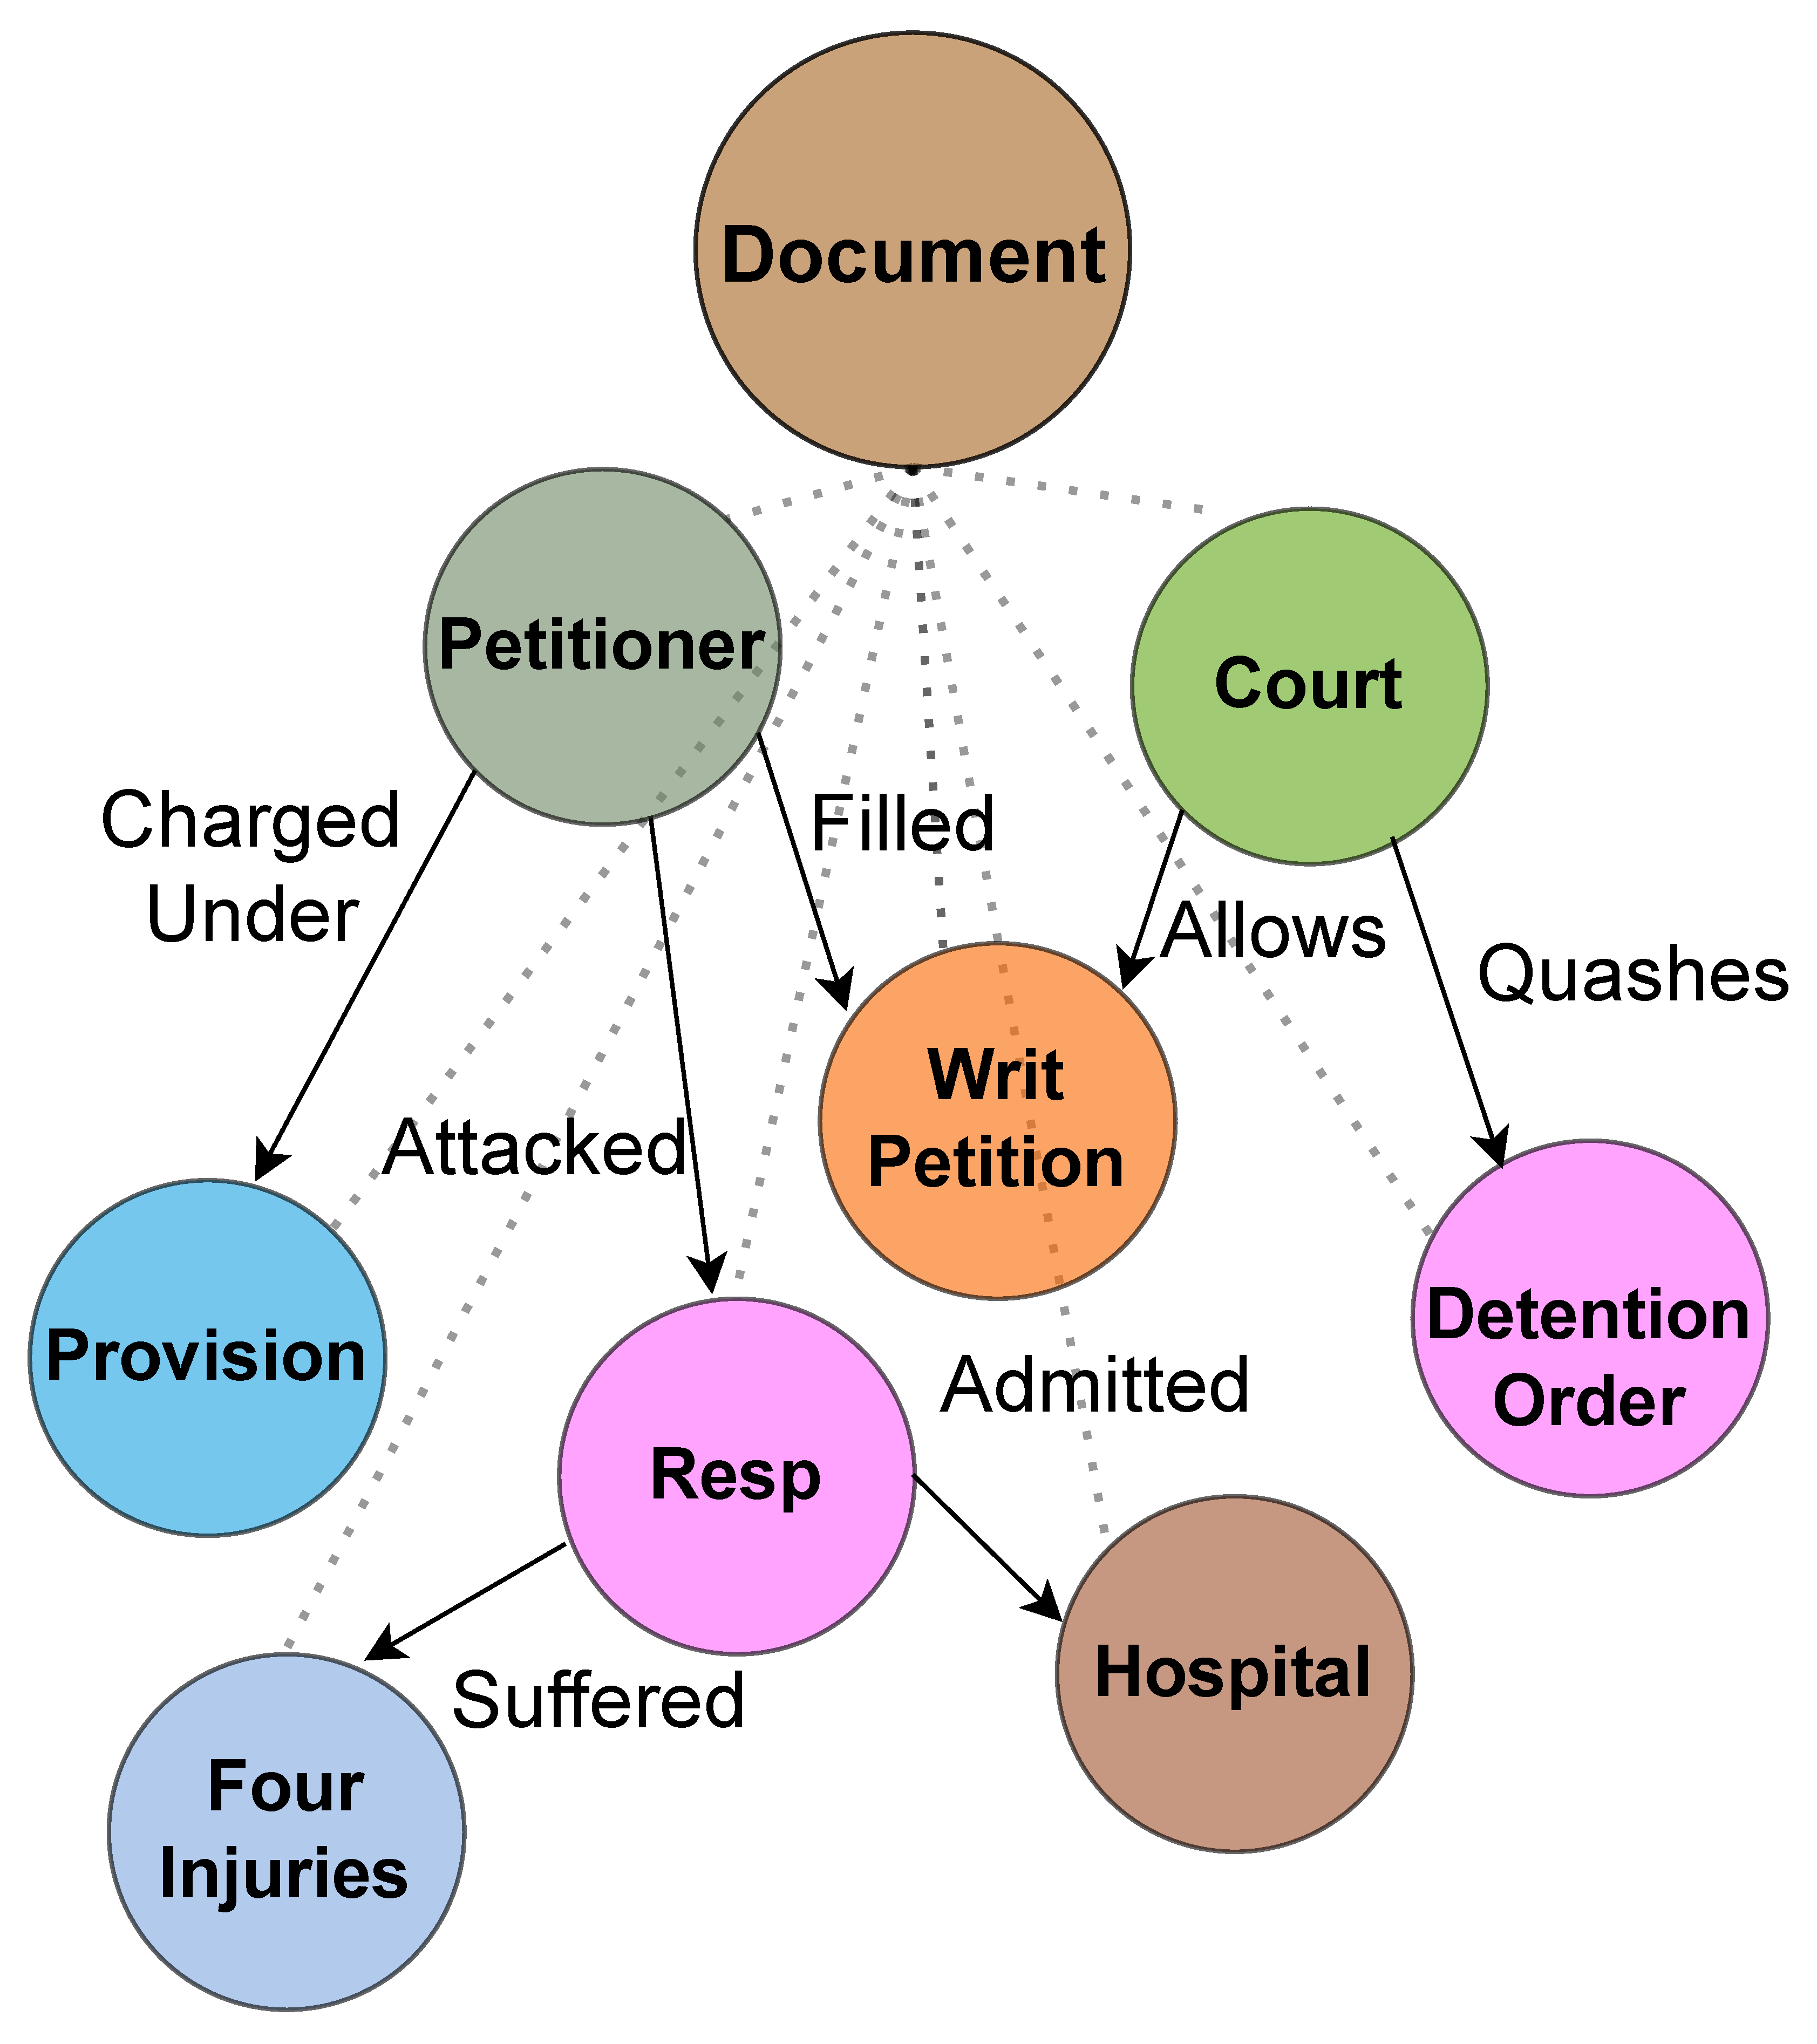
\includegraphics[scale=0.12,height=7cm]{./images/EventGNN.pdf}
    \vspace{-2mm}
    \caption{Part of the graph of a case document based on LLM-generated events (input for Event-GNN)}
    \label{fig:eventgnn}
    \vspace{-6mm}
\end{figure}

\noindent \textbf{2) SpaCy Events + BM25:} Prior works have demonstrated that both the queries and precedent candidates tend to be long and noisy, with only small portions of text leading to a strong match. \citet{joshi2023ucreat} used SpaCy (\url{www.spacy.io}) to extract events (subject, action, object triplets) and filtered out only the sentences containing matching events from both queries and precedents, leading to a better match. % via BM25. %We performed the same experiment.

\noindent\textbf{3) LLM Events + BM25:} We observed that SpaCy tends to over-generate events and is noisy. To address this, we employed an LLM (\texttt{gemma-7b-it}: \url{https://huggingface.co/google/gemma-7b-it}) to extract important events (prompt in Table~\ref{tab:event-llm-prompt}, App.~\ref{app:prompts}). We passed definitions from the SALI ontology (Standards Advancement for the Legal Industry: \url{https://www.sali.org/}) to guide the LLM in event generation. 
% We observed that LLM events are fewer than SpaCy events, but the elements in the (subject, action, object) triplets are larger (entire phrases/clauses) than that of SpaCy (one/two words at maximum). These events were subsequently used to filter out sentences for BM-25 baseline.
We found LLM events were fewer than SpaCy events but had larger triplet elements (subjects, actions, objects as full phrases/clauses vs. one–two words). These events were then used to filter sentences for the BM25 baseline.
%We observed that SpaCy generated a lot of events from a single query/candidate, which may not be ideal for the retrieval tasks. To customize this behavior, we employed an LLM (\texttt{gemma-7b-it}) to extract important events. We passed definitions from the SALI (Standards Advancement for the Legal Industry) (\url{https://www.sali.org/}) ontology to guide the LLM in event generation. We observed that LLM events are fewer than SpaCy events, but the elements in the (subject, action, object) triplets are larger (entire phrases/clauses) than that of SpaCy (one/two words at maximum). These events were subsequently used to filter out sentences for BM-25 baseline. % After extracting these events, we filtered out the sentences containing them and applied BM25 for the retrieval.

%\subsection{Semantic Methods} \label{sec:method/semantic}
%\vspace{2mm}
\vspace{1mm}
\noindent\underline{\textbf{Semantic Methods:}}
Semantic methods use deep-learning models trained on the train set. For fine-tuning, we explored two settings: (i)~training separate models for each task, and (ii)~a multi-task setup performing LSR and PCR simultaneously.

\noindent \textbf{1) SAILER:} \citet{li2023sailer} pre-trained a BERT-based model on legal documents to generate case reasoning and judgment from facts, then fine-tuned it for case retrieval on COLIEE 2021~\citep{rabelo2022coliee21}. We used this model for inference, with and without additional fine-tuning on our train set.


\noindent \textbf{2) Event-GNN:}
% Inspired by \citet{li2023findkg} we used GPT-4 (\texttt{gpt-4-turbo}: \url{https://platform.openai.com/docs/models/gpt-4-turbo})
% for creating event triplets for a small number ($\sim 400$) of documents from the train set and these triplets were subsequently used to fine-tune Gemma (\texttt{gemma-7b-it}) for generating triplets for the entire corpus. The triplets are used to create a graph with each subject and object being the nodes, and edges labeled with the action connecting the nodes (see App. Fig. \ref{fig:eventgnn}). 
% To reduce sparsity, we also introduced a global node to represent the whole document and connected each such global node with the global node of the cited case. All texts (corresponding to nodes (entity) and edges (relationships)) are encoded using SentenceBERT~\citep{reimers2019sentencebert}. We then employed a 2-layer Graph Attention Network~\citep{tang2024casegnn++} and perform dot product over the global nodes to capture document-level similarity between a query and candidate.
Inspired by \citet{li2023findkg}, we used GPT-4 (\texttt{gpt-4-turbo}: \url{https://platform.openai.com/docs/models/gpt-4-turbo}) to create event triplets for $\sim$400 training documents, then fine-tuned Gemma (\texttt{gemma-7b-it}) to generate triplets for the full corpus. Each triplet forms a graph where subjects/objects are nodes and actions label the edges (see Fig.~\ref{fig:eventgnn}). To reduce sparsity, a global node (connected to every subject/object node) represents each document and is linked to the global node of the cases it cites. Node (entity) and edge (relation) texts are encoded with SentenceBERT~\citep{reimers2019sentencebert}, and a 2-layer Graph Attention Network~\citep{tang2024casegnn++} computes document-level similarity via dot product over global nodes.


\noindent \textbf{3) Para-GNN:} 
% Different paragraphs in court case documents can usually be categorized into functional parts / rhetorical roles (from a legal perspective), such as Facts of the case, Arguments by lawyers, Ruling by the judge, etc.~\citep{malik-rr-2021}. The corpus source website IndianKanoon provides the rhetorical role for each paragraph, which can be used directly. Thus, we construct a setup where for each query/candidate, we have a global node representing the entire document and nodes for each paragraphs, connected to the global node with the edge labeled with the rhetorical role. The texts are converted to embeddings using SentenceBERT, and then a two-layer Graph Attention Network is employed on top. Dot product is calculated over the global nodes only. For statutes, each different subsection is taken as individual paragraphs, and the rhetorical role of each such paragraph is set to `None'.
Court case documents can be divided into segments such as Facts, Arguments, and Rulings~\citep{malik-rr-2021}, each performing a different rhetorical role from a legal perspective. IndianKanoon provides these labels per paragraph, which we use directly. For each query/candidate, we build a graph with a representative global node (whole document) and paragraph nodes linked to it via their rhetorical role. Texts are embedded with SentenceBERT, and a two-layer Graph Attention Network is applied, with dot product computed over global nodes. For statutes, each subsection is treated as a paragraph with role set to `None'.



%\subsection{Summary-based methods} \label{sec:method/summary}

\vspace{1mm}
%\vspace{2mm}
\noindent\underline{\textbf{Summary-based methods:}} 
% Using full case documents as both queries and precedents not only leads to large computation overload, but also introduces additional challenges for semantic models~\citep{tang2024caselink,tang2024casegnn++,qin2024ljpretrieval,yue2024eventcourtview}. 
% Full cases contain a lot of details that act as noise for statute and precedent retrieval. 
% Additionally, different portions of input text provide the contextual information needed for statute retrieval as compared to precedent retrieval. 
% Thus, we conducted summarization experiments to both reduce the noise and focus on the relevant contextual information. We used \texttt{GPT-4o-mini} (prompts in App. \ref{sec:expt/implementation/summ}) to summarize documents based on the two different retrieval needs. Note that we do not attempt to summarize the statute-texts, since statute-texts are usually short and well structured (as compared to case documents). On the precedent-side, we asked the LLM to focus on the legal rulings and findings of the case, which usually form the core reasons for future cases to cite these. 
% On the query-side, through  experimentation on the validation data, we found that it is difficult to generate one single coherent summary containing contextual information for both statute and precedent citations. This is because different portions of the query text provide the contextual information needed for LSR as compared to PCR.  Thus, for each query, we create two summaries, one focusing on LSR and the other focusing on PCR. For LSR-focused summaries, we asked the LLM to focus on the facts and legal issues of the case.
% For PCR-focused summaries, we asked the model to focus on the legal issues and arguments by lawyers, as well as findings of lower court. % (if any). 
% For joint retrieval, we concatenated the statute-retrieval and precedent-retrieval summaries to create a larger summary.
%The exact prompts used for summarization are in Appendix~\ref{sec:expt/implementation/summ}. 
Using full case documents as both queries and precedents causes computational overhead and poses challenges for semantic models~\citep{tang2024caselink,tang2024casegnn++,qin2024ljpretrieval,yue2024eventcourtview}. Full texts contain substantial noise for statute and precedent retrieval, and different text segments provide context relevant to LSR vs.\ PCR. To address this, we used summarization as a pre-processing step, aimed at reducing noise and highlighting task-specific context. We used \texttt{GPT-4o-mini} (\url{https://platform.openai.com/docs/models/gpt-4o-mini}) (prompts in App.~\ref{app:prompts}) to generate summaries tailored to each retrieval need. Statute texts were not summarized, as they are typically short and structured. For precedents, the LLM was asked to focus on legal rulings and findings, which are central for citation. On the query side, validation experiments showed that a single summary could not capture context for both LSR and PCR, since they rely on different parts of the text. Hence, for each query, we created two summaries: LSR-focused (tied to facts and legal issues of the query) and PCR-focused (tied to legal issues, lawyer arguments, and lower-court findings of the query). 
For joint fine-tuning, we concatenated the LSR and PCR-focused summaries to create a larger summary.
These prompt design decisions were formulated in close consultation with legal experts.

\begin{figure}[t]
    \centering
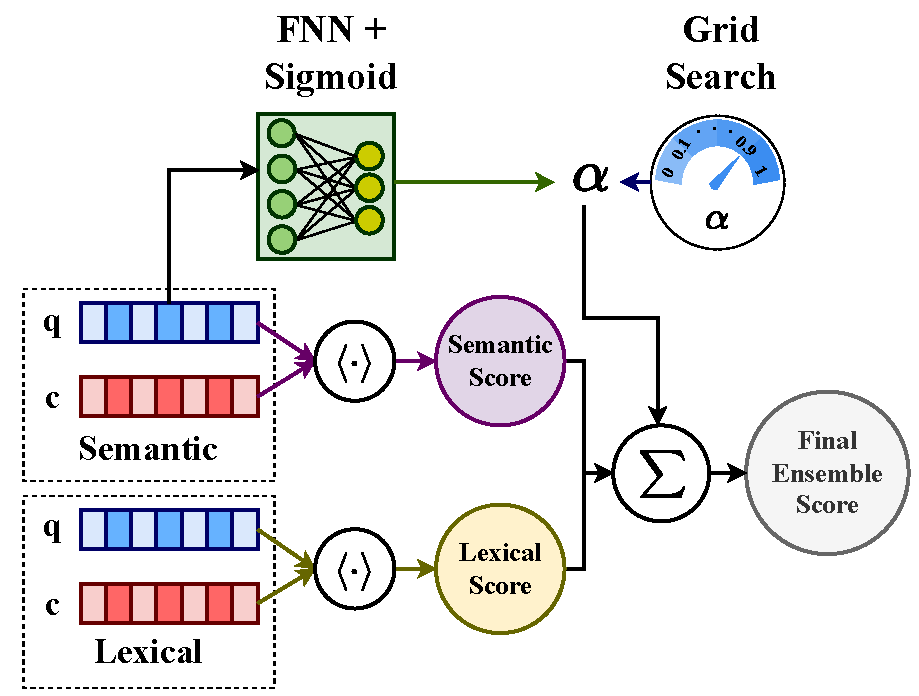
\includegraphics[width=0.45\textwidth]{./images/EnsembleGNN.pdf}
    \vspace{-2mm}
    \caption{Ensemble of lexical and semantic models. $\alpha$ can be tuned either via grid-search or dynamically learned via FFN.}
    \label{fig:ensemble}
    \vspace{-5mm}
\end{figure}


%\subsection{Paragraph-level retrieval methods}
%\vspace{2mm}
\vspace{1mm}
\noindent\underline{\textbf{Paragraph-level methods:}} %Since both the query and candidate documents are large, they can be split into natural paragraphs. 
%Since, original query and candidate documents are organized in the form of paragraphs. 
% We apply unsupervised methods directly at paragraph level for a query-candidate pair, and then aggregate the paragraph-level scores into a single document level score. Specifically, for a query $q$ having $n_q$ paragraphs and a candidate $c$ having $m_c$ paragraphs, we obtain a paragraph level $n_q \times m_c$ score matrix $M$. Then, we use two different aggregation measures:
% (i)~\textit{Max-All:} $\textrm{max}(M)$, and
% (ii)~\textit{Max-Sum:} $\sum_{i=1}^{n} \textrm{max}(M_i)$.
% We obtain the paragraph-level scores through BM25 2-gram and SAILER. We did not experiment with higher order n-grams since it was computationally prohibitive.
% Also, we could not fine-tune at the paragraph-level setup since we do not have the gold-standard information at the paragraph level.
We apply unsupervised methods at the paragraph level for each query–candidate pair, and then aggregate scores into a document-level score. For a query $q$ with $n_q$ paragraphs and candidate $c$ with $m_c$ paragraphs, we compute an $n_q \times m_c$ score matrix $M$. We use two aggregation measures: (i)~\textit{Max-All:} $\max(M)$, and (ii)~\textit{Max-Sum:} $\sum_{i=1}^{n_q} \max(M_i)$. We obtain Paragraph-level scores via BM25 2-gram and SAILER; higher-order n-grams were not attempted due to computational cost. Fine-tuning was also infeasible, as we do not have the ground-truth information at the paragraph level.


\begin{figure*}[t]
    \centering
    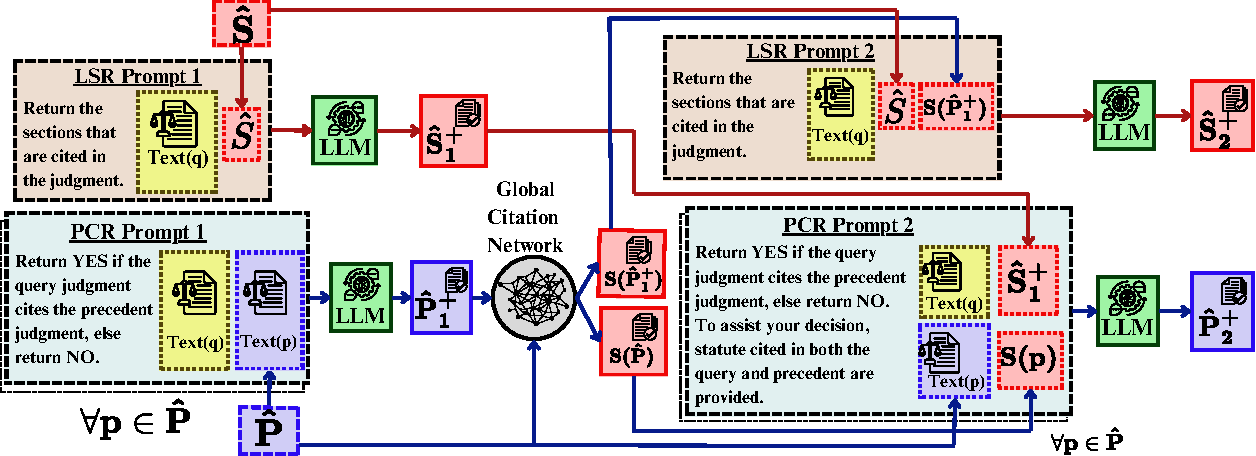
\includegraphics[scale=0.7]{./images/LLM_Reranking.pdf}
    %\includegraphics[width=\linewidth,height=5cm]{./images/EnsembleGNN.png}
    \vspace{-2mm}
    \caption{Proposed two-stage LLM prompting approach}
    \label{fig:llm-two-stages}
    \vspace{-3mm}
\end{figure*}

% \begin{figure}
%     \centering
%     \includegraphics[scale=0.15]{./images/demo_image.png}
%     %\includegraphics[width=\linewidth,height=5cm]{./images/EnsembleGNN.png}
%     \caption{Pipeline of the Ensemble-based approaches. QS and CS represent query and candidate semantic embeddings, while QL and CL represent the query and candidate lexical embeddings.}
%     \label{fig:ensemble}
%     \vspace{-5mm}
% \end{figure}
% \subsection{Ensemble of Lexical \& Semantic Methods} \label{sec:method/ensemble}
%\vspace{2mm}

\vspace{1mm}
\noindent\underline{\textbf{Ensemble of Lexical and Semantic Methods:}}
Combining lexical and semantic features can improve retrieval tasks~\citep{bruch2023fusionhybrid,sumathy2016hybridknowledge,mandikal2024sparsedensehybrid}. In the simplest form, we combine prediction scores for a query–candidate pair $(q,c)$ from lexical and semantic methods, where $c \in \mathcal S$ for LSR, or $c \in \mathcal P$ for PCR (see Fig.~\ref{fig:ensemble}). Formally, 
\vspace{-2mm}
\begin{align*}
\mathcal E(q,c) &= \alpha \times \textrm{Z-Norm}(\Sigma(q,c)) \\
   &\quad + (1 - \alpha) \times \textrm{Z-Norm}(\Lambda(q,c))
\end{align*}

\vspace{-2mm}
\noindent where $\mathcal E$ is the ensemble, $\Sigma$ the semantic method, $\Lambda$ the lexical method, and $\alpha$ a hyperparameter. As model scores vary in range, we apply Z-score normalization across all candidates per query. We use BM25 5-gram as the lexical method, and Event-GNN or Para-GNN as the semantic method.
We use the following two \textit{strategies to decide the optimal value of $\alpha$}:


\noindent\textbf{(1) Grid Search:} We vary the values of $\alpha = \{0, 0.1, \ldots, 0.9, 1\}$ for each task to determine the optimal value over the validation set. %This is done independently for statutes and precedents, and the optimal $\alpha$ value is used over the test set.

\noindent\textbf{(2) Dynamic $\mathbf{\alpha}$:} 
% In this approach, we try to learn the optimal $\alpha$ for each query by employing a feed-forward network (FFN) with sigmoid activation over the query embedding obtained from the semantic method. In the joint tuning setup, we used two separate FFNs for statute and precedent respectively. Apart from tuning independently and in multi-task learning setup, we tried a sequential approach as well, based on transfer learning. For instance, we took the statute model that was tuned independently, and used that to initialize the model for precedent tuning, and vice versa. This gave us models (obtained separately) for each task that were first trained on the other task to exploit the prospect of transfer learning properties between the two tasks.  We conduct in-depth analysis regarding the optimal $\alpha$ value for the different ensemble methods (see App.~\ref{app:gridsearch}).
In this approach, we learn the optimal $\alpha$ per query using a feed-forward network (FFN) with sigmoid activation over the query embedding from the semantic method. In joint tuning, separate FFNs are used for LSR and PCR. Beyond independent and multi-task setups, we also tested a sequential transfer-learning strategy: e.g., initializing the precedent model with the independently tuned statute model, and vice versa. This yielded task-specific models pre-trained on the other task, leveraging cross-task transfer. For further analyses of optimal $\alpha$ values, see App.~\ref{app:optimal-alpha}.

\vspace{1mm}
\noindent\underline{\textbf{Using LLMs for re-ranking:}} 
% Recently, LLMs have shown promising results for retrieval tasks.
% However, since the number of candidates in our setting is large and the texts of queries (and precedents in case of PCR) are very long, it makes it challenging to use LLM as a first-stage retriever. However, LLMs can be used as second-stage re-rankers, by re-ranking a limited number of candidates (say top $k$ candidates as given by any first stage retrieval model). Given the top-$k$ ranked list of candidates ($\hat{C}_k(q) = [c_{q_1}, c_{q_2}, \ldots, c_{q_k}]$) for a given query $q$ by a first stage retriever model $\mathcal M$, we ask the LLM $\mathcal G$ to give a binary relevance score $\mathcal G(q, c_{q_i}) \in \{0,1\}$ for each candidate in the top-$k$. All the subsequent notations are defined from the perspective of a single query $q$ and single chosen $k$ value, thus, for brevity, let us represent $\hat{C}_k(q)$ as $\hat C$.
% We then partition the top-$k$ ranked list as $\hat{C}^+ = \{c_{q_i} \mid \mathcal G(q, c_{q_i}) = 1\}$, and $\hat{C}^- = \{c_{q_i} \mid \mathcal G(q, c_{q_i}) = 0\}$. It is ensured that the original ordering (as per $\hat{C}$) is maintained between the candidates in both $\hat{C}^+$ and $\hat{C}^-$. Thereon, the re-ranked list becomes $\tilde{C}_k(q)$ or $\tilde{C} = \{\hat{C}^+, \hat{C}^-\}$. This ensures that the relevent candidates predicted by the LLM are ranked above those predicted as not relevant. We use a two-stage re-ranking pipeline for both tasks (Fig. ~\ref{fig:llm-two-stages}). % and described in detail below.
Recently, LLMs have shown strong results for retrieval. However, due to the large candidate space and the long texts of queries (and precedents in PCR), they are impractical as first-stage retrievers. Thus, we employ LLMs as second-stage re-rankers. A first-stage retriever $\mathcal M$ returns the top-$k$ list for query $q$:
\vspace{-2mm}
\[\hat{C}_k(q) = [c_{q_1}, c_{q_2}, \ldots, c_{q_k}].\]

\vspace{-2mm}
\noindent The LLM $\mathcal G$ assigns a binary relevance score $\mathcal G(q,c_{q_i}) \in \{0,1\}$ for each candidate. For brevity, let $\hat C := \hat{C}_k(q)$. We then partition $\hat C$ as
\vspace{-2mm}
\begin{align*}
\hat C^+ &= \{c_{q_i} \mid \mathcal G(q,c_{q_i})=1\}, \\
\hat C^- &= \{c_{q_i} \mid \mathcal G(q,c_{q_i})=0\},
\end{align*}

\vspace{-2mm}
\noindent while preserving the original ordering from $\hat C$ within both subsets. By construction,  $|\hat C^+| + |\hat C^-| = k$.
The final re-ranked list is
\vspace{-2mm}
\[\tilde C_k(q) = [\hat C^+, \hat C^-].\]

\vspace{-2mm}
\noindent This ensures that all LLM-predicted relevant candidates precede the non-relevant ones.  We adopt a two-stage re-ranking approach for both tasks. Fig.~\ref{fig:llm-two-stages} shows the entire pipeline for this.

\vspace{1mm}
\noindent\textbf{First-stage prompting:} 
% We first perform an initial stage of re-ranking, where LSR and PCR are performed independently. For statutes, for a given query $q$, we pass the full query text along with the names of \textit{all} the top-$k$ statutes $\hat S$ in the same prompt, and ask the LLM to directly return the set of statutes it considers relevant $\hat{S}_1^+ = \textrm{LLM}(\textrm{Text}(q), \hat{S})$. This approach is conditioned on the fact the LLM already has a prior knowledge of all the statutes $s \in \mathcal S$, and thus it already knows the statute texts. 
% For precedents, the LLM may not know the text of the precedent, and thus we pass the query and precedent text for each precedent $p$ in the top-$k$ precedents $\hat{P}$ in pair-wise fashion and ask it to predict if the pair is relevant. Thus, $\mathcal G_1(q, p) = \textrm{LLM}(\textrm{Text}(q), \textrm{Text}(p))$ and $\hat P_1^+ = \{p \mid p \in \hat P, \mathcal G_1(q,p)=1\}$.
We first perform an initial re-ranking stage where LSR and PCR are handled independently. For statutes, given a query $q$, we pass the full query text along with the names of all top-$k$ statutes $\hat S$ in a single prompt and ask the LLM to return the relevant subset: \vspace{-2mm} 
\[
\hat S_1^+ = \textrm{LLM}(\textrm{Text}(q), \hat S).
\]

\vspace{-2mm}
\noindent This assumes the LLM has prior knowledge of all statutes $s \in \mathcal S$, and therefore already knows their texts. 
For precedents, since the LLM may not know the precedent texts, we pass the query and each candidate precedent $p \in \hat P$ (top-$k$ precedents) in a pairwise fashion, asking if the pair is relevant:
\vspace{-2mm}
\begin{align*}
\mathcal G_1(q,p) &= \textrm{LLM}(\textrm{Text}(q), \textrm{Text}(p)), \\
\hat P_1^+ &= \{p \mid p \in \hat P, \ \mathcal G_1(q,p)=1\}.
\end{align*}

\vspace{-1mm}
\noindent\textbf{Second-stage prompting:} 
% From the first stage prompting, we obtained the initial predictions $\hat S_1^+$ and $\hat P_1^+$ for LSR and PCR respectively.
% In the second stage, we wish to utilize the relationship between LSR and PCR in a sequential fashion, using the outputs of one task to try improve the other. For performing LSR, we first take the positive precedents of PCR re-ranking (first stage), $\hat{P}_1^+$, and collect all ground-truth statutes cited by these precedents $S(\hat{P}_1^+) = \cup_{p \in \hat{P}_1^+} S(p)$, where the $S(.)$ function represents the mapping from any query, or precedent, to its ground-truth statutes. This ground-truth information is known to us during test time since precedents are not masked. These additional statutes are passed to the prompt along with the top-$k$ statute ranked list $\hat S$, to obtain the second-stage re-ranked predictions: $\hat{S}_2^+ = \textrm{LLM}(\textrm{Text}(q), \hat{S} \cup S(\hat{P}_1^+))$. We effectively increase the re-ranking range of the LLM in an informed way, utilizing the connection between precedents and the ground-truth cited statutes. % cited by them.
From the first-stage prompting, we obtain the initial predictions $\hat S_1^+$ and $\hat P_1^+$ for LSR and PCR respectively.  
In the second stage, we leverage the relationship between LSR and PCR sequentially, using the output of one task to improve the other. For LSR, we take the positive precedents from first-stage PCR re-ranking ($\hat P_1^+$) and collect all ground-truth statutes cited by these precedents:
\vspace{-2mm}
\[
S(\hat P_1^+) = \bigcup_{p \in \hat P_1^+} S(p),
\]

\vspace{-2mm}
\noindent where $S(\cdot)$ denotes the mapping from any query or precedent to its ground-truth statutes. This ground-truth is available at test time since precedents are not masked.  
These additional statutes are then passed to the prompt, together with the top-$k$ statute list $\hat S$, to obtain the second-stage predictions:
\vspace{-2mm}
\[
\hat S_2^+ = \textrm{LLM}(\textrm{Text}(q), \hat S \cup S(\hat P_1^+)).
\]

\vspace{-1mm}
\noindent Thus, we expand the re-ranking range of the LLM in an informed manner, exploiting the connection between precedents and their cited statutes.


% \noindent For second-stage precedent re-ranking, we first consider the positive statutes $\hat{S}_1^+$ for the query $q$ as per LCR first-stage re-ranking, and the ground truth statutes $S(p)$ for a precedent $p$, and pass these names to the prompt along with the texts of $q$ and $p$ to get the second-stage PCR mapping $\mathcal G_2(q,p) = \textrm{LLM}(\textrm{Text}(q), \hat{S}_1^+, \textrm{Text}(p), S(p)), \forall p \in \hat{P}$, and thus $\hat P_2^+ = \{p \mid p \in \hat P, \mathcal G_2(q,p)=1\}$. The idea here is that the LLM should be able to exploit the statute information to better judge relevance between $q$ and $p$ for PCR. %We use the predicted statutes for the query and the gold-standard statutes for the precedent.
\noindent For second-stage precedent re-ranking, we use the positive statutes $\hat S_1^+$ for query $q$ (from first-stage LSR) together with the ground-truth statutes $S(p)$ for each precedent $p$. These statute names are passed to the prompt along with the texts of $q$ and $p$, yielding the second-stage PCR mapping:
\vspace{-2mm}
\begin{align*}
\mathcal G_2(q,p) &= \textrm{LLM}\big(\textrm{Text}(q), \hat S_1^+, \nonumber \\
&\quad\ \ \textrm{Text}(p), S(p)\big), \quad \forall p \in \hat P, \\
\hat P_2^+ &= \{p \mid p \in \hat P, \mathcal G_2(q,p)=1\}.
\end{align*}

\vspace{-2mm}
\noindent The intuition is that by conditioning on statute information, the LLM can better assess the relevance of precedents to the query in PCR.
All prompts are shown in brief in Fig.~\ref{fig:llm-two-stages} (full prompts in App.~\ref{app:prompts}).

% \vspace{2mm}
% \noindent\underline{\textbf{Setup and Hyperparameters:}}
% For BM25-based experiments, we used different n-grams ($n=2,3,4,5$). In case of the fine-tuning approaches, we use a contrastive learning setup, with BM25 hard negatives and in-batch negative sampling. We used  AdamW~\citep{loshchilov2017adamw} optimizer and a linear scheduler. \paul{For re-ranking, we used GPT-4.1 and chose top $k=20$ for statutes and $k=10$ for precedents.} For more details see App. \ref{app:implementation}. %Exact details of the setup and hyper-parameter settings are provided in Appendix~\ref{app:implementation}.
% \vspace{2mm}
% \noindent\textbf{Grid Search:} We vary the values of $\alpha = \{0, 0.1, \ldots, 0.9, 1\}$ to determine the optimal value over the validation set. This is done independently for statutes and precedents, and the optimal $\alpha$ value is used over the test set.

% \vspace{2mm}
% \paul{\noindent\textbf{Dynamic $\mathbf{\alpha}$:} In this approach, we try to learn the optimal $\alpha$ for each query by employing a feed-forward network (FFN) with sigmoid activation over the query embedding obtained from the semantic method. In the joint tuning setup, we used two separate FFNs for statute and precedent respectively. Apart from tuning independently and in multi-task learning setup, we tried a pipeline approach as well. We took the statute model tuned independently, and used that to initialize the model for precedent tuning, and vice versa for statute tuning. This gave us models (obtained separately) for each task that were first trained on the other task to exploit the prospect of transfer-learning properties between the two tasks.} 

%\subsection{Usage of LLMs in retrieval methods}
% \vspace{2mm}
% \noindent\underline{\textbf{Usage of LLMs in retrieval methods:}} %Generative LLMs have transformed the NLP space lately, producing superior performance on many tasks. However, 
% It is difficult to use LLMs directly for retrieval purposes, since the model must be fed the query text as well as \textit{all the candidate texts} in the same prompt window. 
% This is not straight-forward in the legal domain since we have a large number of candidates, and the texts are quite lengthy. We instead use LLMs to restructure the input for downstream retrieval models, by creating events  or summaries. 
%We instead use LLMs to restructure the input for downstream retrieval models, by creating events (in Event-GNN)
%(Section~\ref{sec:method/semantic}) 
%or summaries, as described above. %(Section~\ref{sec:method/summary}).

% \noindent\underline{\textbf{Using LLMs for re-ranking:}} 
% \paul{It is difficult to use LLMs as first stage retrievers, since the number of candidates is large and the texts of queries (and precedents in case of PCR) are very long. However, LLMs can be used as second-stage re-rankers, by re-ranking a limited number of candidates (say top $k$ candidates as given by any first stage retrieval model) for each query. Given the top-$k$ ranked list of candidates for a given query $q$ by a first stage retriever model $\mathcal M$, $\hat{C}_k(q) = [c_{q_1}, c_{q_2}, \ldots, c_{q_k}]$, we ask the LLM $\mathcal G$ to give a binary relevance score $\mathcal G(q, c_{q_i}) \in \{0,1\}$ for each candidate in the top-$k$.}
% \paul{\textit{All further notations are defined from the perspective of a single query $q$ and single chosen $k$ value, thus, for brevity, let us represent $\hat{C}_k(q)$} as $\hat C$.}
% \paul{We then partition the top-$k$ ranked list as $\hat{C}^+ = \{c_{q_i} \mid \mathcal G(q, c_{q_i}) = 1\}$, and $\hat{C}^- = \{c_{q_i} \mid \mathcal G(q, c_{q_i}) = 0\}$. It is ensured that the original ordering (as per $\hat{C}$) is maintained between the candidates in both $\hat{C}^+$ and $\hat{C}^-$. Thereon, the re-ranked list becomes $\tilde{C}_k(q)$ or $\tilde{C} = \{\hat{C}^+, \hat{C}^-\}$. This ensures that the candidates predicted relevant by the LLM are ranked ahead of those predicted as not relevant.
% We use a two-stage re-ranking pipeline for both tasks, which is shown in Figure~\ref{fig:llm-two-stages}, and described in detail below.}

% \noindent\textbf{First-stage prompting:} \paul{We first perform an initial stage of re-ranking, where LSR and PCR are performed independently. For statutes, for a given query $q$, we pass the full query text along with the names of \textit{all} the top-$k$ statutes $\hat S$ in the same prompt, and ask the LLM to directly return the set of statutes it considers relevant $\hat{S}_1^+ = \textrm{LLM}(\textrm{Text}(q), \hat{S})$. This approach is conditioned on the fact the LLM already has a prior knowledge of all the statutes $s \in \mathcal S$, and thus it already knows the statute texts. 
% For precedents, the LLM may not know the text of the precedent, and thus we pass the query and precedent text for each precedent $p$ in the top-$k$ precedents $\hat{P}$ in pair-wise fashion and ask it to predict if the pair is relevant. Thus, $\mathcal G_1(q, p) = \textrm{LLM}(\textrm{Text}(q), \textrm{Text}(p))$ and $\hat P_1^+ = \{p \mid p \in \hat P, \mathcal G_1(q,p)=1\}$.}


% \noindent\textbf{Second-stage prompting:} 
% \paul{From the first stage prompting, we have obtained the initial predictions $\hat S_1^+$ and $\hat P_1^+$ for LSR and PCR respectively.}
% \paul{In the second stage, we wish to utilize the relationship between LSR and PCR in a pipeline fashion, using the outputs of one task to try improve the other. For performing LSR, we first take the positive precedents of PCR re-ranking (first stage), $\hat{P}_1^+$, and collect all ground-truth statutes cited by these precedents $S(\hat{P}_1^+) = \cup_{p \in \hat{P}_1^+} S(p)$, where the $S(.)$ function represents the mapping from any query, or precedent, to its ground-truth statutes. This ground-truth information is known to us during test time since precedents are not masked. Thereon, we simply pass these additional statutes to the prompt along with the top-$k$ statute ranked list $\hat S$, to obtain the second-stage re-ranked predictions: $\hat{S}_2^+ = \textrm{LLM}(\textrm{Text}(q), \hat{S} \cup S(\hat{P}_1^+))$. We effectively increase the re-ranking range of the LLM in an informed way, utilizing the connection between precedents and the ground-truth statutes cited by them.}

% \paul{For second-stage precedent re-ranking, we first consider the positive statutes $\hat{S}_1^+$ for the query $q$ as per LCR first-stage re-ranking, and the ground truth statutes $S(p)$ for a precedent $p$, and pass these names to the prompt along with the texts of $q$ and $p$ to get the second-stage PCR mapping $\mathcal G_2(q,p) = \textrm{LLM}(\textrm{Text}(q), \hat{S}_1^+, \textrm{Text}(p), S(p)), \forall p \in \hat{P}$, and thus $\hat P_2^+ = \{p \mid p \in \hat P, \mathcal G_2(q,p)=1\}$. The idea here is that the LLM should be able to exploit the statute information to better judge relevance between $q$ and $p$ for PCR. We use the predicted statutes for the query and the gold-standard statutes for the precedent.}

% \vspace{2mm}
% \noindent\underline{\textbf{Setup and Hyperparameters:}}
% For BM25-based experiments, we used different n-grams ($n=2,3,4,5$). In case of the fine-tuning approaches, we use a contrastive learning setup, with BM25 hard negatives and in-batch negative sampling. We used  AdamW~\citep{loshchilov2017adamw} optimizer and a linear scheduler. \paul{For re-ranking, we used GPT-4.1 and chose top $k=20$ for statutes and $k=10$ for precedents.} For more details see App. \ref{app:implementation}. %Exact details of the setup and hyper-parameter settings are provided in Appendix~\ref{app:implementation}.



% \begin{table*}
%     \centering
%     \small
%     \begin{tabular}{p{0.18\textwidth}p{0.30\textwidth}cccccc}
%          \hline
%          \textbf{Ensemble Method} & \textbf{Setting} & \multicolumn{3}{c}{\textbf{Statutes}} & \multicolumn{3}{c}{\textbf{Precedents}} \\ 
%           & & \textbf{F1} & \textbf{MAP} & \textbf{MRR} & \textbf{F1} & \textbf{MAP} & \textbf{MRR} \\ \hline

%           Event-GNN + BM25 & Grid Search & \textbf{33.87} & \textbf{45.17} & \textbf{67.26} & 34.45 & 43.32 & 58.76 \\
%           & Dynamic $\alpha$, finetune separately & 30.29 & 40.97 & 61.51 & 35.60 & 45.86 & 60.89 \\
%           & Dynamic $\alpha$, finetune multi-task & 25.62 & 31.97 & 57.01 & 35.63 & 45.18 & 60.51 \\ \hline
%           Para-GNN + BM25 & 5-gram, Grid Search & 28.10 & 36.14 & 59.57 & \textbf{36.93} & \textbf{48.62} & \textbf{62.83} \\
%           & Dynamic $\alpha$, finetune separately & 27.05 & 35.20 & 59.67 & 36.91 & 48.53 & 62.61 \\
%           & Dynamic $\alpha$, finetune multi-task & 27.01 & 33.57 & 59.00 & 36.57 & 48.18 & 62.14 \\ \hline
%           Para-GNN (summaries) + BM25 & Grid Search & 36.17 & 48.64 & 70.49 & 36.35 & 48.27 & 61.76 \\ \hline
%     \end{tabular}
%     \caption{Results of ensemble methods for both LSR and PCR tasks. Best value for each metric in boldface. \paul{Ensemble summaries fine-tuning TBD}}
%     \label{tab:ensemble}
%     \vspace{-5mm}
% \end{table*}



% \begin{table*}
%     \centering
%     \small
%     \begin{tabular}{lcccccc}
%         \hline
%         \textbf{Method} & \multicolumn{3}{c}{\textbf{Statutes}} & \multicolumn{3}{c}{\textbf{Precedents}} \\
%         & Lexical & Semantic & Ensemble & Lexical & Semantic & Ensemble \\ \hline
%         Para-GNN (GridSearch) & 16.98 & 20.72 & 28.10 & 33.29 & 24.54 & 36.93 \\
%         Para-GNN (dynamic) &  16.98 & 20.72 & 27.05 & 33.29 & 24.54 & 36.91 \\ \hline
%         Event-GNN (GridSearch) & 16.98 & 28.67 & 33.87 & 33.29 & 12.08 & 34.45 \\ 
%         Event-GNN (dynamic) &   &  &  &  &  & \\ \hline
%     \end{tabular}
%     \caption{Performance (macro-F1@K in \%) of ensemble models compared with the default lexical and semantic approaches \sg{I find the format of this table very confusing. It seems the entire row is for the method stated on the left, but it is not so. Why can we not use the same format as in Table~\ref{tab:results}?}}
%     \label{tab:ensemble}
% \end{table*}






% \subsection{Ensemble of Lexical and Semantic Methods}

% We also experimented with an ensemble setup to combine the effect of lexical and semantic methods. In the simplest setup, we can combine the prediction (score) of assigned to a particular (query, candidate) pair by a lexical method with that given by semantic methods. Formally, $\textrm{Score}(Q,C) = \alpha \times \textrm{Semantic Norm Score}(Q,C) + (1 - \alpha) \times \textrm{Lexical Norm Score}(Q,C)$. We need the normalized scores since the default scores coming from the models can be of different scales; here we performed Z-score normalization across all candidates for each query. In the ensemble approaches, we used BM25 5-gram as the lexical method and Event-GNN or RR-GNN as the semantic method.

% \noindent\textbf{Grid Search for Best $\alpha$:} We vary the values of $\alpha = \{0, 0.1, 0.2, \ldots, 0.9, 1\}$, and determine the optimal setting.

% \noindent\textbf{Dynamic $\alpha$:} We tune a feed-forward network with sigmoid activation on top of the semantic embeddings to generate the $\alpha$ value dynamically according to each query. The semantic methods are fine-tuned along with the linear layer.





%\vspace{-2mm}
\section{Experiments, Results and Analysis} \label{sec:expt}
%\vspace{-2mm}
% \begin{figure*}[!thb]
% \centering
% \begin{subfigure}[t]{.35\textwidth}
%   \centering
%   \includegraphics[width=\linewidth]{./images/EventGNN.png}
%   \caption{Event-GNN}
%   \label{fig:ilsi-lfreq-ilb}
% \end{subfigure}%
% % \begin{subfigure}[t]{.24\textwidth}
% %   \centering
% %   \includegraphics[width=\linewidth]{./images/ParaGNN.png}
% %   \caption{Para-GNN}
% %   \label{fig:ilsi-lfreq-lf}
% % \end{subfigure}%
% \begin{subfigure}[t]{.60\textwidth}
%   \centering
%   \includegraphics[width=\linewidth]{./images/EnsembleGNN.png}
%   \caption{Ensemble}
%   \label{fig:echr-lfreq-ilb}
% \end{subfigure}%
% %\vspace{-4mm}
% \caption{Diagram of methods}
% %\vspace{-5mm}
% \label{fig:analysis-lfreq}
% \end{figure*}
%\subsection{Implementation Details} \label{sec:expt/implementation}
%\noindent\textbf
\begin{table*}[!thb]
    \centering
    \small
    \begin{tabular}{p{0.24\textwidth}p{0.22\textwidth}cccccc}
         \toprule
         \textbf{Method} & \textbf{Setting} & \multicolumn{3}{c}{\textbf{LSR}} & \multicolumn{3}{c}{\textbf{PCR}} \\
          & & \textbf{F1} & \textbf{MAP} & \textbf{MRR} & \textbf{F1} & \textbf{MAP} & \textbf{MRR} \\ \midrule 
        \multicolumn{8}{c}{\textbf{Lexical Methods}}\\ \midrule 
 
         \multirow{4}{0.24\textwidth}{Vanilla BM25 (full doc)} & 2-gram & 13.15& 14.54& 32.36& 24.89& 32.41& 47.21\\
          & 4-gram & 17.06& 19.13& 40.88& 30.54& 40.24& 54.65\\ 
          & 3-gram & 17.80& 19.39& 41.74& 32.21& 43.44& 57.52\\ 
          & 5-gram & 16.98& 17.88& 40.08& 33.29* & 43.98* & 58.55*\\ \midrule 

        \multirow{2}{0.24\textwidth}{Vanilla BM25 (para-wise)} & 2-gram, Max-All & 18.59& 21.82& 44.32& 27.87& 38.15& 52.32\\
        & 2-gram, Max-Sum & 14.66& 16.67& 35.84& 26.23& 35.26& 49.41\\ \midrule 
        

        
         \multirow{4}{0.24\textwidth}{Spacy events + BM25 (full doc)} & 2-gram & 12.65 & 14.48 & 32.08 & 24.91 & 33.02  & 48.22 \\
         & 3-gram & 10.67 & 11.93 & 28.12 & 28.31 & 37.22 & 52.70 \\
         & 4-gram & 10.18 & 10.47 & 26.40 & 28.28 & 35.30 & 50.98 \\
         & 5-gram & 9.78 & 9.52 & 25.28 & 26.99 & 33.71 & 50.22 \\ \midrule 
         
         \multirow{4}{0.24\textwidth}{LLM events + BM25 (full doc)} & 2-gram & 13.08& 14.47& 32.49& 24.55& 31.78& 46.10\\
         & 3-gram & 16.84& 18.76& 40.60& 29.47& 38.59& 52.97\\
         & 4-gram & 17.45& 18.92& 41.34& 32.61& 42.99& 57.39\\
         & 5-gram & 16.41& 17.35& 39.33& 33.29& 43.43& 58.14\\ \midrule 
         


         \multicolumn{8}{c}{\textbf{Semantic Methods}}\\ \midrule 

         
         \multirow{3}{0.24\textwidth}{SAILER (full doc)} & inference  & 7.15& 9.31& 19.40& 9.94& 13.90&20.49\\
         & fine-tune separately  & 21.69 & 28.62& 45.73&  12.64& 17.93&  25.85\\ 
         & fine-tune multi-task & 20.45& 25.36& 41.44& 11.88& 17.52& 24.85\\ \midrule 
         
         \multirow{2}{0.24\textwidth}{SAILER (para-wise)} & inference, Max-All & 13.11 & 14.70 & 31.49 & 19.37 & 25.71 & 38.84  \\
        & inference, Max-Sum & 5.42 & 6.57 & 16.06 & 11.16 & 16.42 & 24.67 \\ \midrule 
        \multirow{2}{0.24\textwidth}{SAILER (summaries)} & inference & 5.48& 7.66& 16.86& 10.21& 14.80& 22.82\\
        & fine-tune separately & 23.49& 31.42& 50.25& 15.00& 20.43& 27.72\\ \midrule 
        
         \multirow{2}{0.24\textwidth}{Event-GNN (full doc)} & fine-tune separately & 28.67 & 38.69 & 58.39&  12.08& 15.91&  22.18\\ 
         & fine-tune multi-task & 18.43& 24.11& 43.23& 11.74& 15.59& 22.56\\ \midrule 
         \multirow{2}{0.24\textwidth}{Para-GNN (full doc)} & fine-tune separately & 20.72& 28.54& 46.06&  24.54  & 33.07& 45.01\\ 
         & fine-tune multi-task & 23.74& 29.79& 49.84&  24.67& 32.88& 44.17\\ \midrule 
         
        
         \multirow{2}{0.24\textwidth}{Para-GNN (summaries)} & fine-tune separately & 32.85* & 44.03* & 62.51&   22.60& 29.49& 39.22\\ 
         & fine-tune multi-task & 31.81& 43.17& 64.08* & 22.69& 29.25& 39.19\\ \midrule 
         
         \multicolumn{8}{c}{\textbf{Ensemble Methods}}\\ \midrule 
         \multirow{3}{0.24\textwidth}{Event-GNN + BM25} & Grid Search & 33.87 & 45.17 & 67.26 & 34.45 & 43.32 & 58.76 \\
         & Dyn. $\alpha$, fine-tune separately & 30.29 & 40.97 & 61.51 & 35.60 & 45.86 & 60.89 \\
         & Dyn. $\alpha$, fine-tune multi-task & 25.62 & 31.97 & 57.01 & 35.63 & 45.18 & 60.51 \\ \midrule 
          \multirow{3}{0.24\textwidth}{Para-GNN (full doc) + BM25} & Grid Search & 28.10 & 36.14 & 59.57 & 36.93 & 48.62 & 62.83 \\
          & Dyn. $\alpha$, fine-tune separately & 27.05 & 35.20 & 59.67 & 36.91 & 48.53 & 62.61 \\
          & Dyn. $\alpha$, fine-tune multi-task & 27.01 & 33.57 & 59.00 & 36.57 & 48.18 & 62.14 \\ \midrule 
          \multirow{4}{0.24\textwidth}{Para-GNN (summaries) + BM25} & Grid Search& 36.17 & 48.64 & 70.49 & 36.35 & 48.27 & 61.76 \\
          & Dyn. $\alpha$, fine-tune separately & 38.09&  50.31&  70.54& 37.46 &  48.28&  61.98\\
          & Dyn. $\alpha$, fine-tune multi-task & 35.91 &  46.95&  68.57& 37.82 &  49.54&  63.61\\
          & Dyn. $\alpha$, fine-tune transfer learning & \underline{39.44}&  \underline{52.13}&  \underline{73.77}& \underline{38.77}&  \underline{50.21}&  \underline{63.81}\\ \midrule 
          \multicolumn{8}{c}{\textbf{LLM Re-ranking}}\\ \midrule 
          \multirow{2}{0.24\textwidth}{GPT-4.1} & First-stage prompt & 45.29& 59.73& 81.02& 41.54& 52.80& 67.16\\
          & Second-stage prompt & \textbf{46.11}& \textbf{61.06}& \textbf{81.55}& \textbf{43.31}& \textbf{54.43}& \textbf{68.88}\\
          \bottomrule
         % \hline
    \end{tabular}
    \vspace{-2mm}
    \caption{Results (\%) of Statute retrieval and Precedent retrieval. Metrics are macro-F1@k, MAP and MRR. Best value for each metric in boldface. Best values before re-ranking underlined, and best values for individual methods (not ensemble methods) marked with asterisk(*). We also calculate statistical significance of results  (App.~\ref{app:sigtest}).}
    \label{tab:results}
    \vspace{-5mm}
\end{table*}
%\vspace{-2mm}
%\subsection{Results} \label{sec:expt/results}
%\vspace{-2mm}
% \old{The results of all methods are presented in Table~\ref{tab:results} in terms of standard evaluation metrics macro-F1@k, MAP and MRR (details in App. \ref{app:expt/datasets}). We observe a stark difference in the performance of different methods for statutes and precedents.  
% Methods based on BM25, which focus on lexical matches and hence can capture legal phrases or keywords, are very effective for precedent retrieval.
% Whereas, fine-tuned transformer models are able to perform better for statute retrieval than unsupervised lexical methods.
% %, where all the fine-tuning approaches significantly outperform the unsupervised approaches. 
% The language used in statute descriptions is more formal than that used in case documents, and thus direct keyword matching can be difficult. This could explain why supervised fine-tuning is performing the best. 
% %We also observe that tuning statutes and precedents jointly in a multi-task learning setup does not perform as well as the setup where they are tuned separately (more on this in Section~\ref{sec:expt/results/statprec}).
% Also, we observe that summarization leads to an improvement in performance only for statutes, but not precedents (compared to taking the full documents as input).}

\noindent The results of all experiments are presented in Table~\ref{tab:results} in terms of standard evaluation metrics macro-F1@$k$, MAP and MRR (details in App.~\ref{app:expt/datasets}, hyper-parameters in App.~\ref{app:implementation}). 

\vspace{1mm}
\noindent\underline{\textbf{Performance over LSR:}} 
% We observe that the lexical approaches perform rather poorly over LSR, possibly due to the abstract and technical language used for statutes. 
% While the para-wise variant of BM25 improves results, these are quite poor compared to the performance of semantic, fine-tuned methods. 
% Among these, utilizing the LLM retrieval-focussed summaries with the Para-GNN architecture proves the most effective (32.85\% F1), while summaries over full document input are helpful for other methods like SAILER as well. 
Lexical methods perform poorly on statute retrieval, likely due to the abstract and technical phrasing of statutes. Even the best lexical variant (BM25, para-wise Max-All) achieves only 18.59\% F1. In contrast, fine-tuned semantic models show large gains, with Para-GNN (summaries) reaching 32.85\% F1---a relative improvement of nearly 77\%. This highlights the need for deeper contextual modeling. Summaries also help other semantic models such as SAILER, though the gains are smaller. 

\vspace{1mm}
\noindent\underline{\textbf{Performance over PCR:}} 
% In the case of PCR, we observe the reverse trends as compared to LSR. The semantic, fine-tuning based methods underperform as compared to lexical methods like BM25. Among these, Para-GNN again performs the best, although there is a slight drop in performance on using summaries over full documents. We suspect that PCR depends on exact lexical matches over short contextual windows for both queries and precedents, and thus using summaries can lead to information loss. In a broader sense, the same factor, coupled with the fact that both queries and precedents are long documents makes the task non-conducive for semantic fine-tuning methods.
In contrast to LSR, lexical methods clearly dominate PCR. The best lexical model (BM25, 5-gram) achieves 33.29\% F1, whereas the strongest semantic model (Para-GNN, full doc, fine-tuned) reaches only 24.67\% F1, a relative drop of about 26\%. Moreover, summaries further reduce performance, suggesting that essential lexical cues are lost during compression. These results indicate that PCR depends heavily on exact lexical matches within short contextual windows, and the long, detailed nature of queries and precedents makes semantic fine-tuning less effective. 



\begin{figure*}
\begin{subfigure}[t]{.47\linewidth}
  \centering
  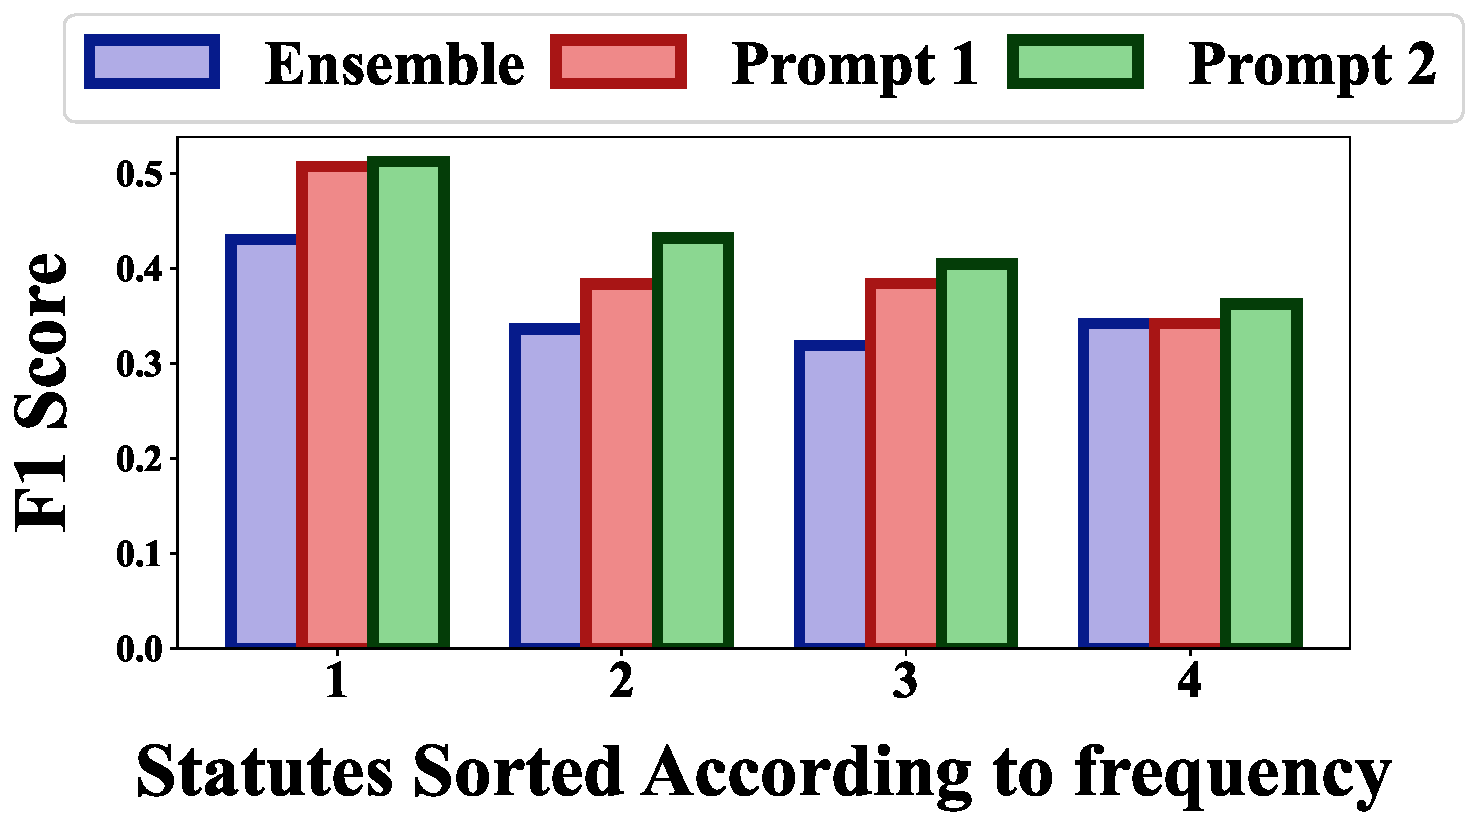
\includegraphics[width=\linewidth]{./images/llm-freq-lsr.pdf}
  \caption{LSR F1 vs. frequency}
  \label{fig:llm-freq-lsr}
\end{subfigure}%
\hfill
\begin{subfigure}[t]{.47\linewidth}
  \centering
  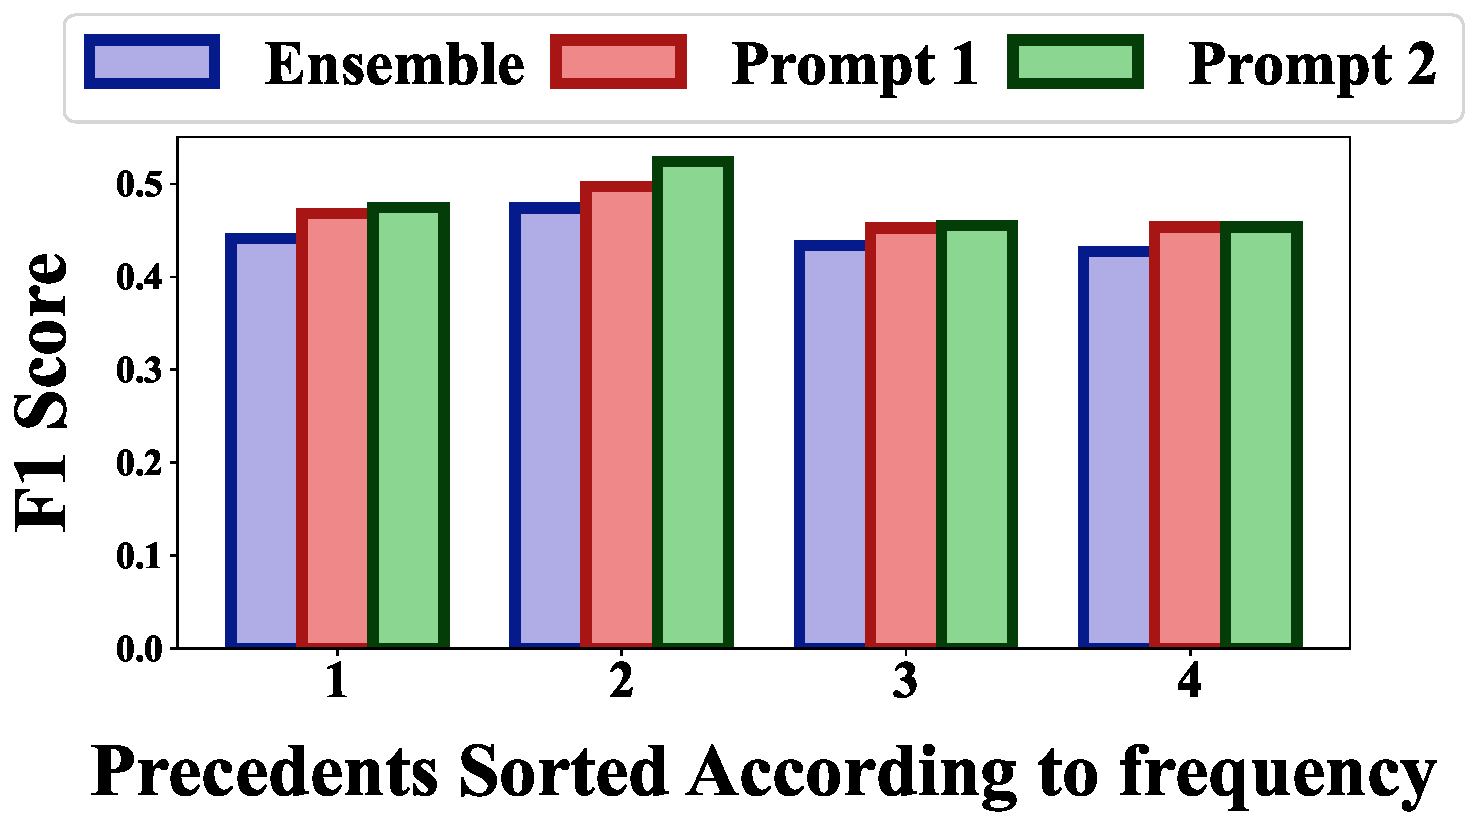
\includegraphics[width=\linewidth]{./images/llm-freq-pcr.pdf}
  \caption{PCR F1 vs. frequency}
  \label{fig:llm-freq-pcr}
\end{subfigure}%
\vspace{-2mm}
\caption{Performance in terms of F1(\%) compared to frequency of candidates. On the X-axis, the candidates are sorted from left to right according to frequency and divided into groups (most frequent group-1, most rare group-4).} 
\label{fig:llm-freq}
\vspace{-5mm}
\end{figure*}

\vspace{1mm}
\noindent\underline{\textbf{Results of Ensemble Models:}}
% The ensemble approaches achieve improvements for both statutes and precedents, compared to both the individual lexical and semantic methods. This is true for all three variants of the semantic method (Event-GNN, Para-GNN with full docs and summaries). Although the dynamic $\alpha$ method slightly underperforms compared to grid search for Event-GNN + BM25 and Para-GNN (full doc) + BM25, there are clear gains over grid search in the case of Para-GNN (summaries) + BM25 for both LSR (38.09\% vs. 36.17\% F1) and PCR (37.46\% vs. 36.35\% F1). 
Combining lexical and semantic features consistently improves performance for both LSR and PCR compared to individual methods. This trend holds across Event-GNN, Para-GNN (full doc), and Para-GNN (summaries). While the dynamic $\alpha$ method slightly underperforms grid search for Event-GNN + BM25 and Para-GNN (full doc) + BM25, it yields clear gains for Para-GNN (summaries) + BM25. F1 improves from 36.17\% to 38.09\% for LSR, and from 36.35\% to 37.46\% for PCR. These findings show that \textit{ensemble models effectively combine the complementary strengths of lexical and semantic approaches.}


% \noindent We also investigated combining above approaches for LSR and PCR together. %The promising results mentioned before are for the separate fine-tuning setup, and thus we investigate the performance of the same approach combining LSR and PCR together. 
% The first variant, joint multi-task tuning over both tasks, leads to small improvement in PCR but a huge drop in performance for LSR (from 38.09\% to 35.91\%). Results also show that joint fine-tuning does not perform as well as separate fine-tuning, including the other ensemble variants and the pure semantic methods themselves. The \textit{difference in nature of the candidates for the two tasks} creates difficulty for any model to learn the relationships between a query, and its cited statute and precedent candidates simultaneously.
% However, when we conduct transfer learning (LSR $\rightarrow$ PCR or PCR $\rightarrow$ LSR) on the Para-GNN (summaries) + BM25 method, we obtain the best results at the ensemble stage (39.44\% F1 for LSR, 38.77\% F1 for PCR). This shows that a model trained on one task can be utilized to further improve the other task, and points towards an inherent relationship between the two tasks which can be exploited effectively. However, \textit{a sequential setup like transfer learning is more conducive for better performance on both tasks as compared to joint multi-task learning}. %, which is reported in App.~\ref{app:gridsearch}.}

\noindent Joint multi-task fine-tuning does \textit{not} outperform separate fine-tuning. PCR gains are marginal, while LSR performance drops (38.09\% $\rightarrow$ 35.91\% F1). This is possibly due to \textit{task interference}, a well-documented issue in multi-task learning where conflicting gradient signals across even related tasks degrade performance~\citep{mueller-etal-2022-text2text,ni-etal-2023-multitask}. 
In our case, LSR needs robust semantic features, whereas PCR depends more on lexical overlaps. These divergent retrieval signals create interference under joint optimization, making it difficult for a shared model to specialize in both.  
In contrast, transfer learning (LSR $\rightarrow$ PCR or PCR $\rightarrow$ LSR) decouples representation learning from task specialization. Pre-training on one task provides a useful legal inductive bias, while subsequent fine-tuning adapts to the target task without interference. This gives the best ensemble results, with 39.44\% F1 (LSR) and 38.77\% F1 (PCR), representing +20\% and +16\% improvements over the strongest standalone models (Para-GNN with summaries for LSR, BM25 5-gram for PCR).  
Thus, LSR and PCR tasks \textit{despite being interdependent, suffer from task interference during joint training; using sequential transfer avoids this}, improving over both independent and joint training.

\vspace{1mm}
\noindent\underline{\textbf{Re-ranking with LLMs:}}
% We proceeded with the best ensemble method, and use the top 20 statutes and top 10 precedents for re-ranking with \texttt{gpt-4.1} (\url{https://platform.openai.com/docs/models/gpt-4.1}). In the first prompting stage, LSR and PCR re-ranking are performed completely independently using the outputs of the ensemble model. 
% In this stage itself, we obtain massive gains for the LLM over the ensemble model, both in the case of LSR (45.29\% vs. 39.44\% F1) and PCR (41.54\% vs. 38.77\% F1). The LLM is able to utilize its superior legal language understanding capabilities, to improve upon both tasks.
% In the second stage, we utilize the outputs from the first stage of one task as additional inputs for the second stage of the other task. In both these settings, i.e., $\textrm{LSR}_1 \rightarrow \textrm{PCR}_2$ and  $\textrm{PCR}_1 \rightarrow \textrm{LSR}_2$, the final output is better in terms of performance than the first-stage outputs, achieving the best results for both LSR (39.44\% F1) and PCR (38.77\% F1) among all experiments.
% The LLM is able to utilize its powerful legal reasoning capabilities to exploit the relationship between statutes and precedents via the second stage prompt.
% \textit{This experiment establishes our intuition that inherently related tasks of LSR and PCR can be used to improve each other}.
We build on the best ensemble model by re-ranking the top-20 statutes and top-10 precedents using \texttt{gpt-4.1} (\url{https://platform.openai.com/docs/models/gpt-4.1}). In the first stage, LSR and PCR are re-ranked independently. The LLM delivers substantial improvements over the ensemble baseline, raising F1 from 39.44\% to 45.29\% for LSR and from 38.77\% to 41.54\% for PCR highlighting stronger legal language understanding.  
In the second stage, outputs from one task are provided as additional inputs to the other (i.e., $\textrm{LSR}_1 \rightarrow \textrm{PCR}_2$ and $\textrm{PCR}_1 \rightarrow \textrm{LSR}_2$). This cross-task conditioning further boosts performance, yielding 46.11\% F1 for LSR (+1.8\% over stage~1) and 43.31\% F1 for PCR (+4.3\% over stage~1). These additional gains directly reflect the interdependence between statutes and precedents, as improvements in one task propagate to the other.
Thus, \textit{LLM re-ranking achieves state-of-the-art results for both tasks, reaffirming the intuition that improvements in one task enhance the other.}



% \old{Utilizing LLMs to predict the relevance for the top-$K$ candidates based on the ranked lists produced by best method described in the last paragraph, leads to massive improvements in performance for both LSR (44.20\% vs. 39.43\% F1) and PCR (43.01\% vs. 41.53\%). GPT-4.1 utilizes its superior language understanding capabilities and legal knowledge acquired during pre-training to identify the relevant candidates, thereby ranking them higher in the re-ranked list. In the pipeline prompting setup, for LSR, including extra statutes (apart from top-$K$) that are cited by relevant precedents of the same query, gives the LLM an oppurtunity to look at more candidates, thereby improving the re-ranking performance to 45.19\% F1 compared to baseline re-ranking of 44.20\%. For PCR, providing the relevant statutes of the query and precedent along with the texts allows the LLM to utilize its legal reasoning capabilities to better determine relevance, improving the final score to 43.01\% F1 vs. 41.53\% for baseline re-ranking. This shows us that LLMs can effectively utilize the knowledge gained from solving either task, to then improve the performance over the other task.}



\begin{table*}[!thb]
    \centering
    \small
    \begin{tabular}{p{0.28\textwidth}p{0.22\textwidth}cccc}
         \toprule
         \textbf{Method} & \textbf{Setting} & \multicolumn{2}{c}{\textbf{LSR}} & \multicolumn{2}{c}{\textbf{PCR}} \\
          & & \textbf{Cited} & \textbf{Cited + Annot.} & \textbf{Cited} & \textbf{Cited + Annot.} \\ \midrule 
        
         
         \multicolumn{6}{c}{\textbf{Ensemble Methods}}\\ \midrule 
          \multirow{3}{*}{Para-GNN (summaries) + BM25} & Dyn. $\alpha$, ft. separately & \underline{43.27} & \underline{51.78} & 42.19 & \underline{47.02} \\
          & Dyn. $\alpha$, ft. multi-task & 38.90&  46.90&  \underline{42.55}& 45.21\\
          & Dyn. $\alpha$, ft. transfer learning & 43.22&  51.22&  42.41& 45.11\\ \midrule 
          \multicolumn{6}{c}{\textbf{LLM Re-ranking}}\\ \midrule 
          GPT-4.1 & First-stage prompt & 47.06& 56.72& 45.33& 46.88\\
          GPT-4.1 & Second-stage prompt & \textbf{47.77}& \textbf{57.72}& \textbf{46.93}& \textbf{47.63}\\
          \bottomrule
         %\hline
         % Ensemble (RR-GNN + BM25) & Grid Search & 28.10& 36.14& 59.57& 36.93& 48.62& 62.83\\ 
         % Ensemble (RR-GNN + BM25) & Dynamic Alpha & 27.05& 35.20& 59.67& 36.91& 48.53& 62.61\\
         % Ensemble (Event-GNN + BM25) & Grid Search & 33.87 & 45.17 & 67.26 & 34.45& 43.32& 58.76\\ 
         % \hline
    \end{tabular}
    \vspace{-2mm}
    \caption{Results (\%) of Statute retrieval and Precedent retrieval in terms of macro-F1@k, considering only Cited candidates vs. union of Cited and Annotated candidates as the gold-standard. Best value for each metric in boldface and best values before re-ranking are underlined.}
    \label{tab:human-results}
    \vspace{-5mm}
\end{table*}



% \noindent\textbf{Effect of candidate frequencies on LLM Re-ranking:}\label{sec:expt/freq}
% To further analyze the re-ranking results, we study the examine the performance of different methods/stages of our entire pipeline, with respect to the frequency of the candidate. Specifically, we compare between the Ensemble of Para-GNN (summaries) + BM25, dyn. $\alpha$ fine-tuning with transfer learning, and the two LLM prompting stages involving GPT-4.1. For both tasks, we take all candidates, sort them in descending order of frequency and divide into 4 groups numbered 1-4 (Group-1 having the most frequent candidates, Group-4 having the most rare), and plot the macro-F1 scores for each group in Fig.~\ref{fig:llm-freq}. In the case of LSR (Fig.~\ref{fig:llm-freq-lsr}) we observe that the first-stage LLM prompting provides significant improvement across all groups except the rarest (Group-4), demonstrating the superior performance of the LLM across a wide range of statute frequencies. The second-stage prompting increases the re-ranking range of the LLM by providing more statutes (cited by first-stage re-ranked precedents), which proves to be beneficial particularly for Group-2 and Group-4 (rarest statutes).
% Fig.~\ref{fig:llm-freq-pcr} shows the plot for PCR after following the same steps as LSR. Similar to LSR, PCR performance also increases across all groups using first-stage prompting. However, unlike LSR, the second-stage prompting provides minimal improvement over the rare precedents (Groups-3,4), with the most improvement observed for Group-2 (more details in App. \ref{app:freqanalysis} and \ref{app:lenanalysis}).
\noindent\textbf{Effect of candidate frequency on LLM re-ranking:}   
To further analyze re-ranking behavior, we examine performance with respect to candidate frequency. All candidates are sorted in descending order of frequency and divided into four groups (Group-1 most frequent, Group-4 rarest), and macro-F1 is computed for each (Fig.~\ref{fig:llm-freq}).  

\noindent For \textbf{LSR} (Fig.~\ref{fig:llm-freq-lsr}), first-stage prompting substantially improves over the ensemble across Groups~1--3, demonstrating stronger performance on frequent and moderately frequent statutes. Stage-2 prompting further expands the re-ranking range by incorporating statutes cited by re-ranked precedents, which is particularly beneficial for Group-2 and Group-4, showing that cross-task signals help cover rarer statutes more effectively.  

\noindent For \textbf{PCR} (Fig.~\ref{fig:llm-freq-pcr}), first-stage prompting again provides consistent improvements across all groups. Stage-2 prompting gives the largest additional gains for Group-2, while maintaining stable performance for rarer precedents (Groups~3 and~4). This indicates that cross-task conditioning reinforces retrieval for moderately frequent precedents, while preserving robustness on the long tail.  

\noindent LLM prompting is effective across frequency ranges, with Stage-2 re-ranking particularly valuable for mitigating weaknesses in mid- and low-frequency candidates, thereby reinforcing the cross-task dependency between LSR and PCR (more details in App. \ref{app:prompts}).

\vspace{1mm}
\noindent\underline{\textbf{Key Findings:}} 
% We observed that \textit{an ensemble of lexical and semantic methods usually perform the best for both LSR and PCR}, with the Ensemble Para-GNN + BM25 dynamic $\alpha$ method (summaries as input) perform the best among all first stage retrievers. This model was fine-tuned in a transfer learning fashion (LSR $\rightarrow$ PCR as well as PCR $\rightarrow$ LSR). This performance can be further boosted by using a two-stage LLM-based re-ranking technique, where the second stage of one task is dependent on the first stage output of the other task. Both for the retrieval and re-ranking phases, a pipeline approach that utilizes the outputs/knowledge of solving LSR to then eventually perform PCR proves to be the most effective (and vice-versa as well). To test  generalizability of our methods, we also experimented with COLIEE PCR dataset on Canadian cases, we observed similar trends. Due to space constraints we provide details in App. \ref{sec:coliee}.
Our experiments yield two primary findings. First, \textit{ensembles of lexical and semantic models consistently outperform individual approaches}, with Para-GNN (summaries) + BM25 under dynamic $\alpha$ fine-tuning giving the strongest first-stage retrieval results. Transfer learning between LSR and PCR also proves effective, although multi-task training does not provide comparable gains. Second, \textit{LLM-based re-ranking achieves the best overall performance}, with Stage-2 prompting---where outputs of one task condition the other---providing additional gains and \textbf{\textit{directly exploiting the LSR--PCR dependency}}. Taken together, these results establish that LSR and PCR, though traditionally studied in isolation, are \textbf{\textit{inherently connected tasks that can be leveraged jointly for stronger legal retrieval}}. For completeness, App.~\ref{sec:coliee} also reports experiments on the COLIEE dataset.







\section{Human Annotation Study}\label{sec:human-annotation}

% As discussed in \S~\ref{sec:dataset/overview}, considering only the cited candidates as the gold-standard can lead to inconsistencies due to variations in how different lawyers perceive cases. To ground our research in reality, we took help from 6 senior law students (pursuing LL.M.) from The West Bengal National University of Juridical Sciences (a very reputed Law school of India) to conduct annotation exercises, under the guidance of a senior faculty member from the same school. The annotators were asked to perform the tasks of PCR and LSR manually. 

% %Additionally, annotation and evaluation by human experts is considered an important step to ground legal NLP research~\citep{chalkidis2021echr,paul2024legal}.Hence, we employed 6 senior law students (pursuing LL.M.) from The West Bengal National University of Juridical Sciences (a very reputed Law school of India) to conduct annotation exercises, under the guidance of a senior faculty member from the same school.

% \noindent\underline{\textbf{Annotation Setup:}} We randomly selected a set of 60 documents (queries) from the test set ($\sim$10\% of total test set). Each student was provided 30 queries, and they were tasked with finding out \emph{all} relevant candidates (both statutes and precedents) from the same retrieval pools.  We created a specific search tool for each retrieval task which, for a given query, returned a ranked list of all candidates (only those belonging to our candidate sets) containing any keyword in the query. This tool works like a simple search engine over only the candidate pools used in our work.
% The annotators were asked to try out an extensive set of keywords for each query (as many as they thought necessary), and mark out the candidates they thought were relevant to the query. After this exercise, each query received three distinct sets of annotated precedents/statutes from three annotators.

% \noindent\underline{\textbf{Salient Statistics:}} For these 60 queries, the average number of cited statutes and precedents is 4.57 and 2.72 respectively, while the average number of human-annotated statutes and precedents are 5.0 and 5.87 respectively. This demonstrates the subjectivity in relevance of candidates for the PCR task in particular.

% \noindent\underline{\textbf{Experiments:}} For these 60 documents, we take some of the best performing methods, and calculate the F1 scores based on -— (i)~only the cited candidates as gold-standard (same setup as Section~\ref{sec:expt}), and (ii)~considering the union of cited candidates and the three sets of annotated precedents/statutes as gold-standard. The results are shown in Table~\ref{tab:human-results}. We observe that the scores are higher with the gold-standard of citations + annotations compared to citations only, for all approaches. This shows that many top-ranked candidates (for every model) are considered relevant by the annotators, even if they are not cited. 
% Importantly, the trends for the models' performances remain broadly the same across both kinds of gold-standard, with the second-stage LLM re-ranking performing the best for both statutes and precedents. This suggests that cited candidates can serve as a good proxy for the set of all possible relevant candidates.

As discussed in \S~\ref{sec:dataset/overview}, using only cited candidates as gold-standard can lead to inconsistencies, since relevance judgments may vary across lawyers based on their individual perspectives. To ground our evaluation in practice, we conducted an annotation study with six senior L.L.M. students from the WB National University of Juridical Sciences (a reputed Indian Law school), under the supervision of a senior faculty member (more details regarding the annotators in App.~\ref{app:annot}). The annotators were asked to manually perform both LSR and PCR tasks.  

\vspace{1mm}
\noindent\underline{\textbf{Annotation Setup:}} We randomly selected 60 queries (about 10\% of the test set). Each query was assigned to three annotators, with each annotator handling 30 queries. To support retrieval, we built a simple search tool over the candidate pools for statutes and precedents, returning ranked lists of candidates containing any keyword from the query. Annotators were asked to try multiple keywords for each query, and mark all candidates they judged relevant. Thus, each query received three independent sets of annotations for both tasks.  

\vspace{1mm}
\noindent\underline{\textbf{Salient Statistics:}} On average, the cited set contained 4.57 statutes and 2.72 precedents per query. In contrast, annotators identified 5.0 statutes and 5.87 precedents. This indicates that statute relevance is relatively stable, with only a small increase over citations, whereas precedent relevance is highly subjective, with many more cases judged relevant than those actually cited.  

\vspace{1mm}
\noindent\underline{\textbf{Results:}} We compared the performance of selected models under two gold standards: (i)~citations only and (ii)~the union of citations and annotations (Table~\ref{tab:human-results}). As expected, scores increase across all models under the broader gold standard, since many top-ranked candidates judged relevant by models were also marked relevant by annotators even if not cited. Importantly, the relative performance trends remain consistent across both setups. For statutes, the stability of annotations ensures that \textit{Stage-2 LLM re-ranking consistently outperforms all other methods}. For precedents, the gains over ensembles are smaller under the annotated gold, likely because lexical-heavy ensembles benefit more directly from the broader definition of relevance. Nevertheless, Stage-2 prompting edges ahead, showing that \textit{LLMs not only outperform ensembles but also preserve their advantage under more realistic evaluation}. Thus, while citations capture only a part of the relevant set, they serve as a sufficiently reliable proxy for system evaluation.




% \input{./sections/ensemble}

%%\vspace{-2mm}
\section{Experiments on COLIEE dataset} \label{sec:coliee}
%\vspace{-3mm}

\begin{table}[t]
    \centering
    %\small
    \small
    \setlength{\tabcolsep}{5pt}
    \begin{tabular}{p{0.1\textwidth}cccc}
        \toprule
        \textbf{Model} &  \multicolumn{2}{c}{\textbf{Statutes}}&  \multicolumn{2}{c}{\textbf{Precedents}}\\
         &  \ilpcsr &  \coliee &  \ilpcsr &  \coliee \\ \midrule
         BM25 (5-gram)&  16.98&  54.49&  33.29& 30.61\\
         Event-GNN&  28.67& - &  12.08& 11.48 \\
         Para-GNN&  20.72&  17.64&  24.54& 21.24\\
 Para-GNN (summaries)& & -& &18.52\\ \midrule
         Para-GNN + BM25&  28.10 & 55.96&  \textbf{36.93} & \textbf{34.52}\\
Event-GNN + BM25& 33.87& -& 34.45&34.51\\ 
 Para-GNN (summaries) + BM25& \textbf{36.17} & -& 36.35&30.25\\ \bottomrule
    \end{tabular}
    \vspace{-3mm}
    \caption{Results of the best methods on \coliee{} datasets compared to ILPCSR. All results are in terms of macro-F1@$K$. Event-GNN and summaries could not be run for \coliee{} statutes since the queries are too small for meaningful events or summaries.}
    \label{tab:coliee}
    \vspace{-6mm}
\end{table}

All our observations are drawn over the \ilpcsr{} dataset constructed in this work. We would like to verify whether the above trends are also seen on other legal datasets/jurisdictions. Since no current dataset allows the identification of both statutes and precedents together from the same query, we have to work with two separate datasets for LSR and PCR. We choose to work on the well-known COLIEE datasets~\cite{li2024coliee2024}. 
%Specifically, we use the COLIEE 2024 Task 1 (Legal Precedent Retrieval) and Task 3 (Statute Law Retrieval) datasets for the tasks of LSR and PCR respectively. 

\noindent\underline{\textbf{LSR dataset:}} We use the \texttt{COLIEE 2024 Task 3 (Statute Law Retrieval)} dataset consisting of 746 statutes from \textit{Japanese law}, and 554 queries. Note that the queries here are typically one or two sentences long, asking specifically about the laws. 
In contrast, the queries in \ilpcsr{} are real-life cases, which makes the setting more practical and challenging. 
We opted for this dataset since other existing datasets in English (ECHR2021 and ILSI) have too less statutes  (66 and 100 respectively) to be evaluated in the retrieval setup. 

\noindent \underline{\textbf{PCR dataset:}} We use the \texttt{COLIEE 2024 Task 1 (Legal Precedent Retrieval)} dataset consisting of 1,678 queries and 5,529 precedent candidates, all of which are real-life case judgments from \textit{Canadian Federal law}. This setting is similar to the queries in \ilpcsr{}. 

\noindent \underline{\textbf{Results:}}
We choose some of the methods that performed highly over the \ilpcsr{} dataset, and applied these methods on the COLIEE datasets.
The results on \coliee{} vis-a-vis \ilpcsr{} are presented in Table~\ref{tab:coliee}.
The trends on the \coliee{} dataset are almost similar to what we observed for \ilpcsr{}. 
The only difference being that, for \coliee{}, even for LSR, lexical methods such as BM25 perform the best (whereas semantic methods outperformed lexical approaches for LSR in \ilpcsr{}). 
This difference is possibly because the queries of \coliee{} are short sentences, asking directly about the statutes, whereas for \ilpcsr{} the queries are real-world long case judgments. Both for LSR and PCR, we see improvements when using an ensemble setup for \coliee{} as well. The improvement is limited in case of statutes, possibly because the performance of Para-GNN is poor. This is possibly because short queries do not have enough structure for the GNN to exploit. For precedents, where the semantic methods perform better, the improvement obtained by ensembling is high. 
This agrees with the trend we see on \ilpcsr{} (see Table~\ref{tab:coliee}). Finally, for both \ilpcsr{} and \coliee{}, in the case of PCR, we have observed that using summaries does not perform as well as using the full texts. We observe the same key findings as \ilpcsr. 


%\vspace{-2mm}
\section{Conclusion and Future Work} \label{sec:future}
%\vspace{-3mm}
% In this resource paper, we create a new corpus \ilpcsr\ that brings together PCR and LSI tasks for the first time. We experimented with a wide variety of methods for each of the task. Our experiments show that ensemble of lexical (BM-25) and deep semantic method (GNN) perform the best. However, modeling both the tasks in a multi-task setting degrades the performance a bit for one of the task. In future, we plan to work more with the ensembling techniques, including devising fine-tuning approaches to incorporate BM25 scores. We also plan to use multiple representations/features to construct the models, since we believe this will help in tuning statutes and precedents together. 
We introduce \ilpcsr{}, the first corpus that enables parallel retrieval of legal statutes and precedents. Our experiments yield three central insights. First, \textit{ensembles} of lexical and semantic methods (Para-GNN (summaries) + BM25 with dynamic $\alpha$) are the strongest first-stage retrievers. Second, multi-task training degrades performance, while \textit{transfer learning} between LSR and PCR reliably improves results. Third, \textit{LLM-based re-ranking}, with our two-stage cross-conditioning prompt, produces the best overall performance and demonstrates that LSR and PCR can enhance each other. In future, we plan to explore re-ranking with diverse LLM families and prompt designs. 
We also plan to explore finer-grained supervision (e.g., para or rhetorical-role level) to better capture legal relevance. 



\section*{Limitations}

In this paper, we conduct a thorough research into the relationship between legal statutes and precedents. Specifically, we have made the first attempt (to the best of our knowledge) to solve the tasks of LSR and PCR simultaneously from the same query. All the prior works have either taken isolated approaches to solve the two tasks, or considered statute semantics while understanding PCR, but no work has tried to effectively solve both tasks by utilizing the inherent relationship between them. 

\noindent Our experiments have revealed that this could be a difficult exercise, since different types of features (lexical vs. semantic) are important for the two different tasks. The multi-task results are counter-intuitive, since despite the inherent relationship between statutes and precedents cited from the same query, independently trained models fare better in most settings. 
%Despite our best engineering efforts, such as, using variable learning rates for different layers, advanced negative sampling techniques including in-batch sampling, etc., we are not able to improve multi-task results for any of the models, even in the ensemble setup. Although we have discussed some of the possible reasons behind this in Section~\ref{sec:expt}, this needs more investigation and thorough studies.
However, we do find that a sequential/pipeline approach to solving the tasks can be beneficial for both. We observe this effect during transfer learning at the ensemble (retriever) phase, as well as two-stage prompting for the LLM (re-ranker) phase. We have observed these effects only with a specific set of models, i.e., Para-GNN (summaries) + BM25 as the ensemble retriever, and GPT-4.1 as the LLM re-ranker. More experiments with other models and investigations are needed to study the effects of such techniques across models and approaches.

%Another aspect of legal retrieval tasks, that need to be considered is the length and nature of the query input. As we mentioned in Section~\ref{sec:dataset/formulation}, although most prior works have taken the full query document text as the input, some works have considered only the facts of the case, or additionally, the arguments by the lawyers. This is indeed much closer to the practical setting -- in real life, for new legal situations, lawyers and judges will mostly have just the facts to identify statutes and precedents, and not full case documents~\citep{feng2024pcrsurvey}. In fact, most prior LSR approaches~\citep{chalkidis2019neural,paul2024legal} have worked only with the facts of the case. Indeed, there could be a significant difference in performance when considering just the facts vs. the full case document, since a lot of information that helps in PCR matching is actually missing from the facts. The amount of case information actually needed for performing LSR and PCR effectively needs to be studied more carefully in future work.

\noindent Certain design decisions of the dataset also merit discussion. Our candidate pools consist of many \textit{prominent} statutes and judgments, i.e., candidates that are frequently cited. This is a standard practice, according to prior works~\citep{paul2022ilsi,joshi2023ucreat}. This strategy ensures that we are able to cover a large number of queries, which is essential for both training and development. Although this leads to an inherent bias towards the frequent candidates, we ensure some diversity by considering a lot of candidates that have < 5 cited queries, and even some candidates that have no citations (held-out candidates). 

\noindent Additionally, as discussed in \S\ref{sec:dataset/overview}, the concept of relevance in the legal domain can be quite narrow, as in, all prior cases similar to the query are not necessarily cited. Similarly, only a particular statute from a family of similar statutes is usually applied based on the exact circumstances of the case. Utilizing just the cited candidates as the gold-standard can thus be restrictive, although this has been the standard practice~\citep{paul2022ilsi,joshi2023ucreat,li2024coliee2024}. To address this concern, we conducted annotation exercises with domain experts (see \S~\ref{sec:human-annotation}). We observed that the annotators not only differed from the cited gold-standard, but also among themselves, highlighting the subjectivity of relevance in legal retrieval. However, we observed that most of the model trends remain similar when considering just the cited candidates vs. union of citations and human annotations as the gold-standard, suggesting that the set of cited candidates, overall, can serve as an efficient proxy for the set of all possible relevant candidates.


\section*{Ethical Considerations}

\noindent In this work, we propose a system that allows for the retrieval of both statutes and precedents given a query case. Both these tasks are extremely crucial for the legal domain, and legal professionals regularly require technological assistance to reduce the search space of candidate statutes/precedents. These methods are designed to only provide relevant recommendations to assist the legal professionals, and are \textit{not} expected to be integrated directly into the decision-making process of the judicial system. 
Further, we ensured that all case documents used in our dataset \ilpcsr{} are publicly available. We also took steps to pre-process the documents by removing entity mentions that can lead to biases in the models.



\section*{Acknowledgments}

We thank the anonymous reviewers and the meta-reviewer for their insightful comments and suggestions.  We also thank the Law students and the faculty member (Dr. Shouvik Guha) from the WB National University of Juridical Sciences Kolkata (\url{https://www.nujs.edu/}) who helped us conduct the annotation study. This research was partially supported by the Research-I Foundation of the Department of CSE at IIT Kanpur, the IIT Mandi iHub and HCi Foundation (iHub) (through the project titled ``Large Language Model for Legal Assistance''), and the IIT Kharagpur Technology Innovation Hub on AI for Interdisciplinary Cyber-Physical Systems (AI4ICPS) (through the project titled ``NyayKosh: Multilingual Resources for AI-based Legal Analytics'').

\bibliography{references}




\clearpage
\newpage

\appendix

\section*{Appendix}

%%%%%%%%%%%%%%%%%%%%%%%%%%%%%%%%%%%%%%%%%%%%%%%%%%%

\titlecontents{section}[18pt]{\vspace{0.05em}}{\contentslabel{1.5em}}{}
{\titlerule*[0.5pc]{.}\contentspage} % Set the formatting for appendix sections in the table of contents

\titlecontents{table}[0pt]{\vspace{0.05em}}{\contentslabel{1em}}{}
{\titlerule*[0.5pc]{.}\contentspage} % Set the formatting for appendix tables in the list of tables

\startcontents[appendix] % Start the table of contents for the appendix
\section*{Table of Contents} % Title for the appendix table of contents
%\addcontentsline{toc}{section}{Table of Contents} % Add the appendix table of contents to the main table of contents
\printcontents[appendix]{section}{0}{\setcounter{tocdepth}{4}} % Print the table of contents for the appendix

\startlist[appendix]{lot} % Start the list of tables for the appendix
\section*{List of Tables} % Title for the appendix list of tables
%\addcontentsline{lot}{section}{List of Tables} % Add the appendix list of tables to the main list of tables
\printlist[appendix]{lot}{}{\setcounter{tocdepth}{1}} % Print the list of tables for the appendix


\startlist[appendix]{lof} % Start the list of tables for the appendix
\section*{List of Figures} % Title for the appendix list of tables
%\addcontentsline{lot}{section}{List of Tables} % Add the appendix list of tables to the main list of tables
\printlist[appendix]{lof}{}{\setcounter{tocdepth}{1}} % Print the list of tables for the appendix


\newpage
%%%%%%%%%%%%%%%%%%%%%%%%%%%%%%%%%%%%%%%%%%%%%%%%%%%

\section{Related Work} \label{app:related-work}

Identifying the legal statutes and relevant prior cases given a legal fact or situation is one of the most fundamental tasks in law.
Traditionally, researchers have used statistical and lexical approaches to solve both tasks independently. The advent of deep learning NLP approaches has led to renewed efforts in both tasks using advanced architectures.

\vspace{1mm}
\noindent\underline{\bf Overview of Prior Works:} \label{sec:relwork/overview}
Traditional approaches for identifying relevant statutes and precedents have mostly involved exploiting lexical features such as n-grams of words~\citep{salton1988termweight}, hand-crafted features~\citep{zeng2007knowledge} or embeddings from pre-trained models like Doc2vec~\citep{le2014doc2vec}.
Lately, transformer-based embedding methods have been used for directly calculating dot product scores between the query and statute/precedent~\citep{vold2021tflegal}.
While most unsupervised approaches have utilized methods like Vector Space Model~\citep{salton1975vector} and BM25~\citep{robertson2009bm25}, supervised approaches for both tasks can broadly be divided into classification~\citep{liu2023ml,hofmann2013balancing} (model predicts similarity between query and statute/precedent) and ranking based~\citep{wang2018modeling,ma2022incorporating} (model ranks a list of statutes/precedents based on relevance to the query) approaches. 

\vspace{1mm}
\noindent\underline{\bf Identifying Legal Statutes:} \label{sec:relwork/statutes}
Historically, researchers have used multi-label learning frameworks to identify relevant statutes for a query~\citep{wang2018modeling,wang2019hmn,chalkidis2019neural}. In many jurisdictions, identifying the relevant statutes is considered to be a subtask of the broader task of Legal Judgment Prediction~\citep{zhong2018topjudge}, which could entail predicting the legal charges and term of punishment as auxiliary tasks.
Some approaches have only considered the text of the queries in the classification pipeline, relying on the encoder to generate good quality representations of the query~\citep{chalkidis2019neural}.
Others have incorporated the text of the statutes as well, in generating statute-aware query representations which are then used for classification~\citep{wang2018modeling,wang2019hmn}.
It should be noted that most of these approaches have worked in a setup with limited number of statutes (< 200), and hence the classification approach suffices.
Lately, LLMs have been used to perform the task of statute identification~\citep{wu2023precedent}, and these models can utilize their superior language understanding capabilities as well as knowledge of legal statutes to perform relatively better in the task of statute identification.

\vspace{1mm}
\noindent\underline{\bf Identifying Prior Cases:} \label{sec:relwork/precedents}
Unlike statutes, most prior works on prior case retrieval have modeled the task in a ranking framework. The major challenge in this task is the fact that both the queries and precedents are very long. 
Additionally, it has been observed that the query consists of several legal aspects, and each individual aspect leads to matching with certain precedents that eventually get cited~\citep{rabelo2022semantic}. 
Mostly, researchers have tried to reduce the noise in the query text by using event information~\citep{joshi2023ucreat,tang2024casegnn}, or extracting salient portions of the document~\citep{qin2024ljpretrieval}. 
\citet{rabelo2022semantic} took a granular approach, by dividing both the queries and precedents into paragraphs/sentences, scoring each pair of query and precedent sentence, and then generating aggregate scores.
Other approaches have involved usage of GNNs~\citep{tang2024casegnn,tang2024caselink}, citation network structures~\citep{bhattacharya2020hierspcnet}, making use of the statutes cited from the precedent cases (not the queries)~\citep{qin2024ljpretrieval}, and re-ranking approaches based on some first stage retriever like BM25~\citep{ma2021retrieving}.
LLMs have also been lately used to summarize the queries and precedents~\citep{qin2024ljpretrieval}, or perform query expansion based on its inherent domain knowledge~\citep{ma2024llmrelevance}.

%%%%%%%%%%%%%%%%%%%%%%%%%%%%%%%%%%%%%%%%%%%%%%%%%%
% \section{Dataset Construction Details}
% \label{sec:dataset-appendix}

% This section describes the procedure of constructing the IL-PCSR dataset in details. 
% As described briefly in \S~\ref{sec:dataset/overview}, we collected 20k case judgment documents from \url{indiankanoon.org}.

% \noindent We first perform simple pre-processing of the collected documents, such as removal of consecutive punctuations, whitespace, etc., spelling correction, and filtering gibberish text patterns. These errors are seen in legal case documents since in many cases the digital versions of the cases available on IndianKanoon might have been generated using automated OCR methods.

% \noindent To designate our query set and statute and precedent candidate pools, we next follow the steps described below. Also, to note, in our setting, training, validation and testing all share the same candidate pool.

% \noindent (i)~\textbf{Filtering by length:} We measured the length (in terms of number of tokens after NLTK~\citep{loper2002nltk} tokenization) of all the documents in our corpus, and removed very small ($<5$ percentile, approx. 400 tokens) and very large ($>95$ percentile, approx. 10k tokens) cases, giving us approx 18k cases.

% \noindent (ii)~\textbf{Intermediate Statute Pool:} We collected all the statutes (Sections/Articles from Central Govt. Acts) cited across all the 18k cases. We only choose those statutes that are cited at least 5 times across 18k cases, giving us an intermediate statute set of around 1200 statutes. However, we still add some statues having frequency < 5, to conform to a real-world setting where many non-relevant candidates may be present in the pool.

% \noindent (iii)~\textbf{Intermediate Precedent Pool:} We also enumerated all the prior cases cited from these 18k cases, which are also part of our corpus. We only choose those precedents that are cited at least 3 times across 18k cases, giving us an intermediate precedent set of around 5k documents. Similar to statutes, we also some add precedent cases that are cited less than 3 times.

% \noindent (iv)~\textbf{Final Query Set:} From our pool of 18k cases, we choose those cases that cite at least one statute and two precedents from their respective intermediate pools. This gives us a final query set of 6271 queries. This set was randomly divided into train/dev/test splits in the ratio of 80\%:10\%:10\%, giving us train, dev and test sets of sizes 5021, 627 and 627 respectively.

% \noindent (v)~\textbf{Final Statute and Precedent Pools:} Finally, we filter our intermediate candidate pools further, since we want those candidates that are cited more across the final query set. However, we also want to retain a few candidates in the test set that are unseen in train and dev sets (held-out candidates), to conform to a real-world setting.
% We sample few statutes that are cited less to satisfy the above property. 
% This process gives us a final statute pool of 936 statutes. We apply a similar policy for precedents, giving us a final precedent pool of 3183 cases.
% Of the 936 statutes, 19 are not cited from any query, and 29 are cited only from the test set but not the train set (held-out). Similarly, of the 3183 precedents, 94 are not cited from any query and 157 are held-out candidates.
% % More details can be found in Table~\ref{tab:dataset_stats}.

% \noindent (vi)~\textbf{Anonymization and Masking Citations:} We mask the portions of the query document where the citation occurs, to prevent deep learning models from associating the queries with the Section numbers, Act names or Case titles. Apart from these, we also anonymize the documents with regard to person names to prevent ethnic/religious biases. We utilize the LegalNER~\citep{kalamkar2022legalner} tool by Opennyai, which is capable of extracting mentions of Section numbers, Act names, Case titles, as well as entity names, to fair degree of accuracy. We replace the actual text with placeholders such as [SECTION], [ACT], [PRECEDENT] and [ENTITY]. 

\section{Dataset Construction Details}
\label{sec:dataset-appendix}

This section details the construction pipeline for the \ilpcsr\ dataset. As noted in \S~\ref{sec:dataset/overview}, we collected 20k case judgment documents from \url{indiankanoon.org}, a widely used legal search engine in India.  

\vspace{1mm}
\noindent\underline{\textbf{Pre-processing:}} The raw documents were normalized through standard text-cleaning operations, including removal of redundant punctuation and whitespace, spelling correction, and filtering of malformed strings. Such artifacts are common in legal case records, as many judgments on IndianKanoon originate from scanned archives processed via OCR, which often introduces typographical noise.  

\vspace{1mm}
\noindent\underline{\textbf{Query and Candidate Pool Construction:}} We then derived the query set and candidate pools of statutes and precedents through the following steps. Detailed statistics are reported in Table~\ref{tab:salient-stats-ilpcsr}. Note that in our setup, training, validation, and test sets all share the same candidate pool.  

% \begin{enumerate}[label=(\roman*)]
\noindent (i)~\textbf{Filtering by length:} We measured document length in tokens using NLTK~\citep{loper2002nltk} tokenization. Extremely short ($<$5th percentile, $\sim$400 tokens) and extremely long ($>$95th percentile, $\sim$10k tokens) cases were removed, yielding a working corpus of $\sim$18k judgments.  

\noindent (ii)~\textbf{Intermediate statute pool:} From these 18k cases, we extracted all statutes (sections/articles from Central Government Acts) cited. To suppress spurious candidates, we retained only statutes cited at least five times, producing an intermediate pool of $\sim$1200 statutes. A small number of low-frequency statutes were also included to preserve the long-tail distribution typical of real-world scenarios.  

\noindent (iii)~\textbf{Intermediate precedent pool:} Likewise, we enumerated all cited prior cases in the 18k corpus. Precedents cited at least three times were retained, giving an intermediate pool of $\sim$5k documents. As with statutes, a subset of infrequent precedents was deliberately retained for distributional realism.  

\noindent (iv)~\textbf{Final query set:} We then selected cases citing at least one statute and at least two precedents from the intermediate pools, resulting in 6,271 queries. These were partitioned into training, development, and test splits in an 8:1:1 ratio (5,021 / 627 / 627).  

\noindent (vi)~\textbf{Final candidate pools:} The intermediate statute and precedent pools were refined to better reflect frequency distributions in the final query set, while retaining a subset of rare candidates to act as held-out items in evaluation. The final statute pool contains 936 statutes (19 never cited, 20 held-out) and the final precedent pool contains 3,183 cases (93 never cited, 88 held-out). Refer to Table~\ref{tab:salient-stats-ilpcsr} for a snapshot of the salient statistics. 

\vspace{1mm}
\noindent \underline{\textbf{Anonymization and masking:}} To prevent models from directly exploiting citation strings, we masked all portions of query texts where explicit references occurred (section numbers, Act names, or case titles). Additionally, to mitigate potential bias, all personal names were anonymized using the LegalNER tool~\citep{kalamkar2022legalner}, which identifies statutory references, case titles, and entity mentions with high reliability. Identified spans were replaced with standardized placeholders: [SECTION], [ACT], [PRECEDENT] and [ENTITY].  
% \end{enumerate}

\vspace{1mm}
\noindent\underline{\bf Distribution of Categories:}
Based on discussions with legal experts, all queries, precedents, and statutes were categorized into 13 broad legal domains (Table~\ref{tab:categories}). The distribution is highly skewed: categories such as \textit{Criminal} and \textit{Property \& Land Disputes} dominate, whereas others like \textit{IPR} and \textit{Environmental} are sparsely represented. This skew reflects the real-world case distribution observed in Indian courts.

% Requires: \usepackage{graphicx}
\begin{table}[h]
    \centering
    \small
    \begin{tabular}{lccc}
        \hline
        \textbf{Category} & \textbf{Stats} & \textbf{Precs} & \textbf{Queries} \\
        \hline
        Labour \& Employment & 36  & 219 & 316  \\
        Criminal & 316 & 959 & 2240 \\
        Income Tax & 134 & 363 & 683 \\
        Motor Vehicle Accidents & 27  & 176 & 413  \\
        Family \& Marriage & 24  & 59  & 236  \\
        Property \& Land Disputes & 91  & 403 & 950  \\
        Contract \& Commercial & 77  & 193 & 400  \\
        Constitutional & 153 & 463 & 283  \\
        Intellectual Property Rights & 9   & 29  & 20   \\
        Consumer Protection & 10  & 23  & 46   \\
        Environmental & 9   & 23  & 10   \\
        Company \& Corporate & 40  & 16  & 83   \\
        Service Matters & 10  & 249 & 586  \\
        \hline
    \end{tabular}
    \caption{Distribution of Statutes, Precedents, and Queries across various categories}
    \label{tab:categories}
\end{table}


%%%%%%%%%%%%%%%%%%%%%%%%%%%%%%%%%%%%%%%%%%%%%%%%%%
%%%%%%%%%%%%%%%%%%%%%%%%%%%%%%%%%%%%%%%%%%%%%%%%%%%


% \section{Details of Implementation \& Experimental Setup} \label{app:implementation}

% \noindent\textbf{Setup and Hyperparameters:} For BM25-based experiments, we used different n-grams ($n=2,3,4,5$). In case of the fine-tuning approaches, we use a contrastive learning setup, with BM25 hard negatives and in-batch negative sampling. We used  AdamW~\citep{loshchilov2017adamw} optimizer and a linear scheduler. For re-ranking, we used GPT-4.1 and chose top $k=20$ for statutes and $k=10$ for precedents.

% All GPU-based experiments were conducted on a single Nvidia RTX A100 80 GB GPU. The details of individual models are as follows. The compute costs and time for different experiments are listed in Table~\ref{tab:computecosts}.

% \noindent\textbf{BM25:} For BM25 experiments, both in default settings as well as event-filtered sentences (SpaCy or LLM), we experimented with n-gram=2. The vocabulary construction was performed with $\textrm{min\_df}=1$ document and $\textrm{max\_df}=65\%$ of the corpus. We also set $b=0.7$ and $k_1=1.6$.

% \noindent\textbf{SpaCy Events:} For event extraction, we used the \texttt{en-core-web-trf} model for SpaCy and followed the same steps as \citet{joshi2023ucreat}. 

% \noindent\textbf{LLM Events:} As described in Section~\ref{sec:method}, we used the SALI ontology to obtain definitions of events to be provided to LLMs. We chose 18 top-level nodes as entity types, and asked the LLM to extract meaningful verbs/phrases signifying the action or relation between the head and tail entities.  Specifically, the exact prompt is described in Table~\ref{tab:event-llm-prompt}. Figure~\ref{fig:eventgnn} shows a sub-graph of the events generated for a sample document.
% We first used \texttt{GPT-4-turbo} to obtain the events for a small set of documents ($\sim 400$). Thereon, we used a smaller, open model \texttt{gemma-7b-it} and fine-tuned over the GPT outputs, to be able to mimic the performance of GPT for event extraction. This fine-tuned Gemma model was subsequently used to obtain the events for the entire dataset (queries and precedents). We followed this pipeline to replicate the superior performance of GPT at lesser financial expense.

% \noindent\textit{Hyper-parameters for Gemma:} For fine-tuning the Gemma model, we used a batch size of 4, l.r. 2e-4 and trained the model for 10 epochs using PEFT. We used 4-bit quantization and $r=8, \alpha=16$ for LoRA parameters. During inference, we used a batch size of 1 and greedy search decoding.

\begin{table*}
    \centering
    \begin{tabular}{|p{0.99\textwidth}|}
    \hline
        As an Indian lawyer, your job is to understand legal documents. Right now, you're building a detailed knowledge graph based on information in a given legal document. 
It's crucial that this graph includes all the fact, evidences, observations  from the document, so nothing important is left out.
The goal is to make legal analysis easier by focusing on the key information and skipping the obvious stuff.
        \\
        Each triplet should be in the form of (h:type, r, o:type), where 'h' stands for the head entity,
'r' for the relationship, and 'o' for the tail entity. The 'type' denotes the category of the corresponding entity.
        \\
        The Entities should be non-generic and can be classified into the following categories:
        \\
        - Actor / Player: A person who has a role in a legal matter (e.g., Buyer, Provider, Lawyer, Law Firm, Expert, Employer, Employee, Buyer, Seller, Lessor, Lessee, Debtor, Creditor, Payor, Payee, Landlord, Tenant).
\\
- Area of Law: The practice area into which a legal matter or legal area of study falls (e.g., Criminal Law, Real Property Law, Mergers and Acquisitions Law, Personal and Family Law, Tax and Revenue Law).
\\
- Asset Type: Type of resource that is owned or controlled by a person, business, or economic entity
\\
- Communication Modality: Entities' chosen communication method (e.g., written, email, telephone, portal), as well as time (e.g., synchronous, asynchronous).
\\
- Currency: A standardization of money that is used, circulated, or exchanged (e.g., banknotes, coins).
\\
- Document / Artifact: A written, drawn, presented, or memorialized representation of thought or expression, including evidence such as recordings and other artifacts.
\\
- Engagement Terms: Terms to define an engagement for providing legal services.
\\
- Event: A matter's events, as well as collections of those events (often noted as "phases").
\\
- Forums and Venues: Organization or government entity that administers proceedings.
\\
- Governmental Body: Administrative entities of government or state agency or appointed commission, as a permanent or semi-permanent governmental organization that oversees or administers specific governmental functions.
\\
- Industry: An economic branch that produces a related set of raw materials, goods, or services (e.g., Agriculture Industry, Pharmaceuticals Industry).
\\
- Legal Authorities: Documents or publications that guide legal rights and obligations (e.g., caselaw, statutes, regulations, rules) or that can be cited as providing guidance on the law (e.g., secondary legal authorities).
\\
- Legal Entity: A person, company, organization, or other entity that has legal rights and obligations.
\\
- Location: The name of a position on the Earth, usually in the context of continents, countries, and their political subdivisions (e.g., regions, states or provinces, cities, towns, villages).
\\
- Matter Narrative: A textual narrative of a matter's factual and legal details.
\\
- Objectives: Specific aims, goals, arguments, plans, intentions, designs, purposes, schemes, etc. that are constructed by a party in a legal matter, and the legal or other professional frameworks that support their execution.
\\
- Service: The legal work performed, usually by a Legal Services Provider, in the course of a legal matter.
\\
- Status: The state or condition of a proceeding, legal element, or legal matter (e.g., open, closed, canceled, expired).
\\
The Relationships r between these entities must be represented by meaningful verbs/actions and its  properties  like cause purpose manner etc .
\\
Remember to conduct entity disambiguation, consolidating different phrases or acronyms that refer to the same entity.
Simplify each entity of the triplet to be no more than three or four words.
\\
Include triplets that are implicitly inferred from the document's context but not explicitly stated, in order to ensure the graph is both connected and dense. \\ \hline     
    \end{tabular}
    \caption{Prompt used for LLM events}
    \label{tab:event-llm-prompt}
\end{table*}

\section{Details of Implementation \& Experimental Setup} \label{app:implementation}

All experiments were conducted on a single Nvidia RTX A100 80 GB GPU. Unless otherwise noted, all training runs used mixed precision (fp16) and fixed random seed (42).  

\noindent \textbf{BM25:} We implemented BM25 with n-grams ($n=2,3,4,5$). Vocabulary was constructed with $\texttt{min\_df}=1$ and $\texttt{max\_df}=65\%$, and BM25 hyperparameters were fixed at $b=0.7$ and $k_1=1.6$. BM25 was run in two variants: full-document input and event-filtered input (SpaCy or LLM).  

\noindent \textbf{Event generation:} We used two pipelines. The SpaCy-based pipeline used the \texttt{en-core-web-trf} model following \citet{joshi2023ucreat}. The LLM-based pipeline leveraged the SALI ontology with 18 top-level entity types, prompting the LLM to extract verbs/phrases as relations between entities. To control costs, we first used \texttt{GPT-4-turbo} to annotate $\sim$400 documents, then fine-tuned \texttt{gemma-7b-it} on this output. The fine-tuned Gemma model was subsequently used to process the entire dataset, providing GPT-level quality at lower expense.  

\noindent \textbf{SAILER:} We used the fine-tuned English checkpoint \texttt{CSHaitao/sailer-en-finetune}. Paragraphs were truncated at 512 tokens and encoded using CLS pooling without normalization. Similarity was computed via dot product.  

\noindent \textbf{Ensemble Methods:} In the ensemble setup (Figure~\ref{fig:ensemble}), lexical and semantic scores are combined using the weighting parameter $\alpha$. $\alpha$ was either tuned via grid search in $[0,1]$, or dynamically estimated from query embeddings using a feed-forward network with sigmoid activation.  

\noindent \textbf{LLM Re-ranking:} For LLM re-ranking, we used GPT-4.1, selecting top-$k=20$ statutes and top-$k=10$ precedents from first-stage retrieval for re-ranking. All LLM prompts were executed with deterministic decoding ($\texttt{temperature}=0$), without explicit max token or stop constraints.  

\begin{table*}
    \centering
    \begin{tabular}{|p{0.99\textwidth}|}
    \hline
    Summarize the key points from a provided case document that contributed to the final judgment. These summaries will later be used to identify the reasons why this case might be cited as a precedent. Please process the given legal precedent and focus on the following instructions:
\\
    Objective:  Identify and extract the key legal findings, principles, or rules established in this precedent that could serve as the basis for its citation in other judgments.
\\
    Structure: Each key points should be phrased in a concise and neutral manner.Avoid including case-specific details (e.g., names, dates, or specific statutes cited).
                             Ensure the summaries comprehensively capture the reasons, enabling effective matching with those from the queries.
\\
                    Focus Areas: Prioritize the sections where legal principles are established, clarified, or interpreted, 
                    focusing on the parts likely to be cited as precedents. \\ \hline
    \end{tabular}
    \caption{Prompt used for precedent summarization}
    \label{tab:prec-summ-prompt}
\end{table*}

\begin{table*}
    \centering
    \begin{tabular}{|p{0.99\textwidth}|}
    \hline
    Extract legal incidents from a given judgment to understand why specific sections or articles of law
                    were cited. These extracted incidents will later be matched with relevant sections and articles.
\\
                    Please process the given legal judgment and focus on the following instructions:
\\
                    Objective: Identify and extract all legal incidents referenced in the judgment, 
                    focusing on the key facts and legal issues of the case.
\\
                    Structure: Phrase each incident concisely and neutrally.
                    Exclude case-specific details (e.g., names, dates, case numbers).
                    The extracted incidents should be rich in legal reasoning and sufficiently descriptive to enable accurate section/article matching.
\\
                    Focus Areas: Capture the core facts and issues underlying the case. \\ \hline
    \end{tabular}
    \caption{Prompt used for query summarization w.r.t. LSR}
    \label{tab:qry-summ-prompt-statwise}
\end{table*}

\begin{table*}
    \centering
    \begin{tabular}{|p{0.99\textwidth}|}
    \hline
    Extract reasons from a legal judgment (query) explaining why the judge cited specific precedents
                    , to later match these reasons with findings from the cited precedents for retrieval tasks.
                    Please process the given legal judgment and focus on the following instructions:
\\
                    Objective: Identify and extract all the legal reasons cited in the given judgment, 
                    focusing on the legal principles, rules, or questions of law discussed or evaluated. 
                    Exclude any specific factual context or case-specific details.
\\
                    Structure: Each reason should be phrased in a concise and neutral manner.
                            Avoid including case-specific details (e.g., names, dates, or specific statutes cited).
                            Ensure the reasons are comprehensive enough to match with similar principles from other precedents.
\\
                    Focus Areas: While extracting reasons, focus only the places where the precedents and cited text is present. \\ \hline
    \end{tabular}
    \caption{Prompt used for query summarization w.r.t. PCR}
    \label{tab:qry-summ-prompt-precwise}
\end{table*}

\subsection{Fine-tuning Setup} \label{sec:expt/implementation/ft}

All fine-tuning experiments used a cross-entropy loss in a contrastive learning setup. Each query was paired with one positive candidate and BM25 hard negatives. In-batch negatives were also used, ensuring each positive candidate appeared at least once during training. %For multi-task experiments, losses were combined with a 3:7 weighting between statute and precedent retrieval.  
Training was performed with AdamW optimizer ($\texttt{weight\_decay}=1\mathrm{e}{-2}$), linear decay schedule with warmup (10\% of total steps), and evaluation at the end of each epoch. Early stopping was not used; instead, all checkpoints were evaluated and the best dev F1 was selected.  

\noindent\textbf{Gemma (event generation):} Batch size 4, learning rate $2\times10^{-4}$, 10 epochs, trained with PEFT using 4-bit quantization via \texttt{bitsandbytes}. LoRA parameters: $r=8$, $\alpha=16$. Inference used batch size 1 and greedy decoding.  

\noindent\textbf{SAILER:} Batch size 4, one positive and three negatives per query, 20 epochs, peak learning rate $5\times10^{-6}$.  

\noindent\textbf{GNN-based methods:} Both Event-GNN and Para-GNN used two-layer Graph Attention Networks with dropout of $0.1$, Node and edge embeddings were initialized with SentenceBERT~\citep{reimers2019sentencebert}. Training used batch size 32, one positive and 999 negatives per query, 100 epochs, peak learning rate $1\times10^{-4}$.  



\subsection{Prompts for LLMs} \label{app:prompts}
We utilized different LLMs at three distinct stages of experiments. We used a teacher-student LLM setup (using GPT-4 and Gemma) for generating events, and GPT-4o-mini for generating summaries. Here, the LLMs are used as a pre-processor. Apart from these, we use GPT-4.1 for the direct retrieval task using a re-ranking framework.

\vspace{1mm}
\noindent \underline{\bf Event generation:} We used the SALI ontology with 18 top-level entity types, prompting the LLM to extract verbs/phrases as relations between entities. Some of these entities include `actor', `asset type', `legal authorities' and so on (full details in Table~\ref{tab:event-llm-prompt}).

\vspace{1mm}
\noindent \underline{\bf Summary generation:} To reduce noise and computational cost, we used \texttt{GPT-4o-mini} for retrieval-oriented summarization, as discussed in \S~\ref{sec:method}.  
For \textbf{precedents}, prompts targeted the \textit{legal findings and rulings} that justify their citation (Table~\ref{tab:prec-summ-prompt}).  
For \textbf{queries}, two separate prompts were used: (i) an LSR-oriented prompt focusing on \textit{facts and legal issues} (Table~\ref{tab:qry-summ-prompt-statwise}); and (ii) a PCR-oriented prompt focusing on \textit{arguments, reasoning, and lower court findings} (Table~\ref{tab:qry-summ-prompt-precwise}). This dual setup reflects that statute and precedent retrieval rely on different contextual signals.  

\vspace{1mm}
\noindent \underline{\bf LLM Re-ranking:} For LLM-based re-ranking (see \S~\ref{sec:method}), prompts differed by task:  
For LSR, a single prompt (Table~\ref{tab:qry-stat-rerank}) was used for both stages, with Stage 2 extending the candidate pool using statutes cited by Stage 1 precedents.  
PCR involved two separate prompts. Stage 1 (Table~\ref{tab:qry-prec-rerank1}) asked the LLM to predict whether a masked query cites a given precedent. Stage 2 (Table~\ref{tab:qry-prec-rerank2}) added statute information from both query and precedent, allowing the LLM to exploit cross-task dependencies.  







% \noindent\textbf{SAILER:} For SAILER, we used the fine-tuned English model available at \texttt{CSHaitao/sailer-en-finetune}. We encoded each paragraph using the model (first 512 tokens), and then took the average embedding as the final representation. We then calculated dot product over these embeddings.

% \noindent\textbf{Ensemble Model:} The workflow of the Ensemble-based models is shown in Figure~\ref{fig:ensemble}. The parameter $\alpha$ can either be derived using grid search over a range of values $\in [0, 1]$, or learnt from the semantic embedding of the query using a feed-forward network (FFN) with sigmoid activation.



% \subsection{Fine-tuning Setup} \label{sec:expt/implementation/ft}

% For fine-tuning experiments, we used a contrastive learning setup. To elaborate, for every query, we sampled a single positive candidate and a fixed number of BM25 hard negative candidates.
% We also used in-batch sampling, where in, positives for other queries in a batch can be considered as negatives for the current query. 
% We also ensured each positive candidate for each query was seen during training.
% For the multi-task experiments, we took a ratio of 3:7 for statute to precedent loss.

% \noindent\textbf{SAILER:} For SAILER fine-tuning, we used a batch size of 4, 1 positive and 3 negative examples per query, and trained the model for 20 epochs with a  peak l.r. of 5e-6.

% \noindent\textbf{GNN-based methods:} For both GNN-based methods, we use a 2-layer Graph Attention Network. All node and edge embeddings are initialized with SentenceBERT~\citep{reimers2019sentencebert}. We used a batch size of 32, 1 positive and 999 negative examples per query, and trained the model for 100 epochs with a peak l.r. of 1e-4. 


% \subsection{Setup and Prompts for Summarization} \label{sec:expt/implementation/summ}

% As described in Section~\ref{sec:method}, we used an LLM \texttt{(GPT-4o-mini)} to summarize both the precedents (candidate cases) and queries to reduce noise and ease computation overhead during both training and inference. We asked the LLM to perform a retrieval-focused summarization, focusing on the reasons for citation. 

% For precedents, we asked the model to focus on the legal findings and rulings of the court (prompt given in Table~\ref{tab:prec-summ-prompt}). 
% For queries, we used two separate prompts to focus on the legal facts and issues (for statutes -- see Table~\ref{tab:qry-summ-prompt-statwise}) and arguments and lower court findings (for precedents -- see Table~\ref{tab:qry-summ-prompt-precwise}).




% \subsection{LLM Re-ranking Prompts} \label{app:expt/llm}

% The prompt used for LLM re-ranking of statutes is displayed in Table~\ref{tab:qry-stat-rerank}. The same prompt is used in both stages, since for the second stage we just have a larger pool to re-rank from. However, in the case of PCR, Table~\ref{tab:qry-prec-rerank1} shows the first-stage prompt, and Table~\ref{tab:qry-prec-rerank2} shows the second-stage prompt, which additionally includes the statute information.     

\subsection{Evaluation Metrics} \label{app:expt/datasets}

We use macro-F1@$k$ scores for evaluation. We follow the same evaluation scheme as followed by \citet{joshi2023ucreat}, wherein the scores for a particular method are calculated for all $k \in \{1, 2, \ldots, 10\}$ for the validation set, and the best $k$ is chosen for evaluation on the test set for that particular method. Apart from F1, we also report the Mean Average Precision (MAP) and Mean Reciprocal Rank (MRR) scores for all models.
We also perform statistical significance testing with the paired T-test over the best performing results (see Table~\ref{tab:sigtest}).

\begin{table}
    \centering
    \small
    \setlength{\tabcolsep}{5pt}
    \begin{tabular}{lcc}
    \toprule
        \textbf{Experiment} & \textbf{Cost} & \textbf{Time} \\
        \midrule
        \multicolumn{3}{c}{\textbf{Prediction Tasks}}\\ \midrule
        
        SAILER (inference) & 20 GB & 5m \\
        SAILER (fine-tuning) & 80 GB & 4h \\
        SAILER (summary inference) & 20 GB & 2m \\
        SAILER (summary fine-tuning) & 80 GB & 2h 30m \\
        Event-GNN & 30 GB & 35m \\
        Para-GNN (full doc)& 64 GB & 1h 20m \\
        Para-GNN (summary) & 45 GB & 45m\\
 Event-GNN + BM25, dyn. $\alpha$& 35 GB&40m\\
 Para-GNN (full doc) + BM25, dyn. $\alpha$& 80 GB&1h 30m\\
 Para-GNN (summary) + BM25, dyn. $\alpha$ & 60 GB&50m\\ \midrule
        \multicolumn{3}{c}{\textbf{Event and Summary Generation}}\\ \midrule 
        GPT-4 (events) & 25 USD & 3h\\
        Gemma (fine-tuning) & 80 GB & 4h 30m \\
        Gemma (inference) & 40 GB & 12h \\
        GPT-4o-mini (summaries) & 30 USD& 30h\\ \midrule
 \multicolumn{3}{c}{\textbf{LLM Re-ranking}}\\ \midrule
 GPT-4.1 (LSR Stage 1)& 5 USD&20m\\
 GPT-4.1 (LSR Stage 2)& 5 USD&20m\\
 GPT-4.1 (PCR Stage 1)& 70 USD&4h\\
 GPT-4.1 (PCR Stage 2)& 70 USD&4h\\ \bottomrule
    \end{tabular}
    \caption{Compute costs and runtime of different models. Time represents the time taken for each epoch in the case of training experiments.}
    \label{tab:computecosts}
\end{table}

\subsection{Compute Costs}~\label{app:expt/costs}

Table~\ref{tab:computecosts} summarizes the compute requirements of all experiments. For free models, we report GPU memory (GB) and wall-clock time; for API calls, costs are reported in USD. Training costs are given per epoch, while inference is total runtime. This breakdown highlights the trade-offs across lexical baselines (minimal compute), GNN-based methods (moderate GPU use), and LLM-based pipelines (higher API cost but superior performance).  




%%%%%%%%%%%%%%%%%%%%%%%%%%%%%%%%%%%%%%%%%%%%%%%%%%%



\section{Details of Results and Analyses} \label{app:results}


% To further understand the weightage being placed to the lexical and semantic approaches when merging the scores, we vary $\alpha = \{0.0, 0.1, 0.2, \ldots, 0.9, 1.0\}$ and plot both statute and precedent scores in Figures~\ref{fig:ensemble-statalpha},~\ref{fig:ensemble-precalpha} respectively. For the semantic method, we used Event-GNN for statutes, whereas we used RR-GNN for precedents, since these were the best performing methods for LSR and PCR respectively (Table~\ref{tab:results}). In both cases, vanilla BM25 was used as the lexical method, and we calculated the metrics for different n-grams of BM25 ($n = 2,3,4,5$). Here, $\alpha = 0$ represents pure lexical score while $\alpha=1$ represents pure semantic score.

% Figures~\ref{fig:ensemble-statalpha},~\ref{fig:ensemble-precalpha} demonstrates that a hybrid approach indeed works the best, for both statutes and precedents respectively. This holds true all the semantic methods, Event-GNN and Para-GNN (both with full documents and summaries as input), and also different n-grams of BM25. In almost all scenarios, the best performance is achieved at high values of $\alpha$, with the peak performance being achieved as high as $\alpha = 0.9$ in most cases. This indicates that for the semantic models, the scores being assigned to each query, candidate pair have less variance across candidates that are actually relevant versus those that are not, whereas BM25 scores have much higher variance. We also observe significant gains at the optimal $\alpha$ (ensemble score) compared to $\alpha=0$ (pure lexical score) or $\alpha=1$ (pure semantic score), for almost all settings.
% The only exception is Figure~\ref{fig:ensemble/eventprec} (PCR on Event-GNN ensemble), possibly since the pure semantic PCR score by Event-GNN is very low (12.08\% F1). 

\subsection{Optimal $\alpha$ values for ensemble models} \label{app:optimal-alpha}
The $\alpha$ term is responsible for deciding the balance between lexical and semantic components for ensemble methods. While this can be decided in static fashion by performing a grid search over the dev set, it can also be optimized dynamically (different optimal $\alpha$ for each query) by fine-tuning an FFN over the query embeddings (see \S~\ref{sec:method}).

\vspace{1mm}
\noindent \underline{\bf Grid Search:} To better understand the weighting between lexical and semantic components in our ensemble models, we performed a grid search over $\alpha = \{0.0, 0.1, \ldots, 1.0\}$, where $\alpha=0$ corresponds to pure BM25 and $\alpha=1$ to pure semantic scoring. Figures~\ref{fig:ensemble-statalpha} and \ref{fig:ensemble-precalpha} show the results for LSR and PCR, respectively, across different semantic methods (Event-GNN, Para-GNN with full documents, and Para-GNN with summaries) and BM25 variants ($n=2,3,4,5$).
For \textbf{LSR}, we observe peak performance at high $\alpha$ values (typically $0.8$–$0.9$), confirming that statutes benefit primarily from \textit{semantic reasoning} provided by GNNs, with BM25 adding complementary lexical grounding. In contrast, \textbf{PCR} peaks at moderately high $\alpha$ values ($0.7$–$0.8$) and deteriorates sharply near $\alpha=1$, highlighting the greater role of \textit{lexical overlap} in precedent retrieval. Importantly, in both tasks, the best results are never achieved at the extremes—ensembles consistently outperform either component alone.

\begin{table}[!ht]
\centering
\small
\begin{tabular}{lcc}
\hline
\textbf{Method} & \textbf{LSR $\alpha$} & \textbf{PCR $\alpha$} \\
\hline
Independent fine-tuning & 0.84 & 0.16 \\
Multi-task fine-tuning   & 0.94 & 0.79 \\
Transfer learning        & 0.85 & 0.81 \\
\hline
\end{tabular}
\caption{Average $\alpha$ values learned by the dynamic weighting method for statutes (LSR) and precedents (PCR).}
\label{tab:dynalpha}
\end{table}

\begin{figure*}
\begin{subfigure}[t]{.32\textwidth}
  \centering
  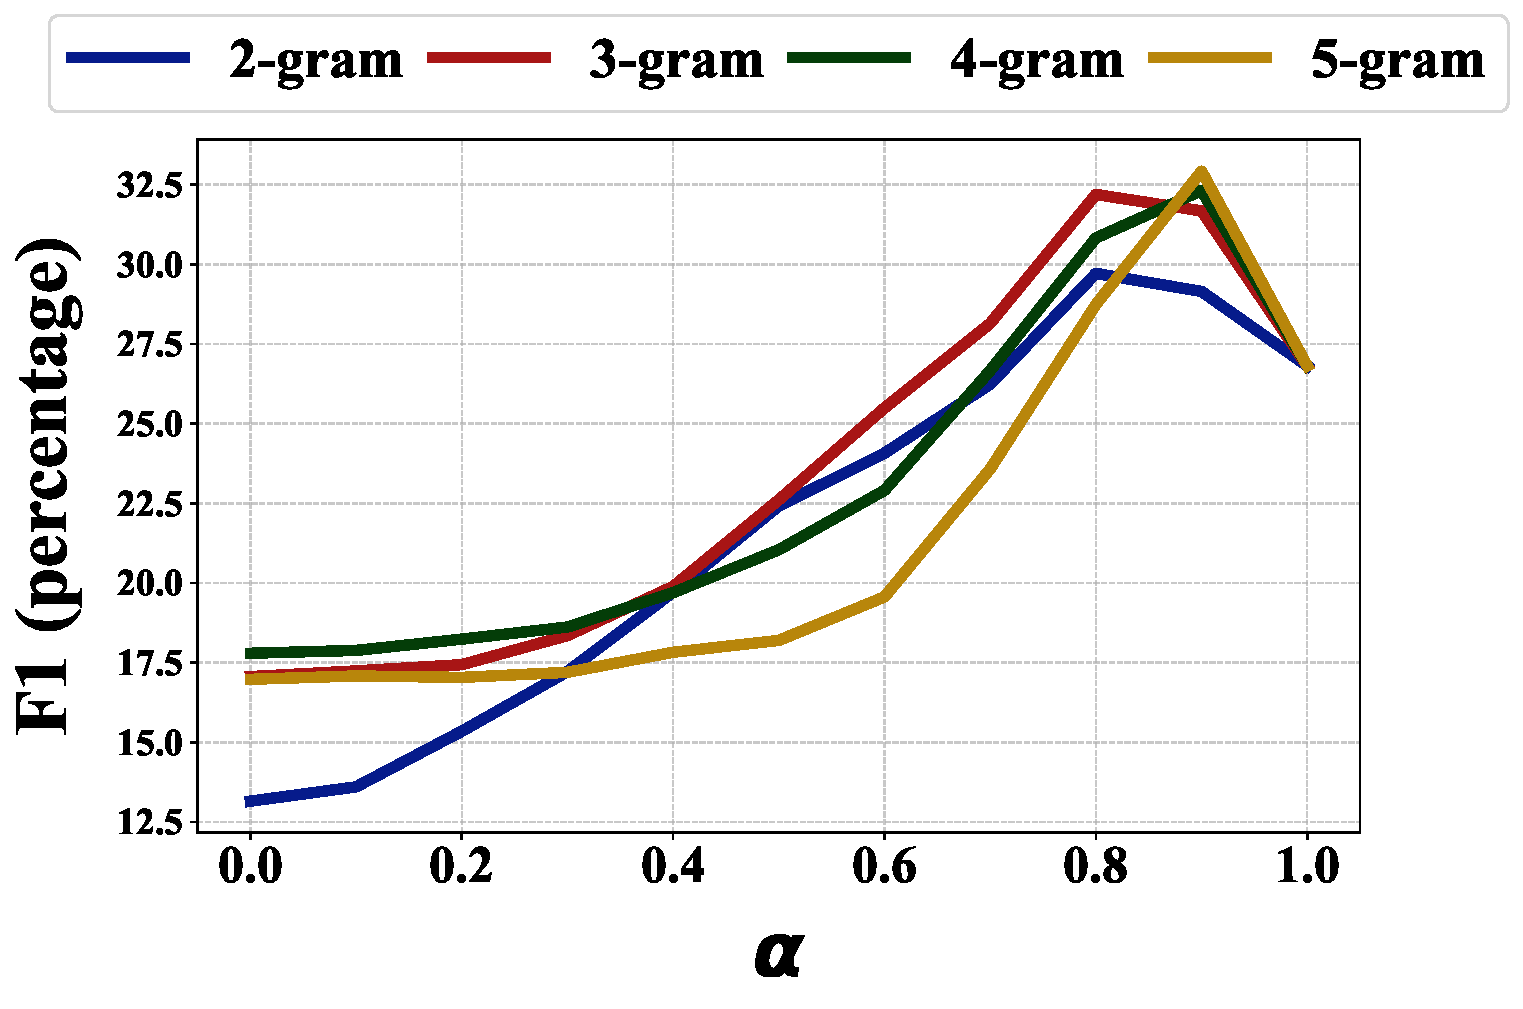
\includegraphics[width=\linewidth]{./images/ensemble-event-stat.pdf}
  \caption{LSR on Event-GNN + BM25}
  \label{fig:ensemble/eventstat}
\end{subfigure}%
\begin{subfigure}[t]{.32\textwidth}
  \centering
  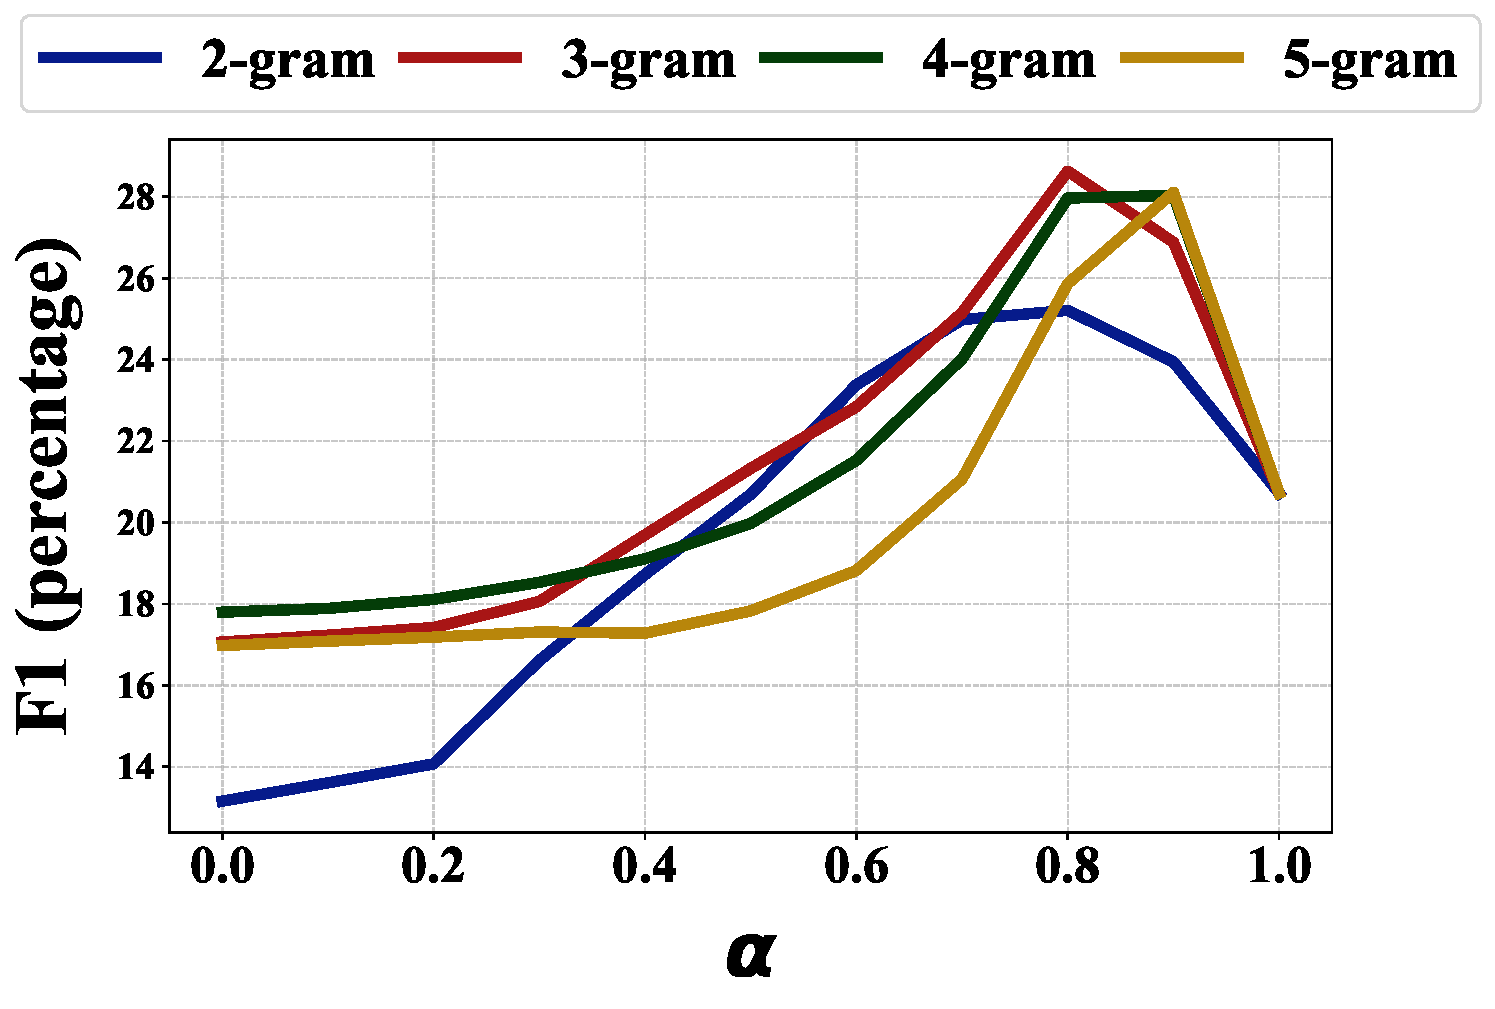
\includegraphics[width=\linewidth]{./images/ensemble-para-stat.pdf}
  \caption{LSR on Para-GNN + BM25}
  \label{fig:ensemble/parastat}
\end{subfigure}%
\begin{subfigure}[t]{.32\textwidth}
  \centering
  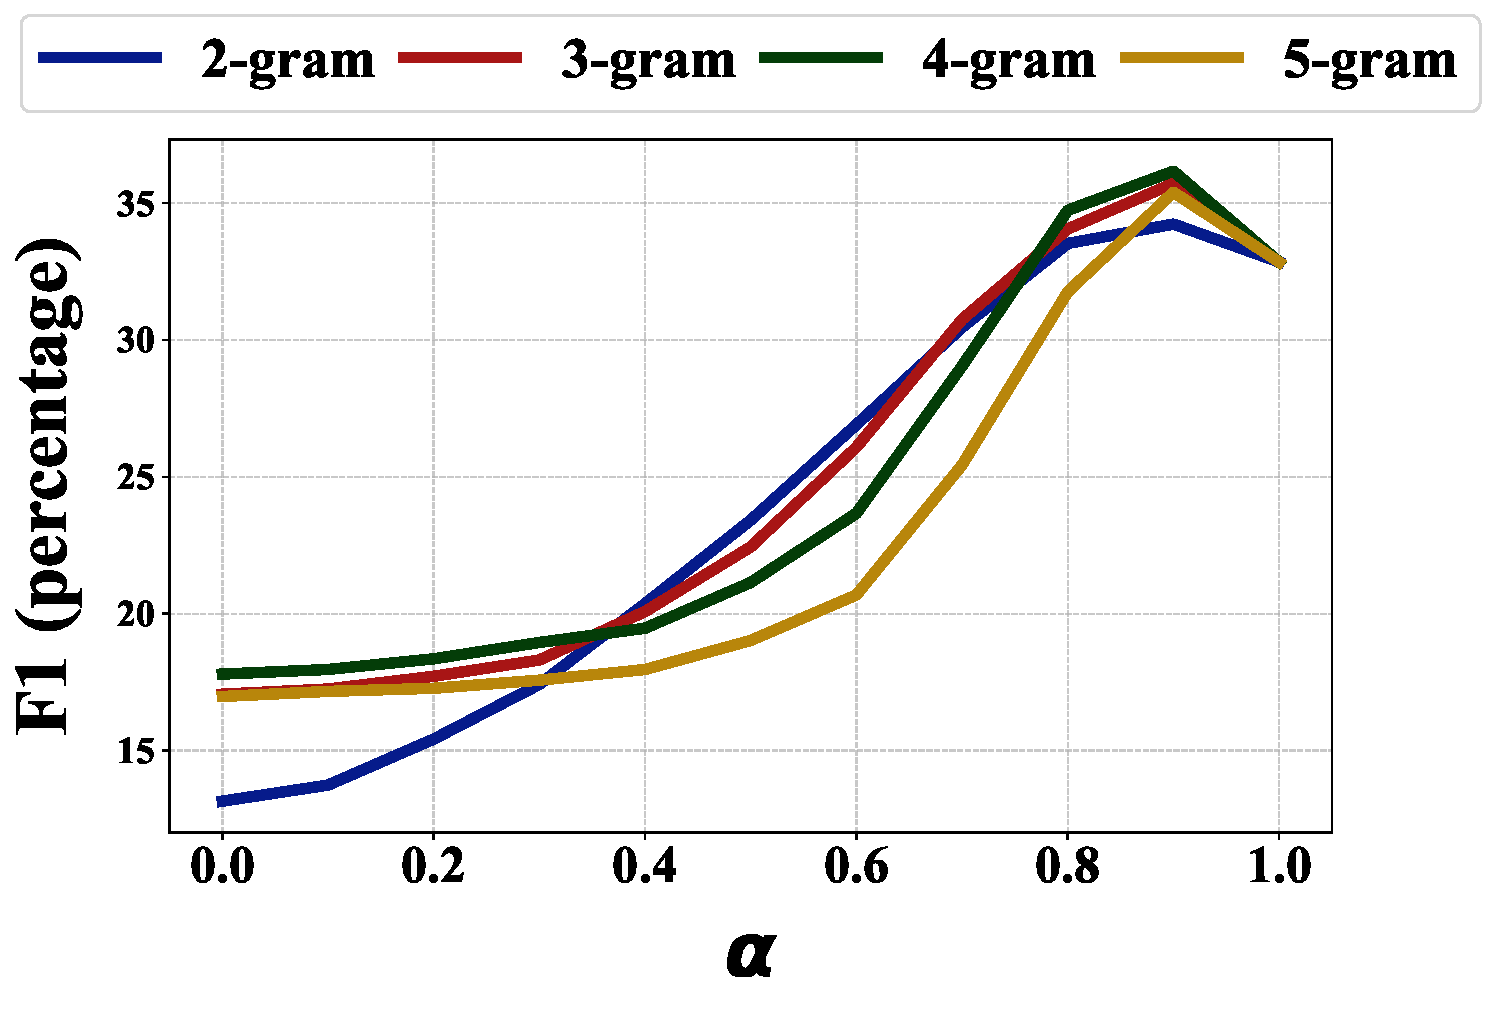
\includegraphics[width=\linewidth]{./images/ensemble-summ-stat.pdf}
  \caption{LSR on Para-GNN (summaries) + BM25}
  \label{fig:ensemble/summstat}
\end{subfigure}%
%\vspace{-4mm}
\caption{Grid Search F1(\%) of the ensemble methods for LSR task. Each figure shows the plot of performance vs. different $\alpha$ values when combining different models with BM25.} 
\label{fig:ensemble-statalpha}
%\vspace{-5mm}
\end{figure*}

\begin{figure*}
\begin{subfigure}[t]{.32\textwidth}
  \centering
  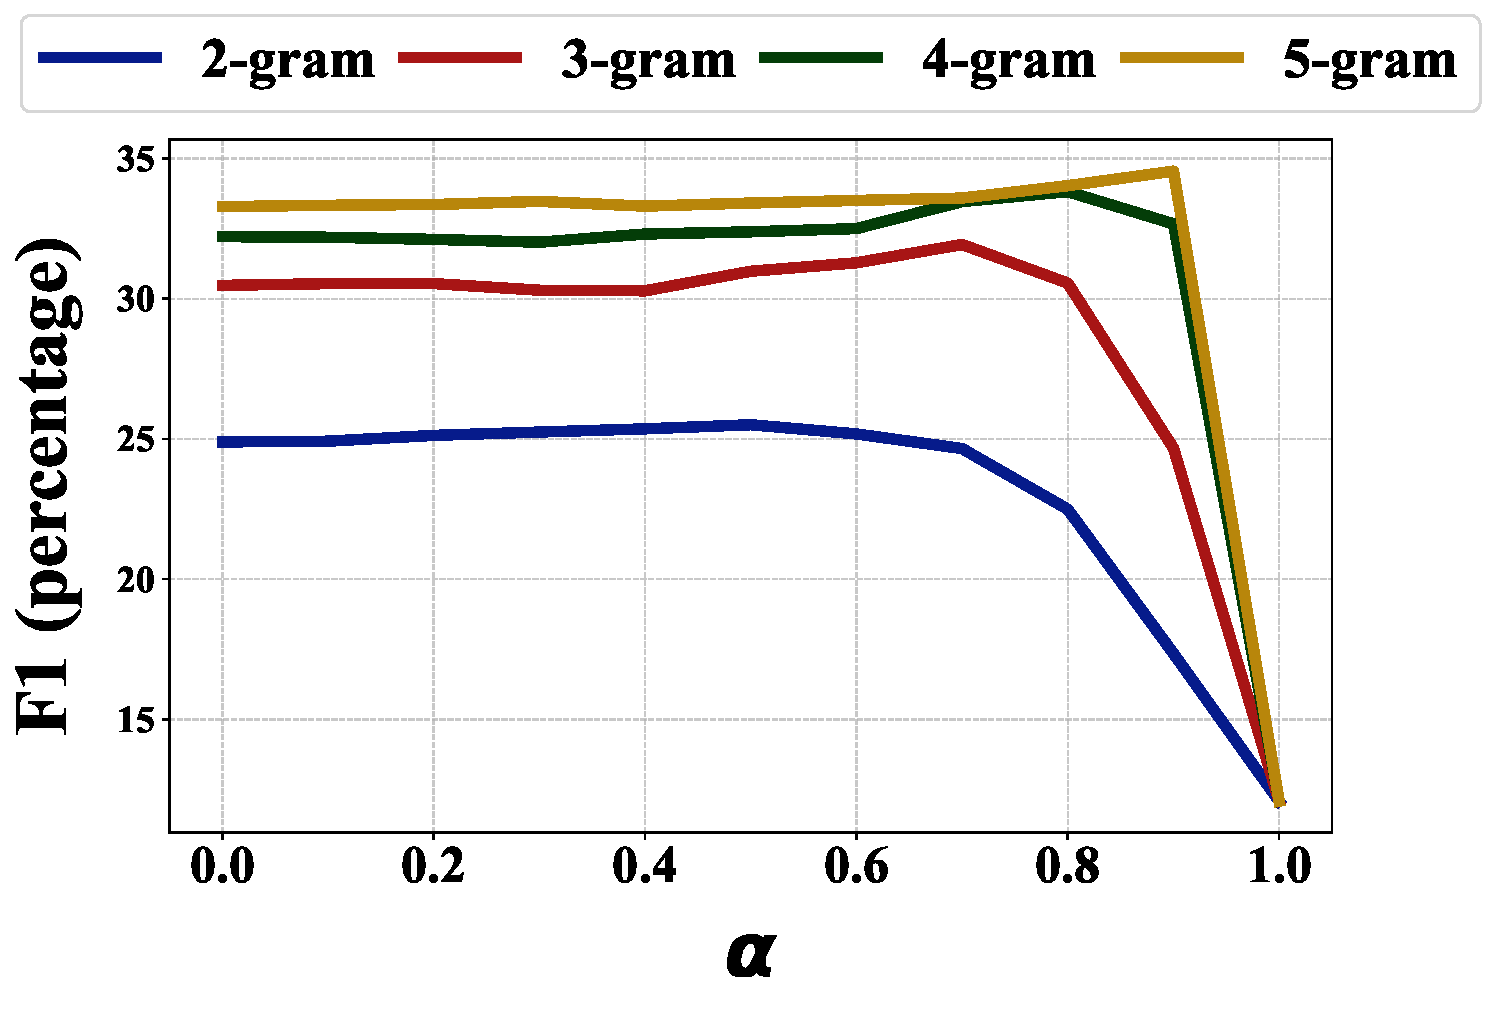
\includegraphics[width=\linewidth]{./images/ensemble-event-prec.pdf}
  \caption{PCR on Event-GNN + BM25}
  \label{fig:ensemble/eventprec}
\end{subfigure}%
\begin{subfigure}[t]{.32\textwidth}
  \centering
  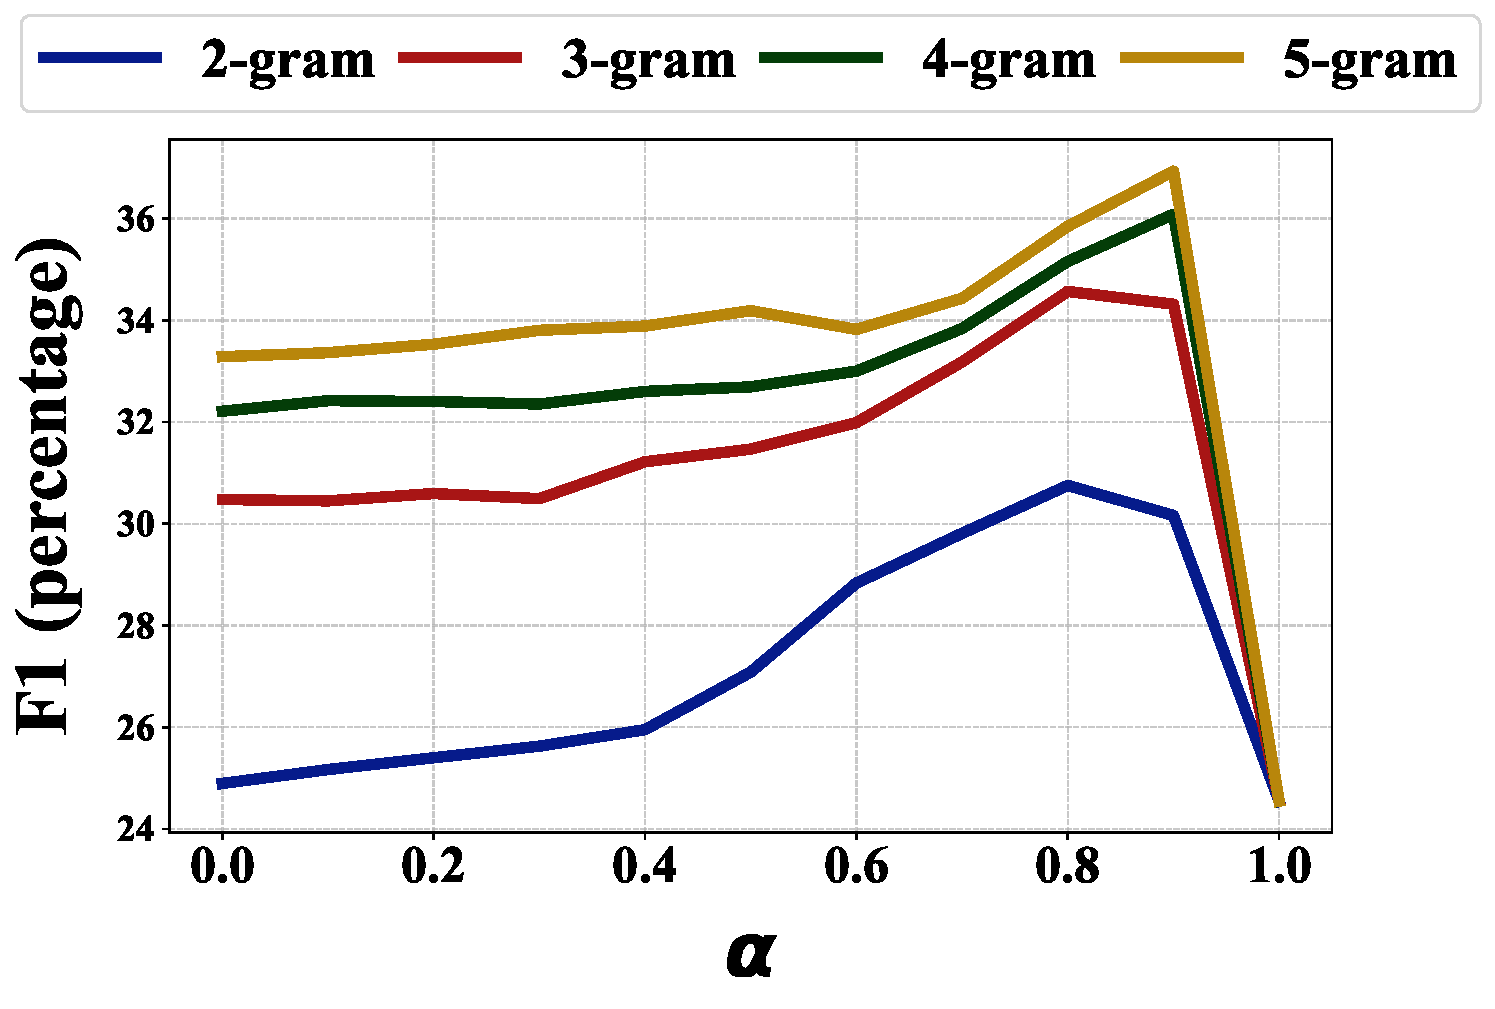
\includegraphics[width=\linewidth]{./images/ensemble-para-prec.pdf}
  \caption{PCR on Para-GNN + BM25}
  \label{fig:ensemble/paraprec}
\end{subfigure}%
\begin{subfigure}[t]{.32\textwidth}
  \centering
  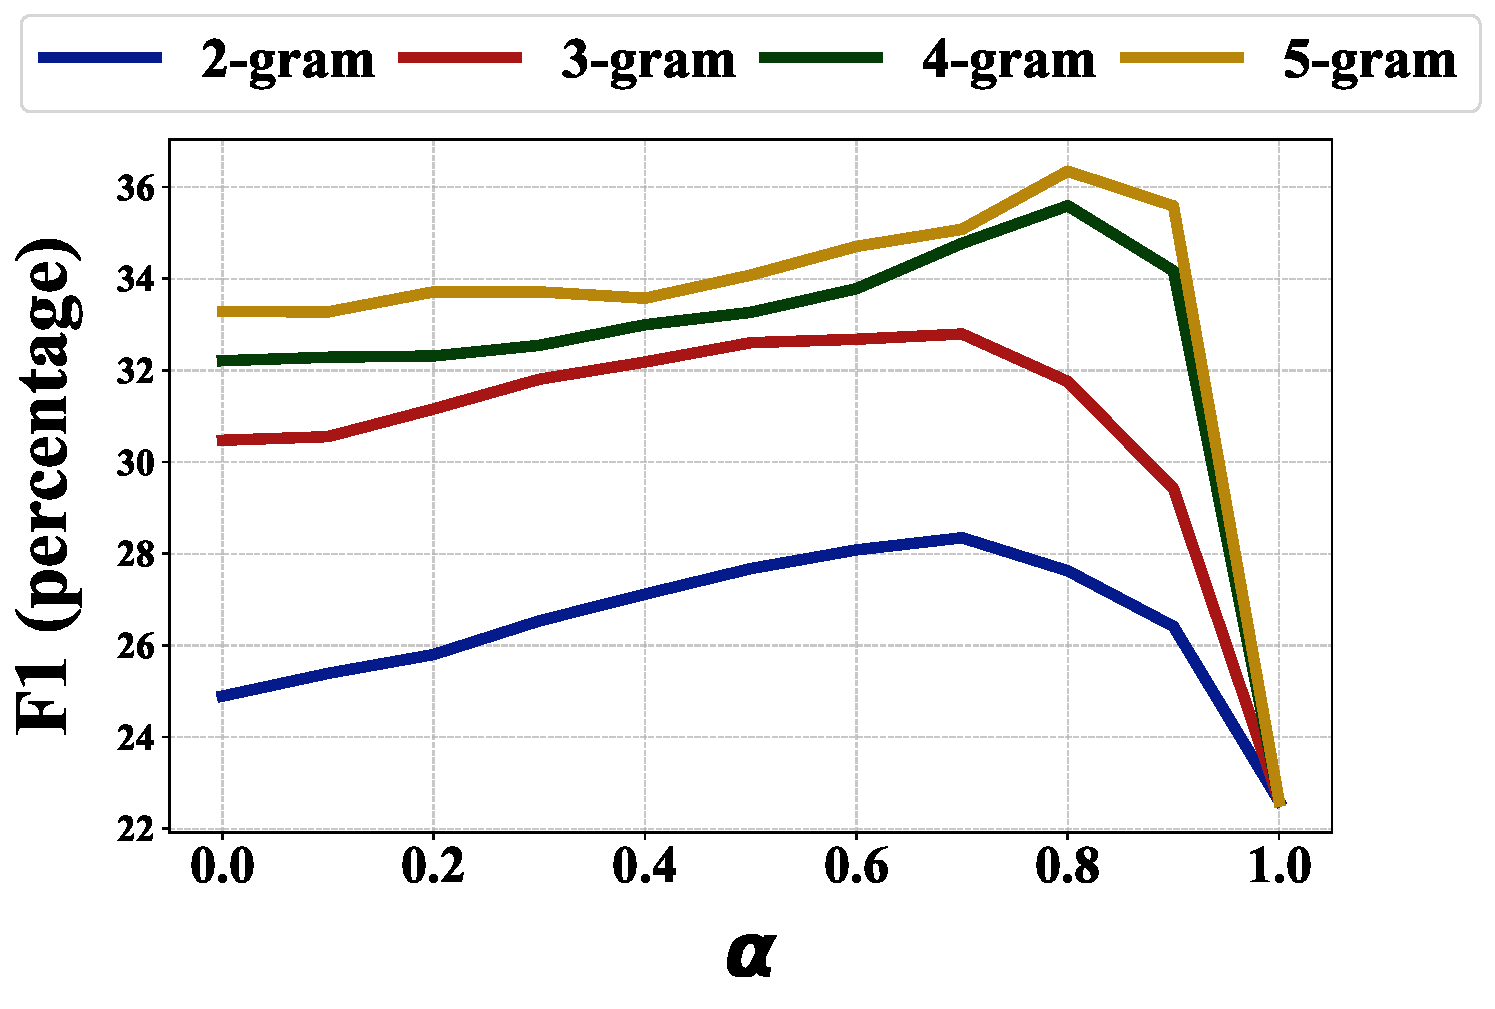
\includegraphics[width=\linewidth]{./images/ensemble-summ-prec.pdf}
  \caption{PCR on Para-GNN (summaries) + BM25}
  \label{fig:ensemble/summprec}
\end{subfigure}%
%\vspace{-4mm}
\caption{Grid Search F1(\%) of the ensemble methods for PCR task. Each figure shows the plot of performance vs. different $\alpha$ values when combining different models with BM25.} 
\label{fig:ensemble-precalpha}
%\vspace{-5mm}
\end{figure*}

\vspace{1mm}
\noindent \underline{\bf Dynamic $\alpha$ tuning:} Table~\ref{tab:dynalpha} compares the observations from grid search with the dynamic $\alpha$ method. For LSR, the learned weights (0.84–0.94) align closely with grid-search optima, confirming the \textit{semantic-heavy nature of statute retrieval}. For PCR, multi-task and transfer setups converge to values near the grid-search peaks (around 0.8), while independent fine-tuning collapses to a much lower $\alpha$ ($\sim$0.16), effectively over-weighting BM25. This explains why independent tuning lags behind, whereas transfer learning provides the most stable balance between semantic and lexical evidence. Overall, these findings reinforce the task asymmetry: \textit{LSR depends more on semantics, PCR more on lexical precision}, and ensembles are most effective when this balance is explicitly optimized.


\subsection{Statistical Significance Testing} \label{app:sigtest}
To confirm the reliability of our improvements, we performed paired $t$-tests on macro-F1 scores for the strongest ensemble and LLM-based models. We compared three ensemble variants of Para-GNN (summaries) + BM25 with dynamic $\alpha$ fine-tuning: (i)~fine-tuned separately (En-Sep), (ii)~fine-tuned in a multi-task setup (En-MT), and (iii)~fine-tuned with transfer learning (En-TL), along with the two prompting stages of GPT-4.1 re-ranking (GPT-S1 and GPT-S2). The resulting $p$-values are reported in Table~\ref{tab:sigtest}.

\begin{table}[!ht]
    \centering
    \small
    \begin{tabular}{llcc}
        \toprule
         \textbf{Method 1} & \textbf{Method 2} & \textbf{LSR $p$-val} & \textbf{PCR $p$-val} \\ 
         \midrule
         En-Sep & En-MT  & 6.8e-4  & 5e-1 \\
         En-Sep & En-TL  & 4.3e-4  & 8e-2 \\
         En-MT  & En-TL  & 8.4e-8  & 9.1e-3 \\
         En-Sep & GPT-S1 & 4.6e-32 & 6.1e-7 \\
         En-MT  & GPT-S1 & 5.3e-34 & 1.2e-10 \\
         En-TL  & GPT-S1 & 1.5e-29 & 2.2e-8 \\
         GPT-S1 & GPT-S2 & 1.8e-3  & 3.2e-3 \\
         \bottomrule
    \end{tabular}
    \caption{$p$-values from paired $t$-tests over macro-F1 scores for LSR and PCR among top-performing models.}
    \label{tab:sigtest}
\end{table}

\noindent Within the ensemble family, transfer learning (En-TL) consistently yields significant gains over both separate and multi-task fine-tuning, reinforcing its effectiveness for leveraging cross-task knowledge. More importantly, GPT-S1 significantly outperforms all ensemble variants by large margins ($p \ll 0.01$), establishing LLM re-ranking as clearly superior to traditional ensembles. Finally, the improvements of GPT-S2 over GPT-S1 are themselves statistically significant for both LSR and PCR, underscoring the benefit of incorporating cross-task dependencies in the second-stage prompt.


\begin{table*}
    \centering
    \begin{tabular}{|p{0.99\textwidth}|}
    \hline
    You are a smart and diligent Indian legal assistant with expertise in analyzing court judgments and identifying cited statutory provisions.

Context:

You will be provided with: \\
- A masked judgment: All statute names and section numbers have been replaced with placeholders like [ACT], [SECTION], etc.
- A **list of statutory sections**: Each entry includes a unique ID, and the name of the corresponding statute.

**Your Task:**

1. **Analyze the Masked Judgment:**
   - Carefully interpret the masked judgment's legal reasoning and context.

2. **Understand the Statutory List:**
   - Review the provided statute list. 

3. **Determine Cited Statutes:**
   - Identify the statute sections that are cited  in the judgment.
   - Return only the relevant **IDs** of the cited statute sections.\\
    \hline
    \end{tabular}
    \caption{Prompt used for LLM Re-ranking Statutes }
    \label{tab:qry-stat-rerank}
\end{table*}

\begin{table*}
    \centering
    \begin{tabular}{|p{0.99\textwidth}|}
    \hline
    You are a indian legal AI assistant.

Your task is to decide whether the given precedent judgment is cited by the masked query judgment. The query text may include masked placeholders like [PRECEDENT], [ACT], or [SECTION].

Return YES if the query judgment cites the precedent judgment, otherwise return NO. 

Output Format:
'Respond with exactly one word: "YES" or "NO". '
'Do not include any explanation, punctuation, or additional text.'\\
    \hline
    \end{tabular}
    \caption{Prompt used for LLM Re-ranking Precedents Stage 1 }
    \label{tab:qry-prec-rerank1}
\end{table*}

\begin{table*}
    \centering
    \begin{tabular}{|p{0.99\textwidth}|}
    \hline
    You are a indian legal AI assistant.

Your task is to decide whether the given precedent judgment is cited by the masked query judgment. The query text may include masked placeholders like [PRECEDENT], [ACT], or [SECTION]. To assist your decision, statute cited in both the query and precedent are provided.

Return YES if the query judgment cites the precedent judgment, otherwise return NO. 

Output Format:
'Respond with exactly one word: "YES" or "NO". '
'Do not include any explanation, punctuation, or additional text.'\\
    \hline
    \end{tabular}
    \caption{Prompt used for LLM Re-ranking Precedents Stage 2 }
    \label{tab:qry-prec-rerank2}
\end{table*}



% \begin{figure*}
% \begin{subfigure}[t]{.48\textwidth}
%   \centering
%   \includegraphics[width=\linewidth]{./images/freq_analysis_stats.png}
%   \caption{LSR}
%   \label{fig:freq-analysis-lsr}
% \end{subfigure}%
% \begin{subfigure}[t]{.48\textwidth}
%   \centering
%   \includegraphics[width=\linewidth]{./images/freq_analysis_precs.png}
%   \caption{PCR}
%   \label{fig:freq-analysis-pcr}
% \end{subfigure}%
% \caption{Performance in terms of F1(\%) compared to frequency of candidates. On the X-axis, the candidates are sorted from left to right according to frequency and divided into groups (most frequent group 1, most rare group 5). We compare the Ensemble model (Para-GNN + BM25) under two settings, using full documents vs. summaries. Figure~\ref{fig:freq-analysis-lsr} shows LSR performance and Figure~\ref{fig:freq-analysis-pcr} shows PCR performance.} 
% \label{fig:freq-analysis}
% %\vspace{-5mm}
% \end{figure*}

\begin{figure*}
\begin{subfigure}[t]{.5\linewidth}
  \centering
  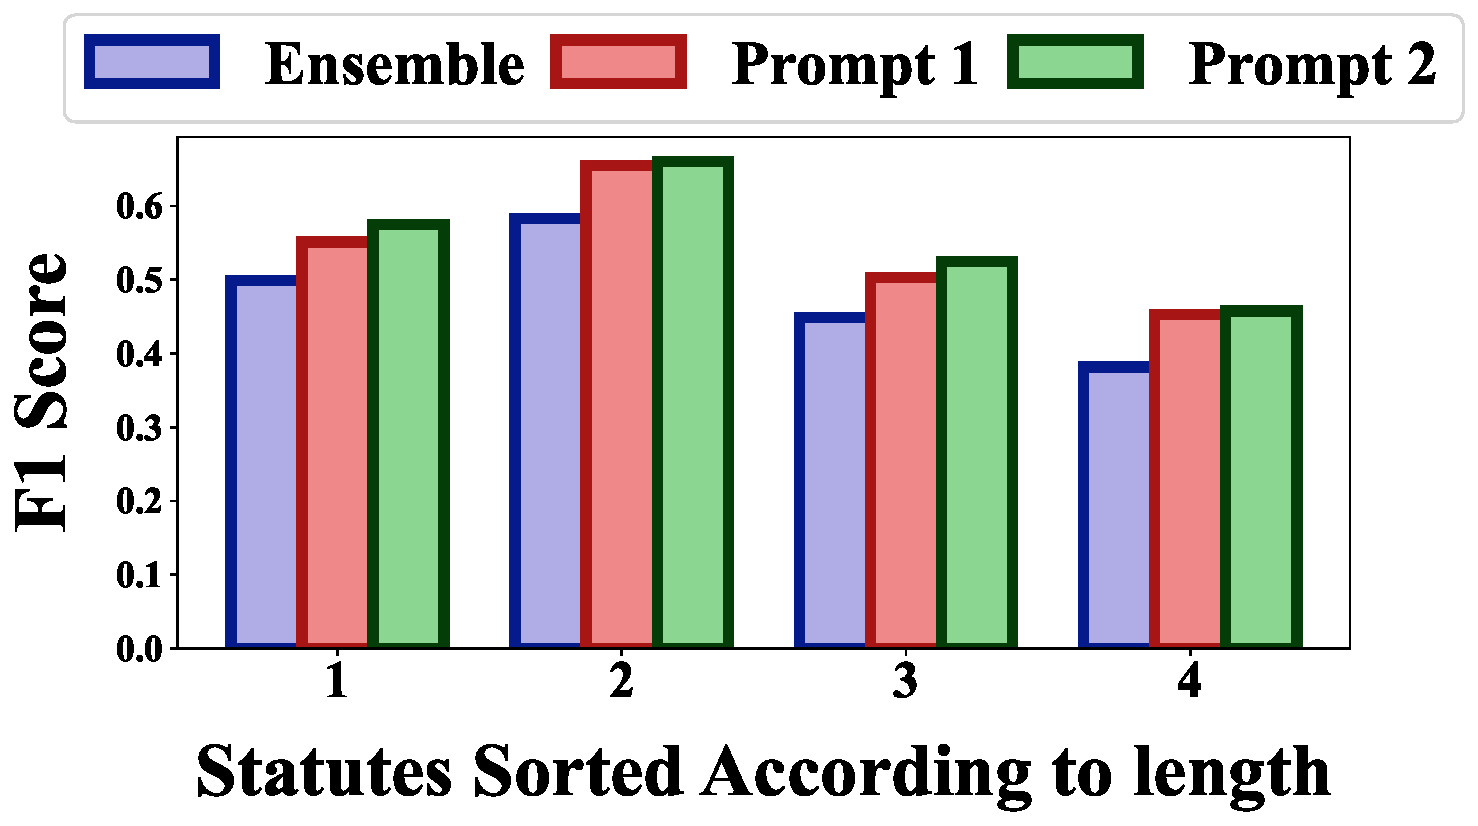
\includegraphics[width=\linewidth]{./images/llm-len-stats.pdf}
  \caption{LSR F1 vs. stat length}
  \label{fig:llm-len-stats}
\end{subfigure}%
\begin{subfigure}[t]{.5\linewidth}
  \centering
  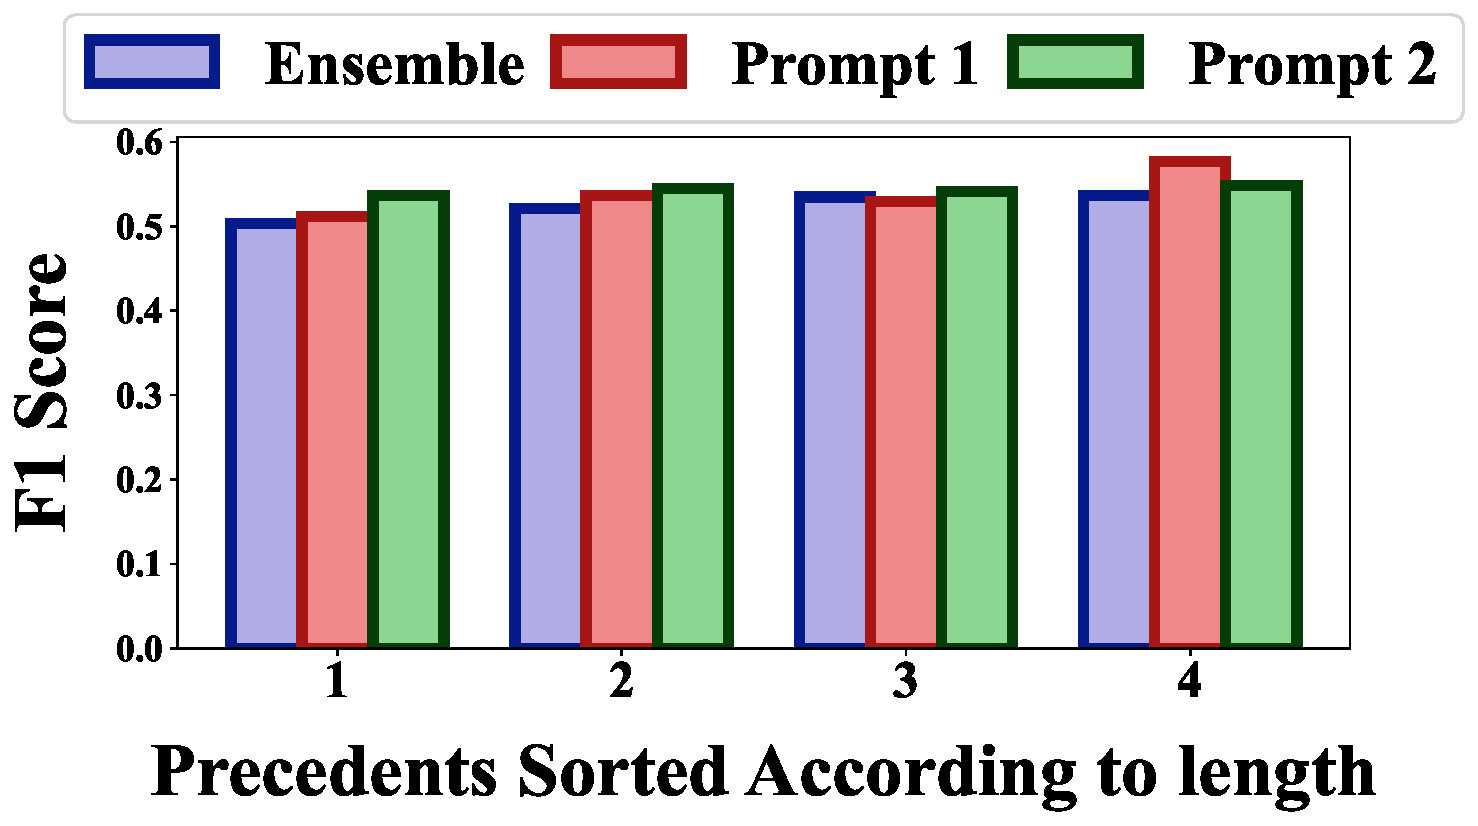
\includegraphics[width=\linewidth]{./images/llm-len-precs.pdf}
  \caption{PCR F1 vs. prec length}
  \label{fig:llm-len-precs}
\end{subfigure}%
\vspace{-2mm}
\caption{Performance in terms of F1(\%) compared to \textit{candidate} text lengths. On the X-axis, the candidates are sorted from left to right according to text length and divided into groups (shortest candidates group 1, longest candidates group 4). Figure~\ref{fig:llm-len-stats} shows LSR performance and Figure~\ref{fig:llm-len-precs} shows PCR performance with varying candidate (statute and precedent respectively) lengths.} 
\label{fig:llm-len-cands}
% \vspace{-5mm}
\end{figure*}



\begin{figure*}
\begin{subfigure}[t]{.5\linewidth}
  \centering
  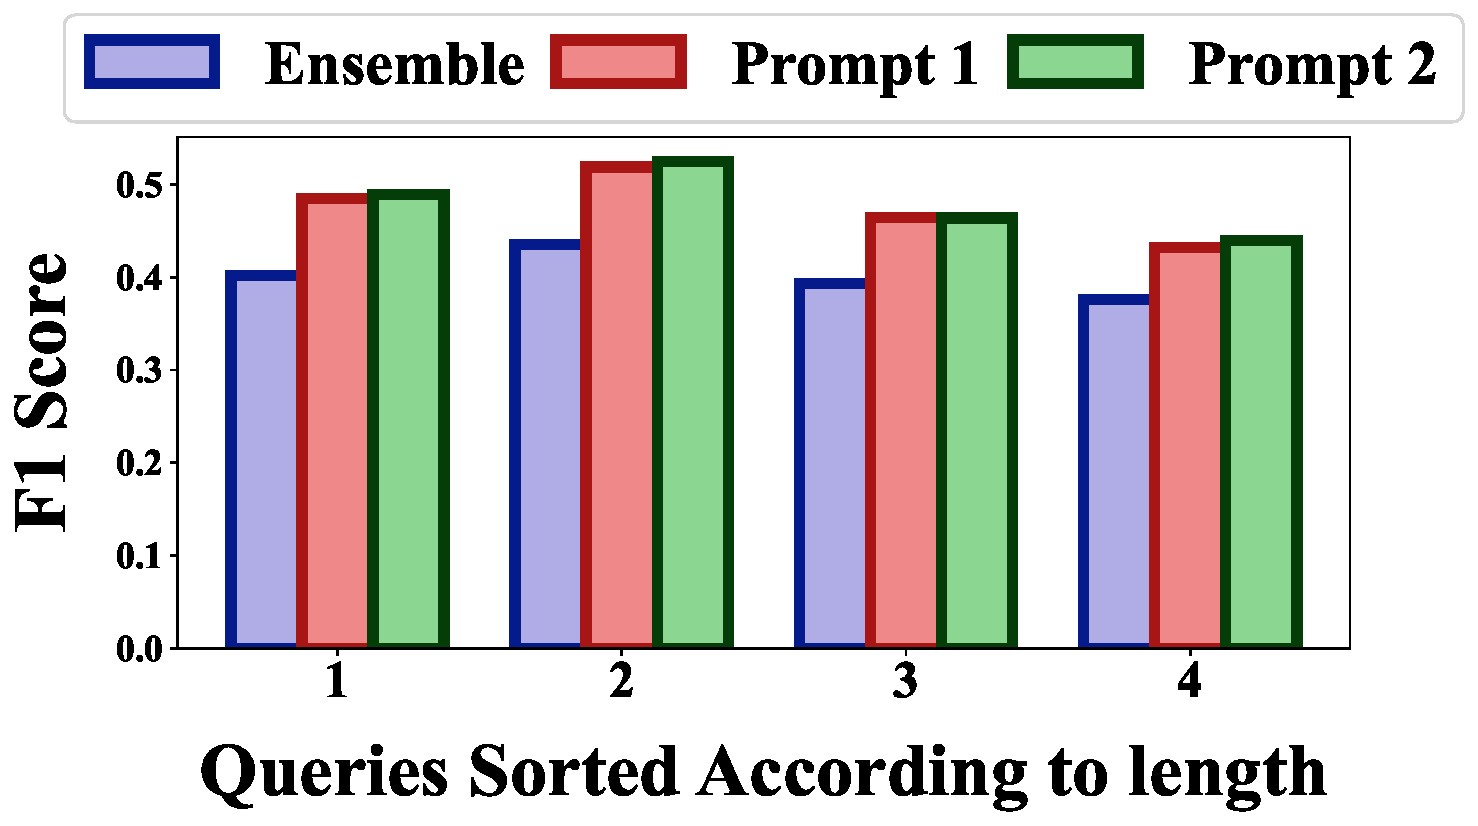
\includegraphics[width=\linewidth]{./images/llm-len-qry-lsr.pdf}
  \caption{LSR F1 vs. query length}
  \label{fig:llm-len-qry-lsr}
\end{subfigure}%
\begin{subfigure}[t]{.5\linewidth}
  \centering
  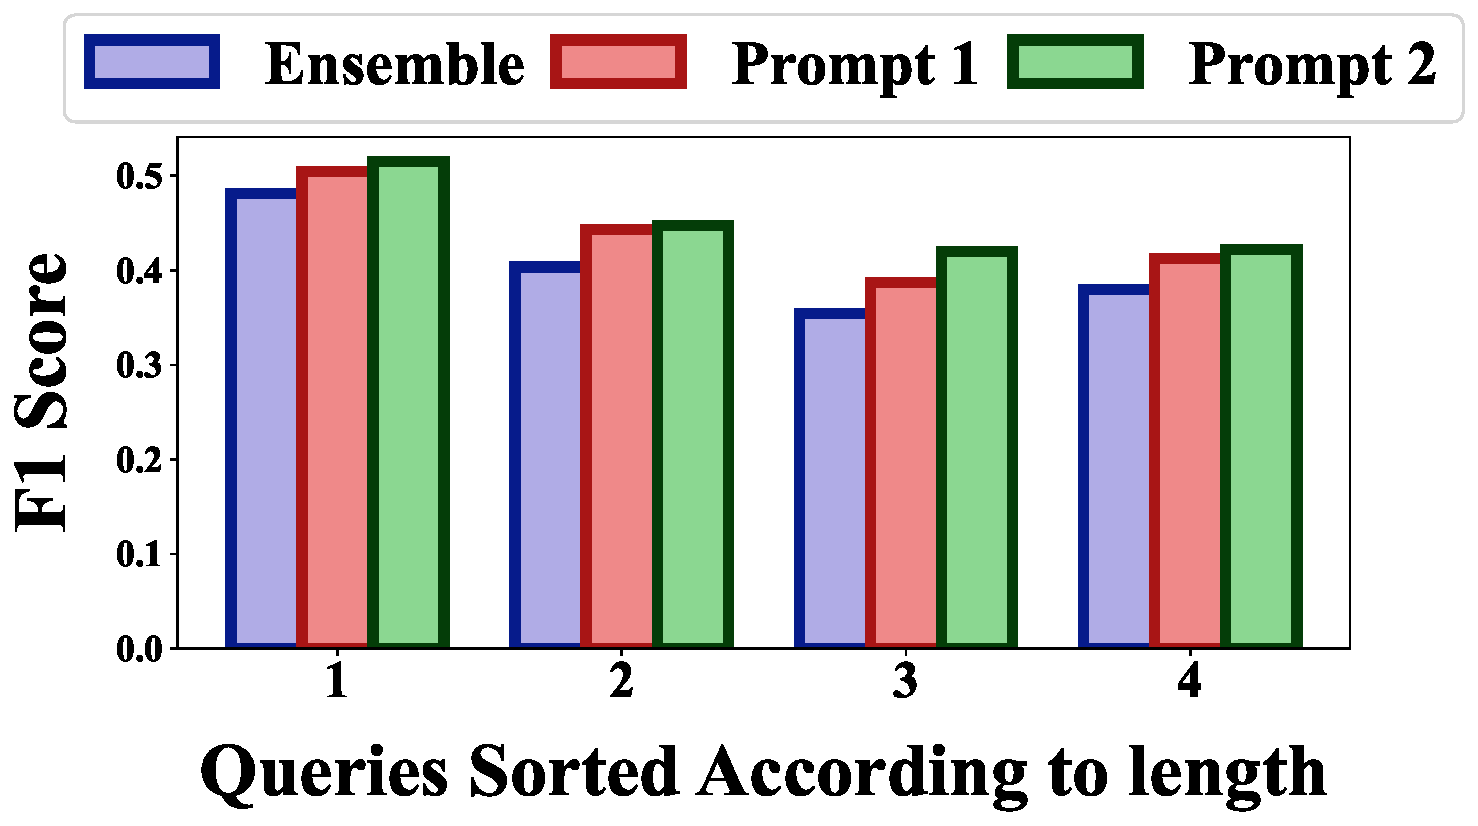
\includegraphics[width=\linewidth]{./images/llm-len-qry-pcr.pdf}
  \caption{PCR F1 vs. query length}
  \label{fig:llm-len-qry-pcr}
\end{subfigure}%
\vspace{-2mm}
\caption{Performance in terms of F1(\%) compared to \textit{query} text lengths. On the X-axis, the queries are sorted from left to right according to text length and divided into groups (shortest candidates group 1, longest candidates group 4). Figure~\ref{fig:llm-len-stats} shows LSR performance and Figure~\ref{fig:llm-len-precs} shows PCR performance with varying query lengths.} 
\label{fig:llm-len-qry}
% \vspace{-5mm}
\end{figure*}

\subsection{Analyzing the effect of candidate frequencies and text lengths} \label{app:freqlenanalysis}

% \paul{As discussed in Section~\ref{sec:expt}, the first stage LLM prompting improves upon the ensemble-based retriever across all ranges of candidate frequencies for both LSR and PCR, while the second-stage prompting mostly improves over the relatively frequent statutes (see Figure~\ref{fig:llm-freq}).}


% We also observe for all models, the fine-tuned model is able to achieve a performance close to the grid-search approach (see Table~\ref{tab:results}), which suggests that there is enough signal in the data to learn the optimal $\alpha$ ratio. On inspecting the average $\alpha$ values generated over the test set, we notice that $\alpha=0.94$ for statutes and $\alpha=0.78$ for precedents in the case of Event-GNN. For Para-GNN, the average values are $\alpha=0.85$ and $\alpha=0.82$ for statutes and precedents respectively. In case of Para-GNN with summaries, the average values are $\alpha=0.95$ and $\alpha=0.80$ for statutes and precedents respectively. Nevertheless, the ensemble models outperform the individual lexical and semantic approaches. 
We analyzed how the performance of the best models vary across candidates of different frequency ranges in \S~\ref{sec:expt} (Fig.~\ref{fig:llm-freq}). We conduct a more in-depth analysis of the effect of candidate frequency, as well as length of query and candidate texts in this Section.

\vspace{1mm}
\noindent\underline{\bf Held-out and Never-cited Candidates:} \label{app:heldout}
To analyze robustness, we study two challenging candidate types:  
(i)~\textit{held-out candidates}, i.e., statutes/precedents cited only in the test set but absent from train/dev, and  
(ii)~\textit{never-cited candidates}, i.e., candidates that are never cited in any query. 
\ilpcsr{} consists of 20 held-out statutes and 88 precedents. There are 19 never-cited statutes and 93 such precedents (Table~\ref{tab:salient-stats-ilpcsr}, App.~\ref{sec:dataset-appendix}).

\noindent {\bf Held-out candidates:} We restrict evaluation to queries that cite at least one such candidate, and compute F1 over this restricted set. Results are shown in Table~\ref{tab:heldout} (same notations for models as the above Section). For LSR, En-MT achieves the best generalization, while En-Sep lags behind. For PCR, En-Sep performs best, but differences across ensembles and GPT re-ranking are relatively small. Importantly, GPT-based re-ranking does not provide additional gains here, suggesting that ensembles remain highly competitive when generalizing to unseen candidates.

\begin{table}[!ht]
\centering
\small
\begin{tabular}{lcc}
\toprule
\textbf{Model} & \textbf{LSR F1} & \textbf{PCR F1} \\
\midrule
En-Sep  & 33.33 & 64.29 \\
En-MT   & \textbf{40.00} & 58.39 \\
En-TL   & 38.67 & 58.04 \\
GPT-S1  & 38.67 & 58.04 \\
GPT-S2  & 38.67 & 58.04 \\
\bottomrule
\end{tabular}
\caption{Performance (macro-F1, percentage) on held-out candidates.}
\label{tab:heldout}
\end{table}

\noindent {\bf Never-cited candidates:} We count the number of test queries where at least one never-cited candidate is ranked in the top-5 (Table~\ref{tab:nevercited}). A higher value indicates poorer robustness, since irrelevant candidates should not be prioritized. Here, we find that LSR is largely unaffected (almost no spurious never-cited retrievals), while PCR is more sensitive. Among ensembles, En-Sep shows the worst robustness, while En-MT and En-TL reduce false retrievals. GPT re-ranking performs comparably to the stronger ensembles, indicating that while LLMs offer gains on cited candidates, they do not exacerbate errors from never-cited ones.

\begin{table}[!ht]
\centering
\small
\begin{tabular}{lcc}
\toprule
\textbf{Model} & \textbf{LSR} & \textbf{PCR} \\
\midrule
En-Sep  & 0 & 35 \\
En-MT   & 3 & 23 \\
En-TL   & 0 & 26 \\
GPT-S1  & 1 & 24 \\
GPT-S2  & 1 & 24 \\
\bottomrule
\end{tabular}
\caption{Number of test queries where a never-cited candidate appears in top-5. Lower is better.}
\label{tab:nevercited}
\end{table}

\noindent Overall, these analyses show that while GPT-based re-ranking provides state-of-the-art gains on cited candidates, ensembles retain strong robustness on both held-out and never-cited cases. LSR models are inherently more resistant to never-cited noise, whereas PCR models require better mechanisms to handle such distractors.


%%%%%%%%%%%%%%%%%%%%%%%%%%%%%%%%%%%%%%%%%%%%%%%%%%%



% Both statutes and precedents are not uniformly distributed in the dataset, usually both these follow a long tail distribution (some candidates are cited by most queries, most other candidates are cited by few). Thus, it is interesting to analyze the performance of different models on different candidates based on their frequency of citation.
% Figure:~\ref{fig:freq-analysis} shows the performance of the Para-GNN + BM25 Ensemble (Grid Search) model with two variations, using full documents vs. summaries as input. We divide the candidate spaces into 5 equal-sized, disjoint groups based on frequency, and plot the F1 scores for each group considering only those candidates in the given group. On the query side, we only include those queries for evaluation that cite at least one candidate in the group. Naturally, groups containing frequently cited candidates are larger in size than the ones containing rare candidates.

% We observe that for statutes, the frequency plays a very crucial role, with the performance decreasing sharply across the most rare groups (Groups 4-5). The difference in performance of the model, when using summaries compared to full documents, is larger for the frequent groups, which got tuned better with the summaries. For precedents, frequency seems to play a much lesser role, with the performance on the rare groups being similar to the frequent groups. It is also interesting to note that there is a significant drop in performance for the summary-based model over Group-5 (most rare precedents). Thus, for both LSR and PCR, the summary-based methods lose their efficacy over the rare candidates.

% \noindent\textbf{Performance over held-out Candidates:}
% % As discussed in Section~\ref{sec:dataset/overview}, the \ilpcsr{} dataset contains some candidates that are not cited by any training queries but stil cited by some test queries, which can be considered as held-out candidates. There are 29 such statutes and 155 such precedents.
% \paul{[TO WRITE]}


% \begin{table}
%     \centering
%     \small
%     \setlength{\tabcolsep}{3pt}
%     \begin{tabular}{p{0.25\textwidth}cc}
%         \hline
%         \textbf{Method} & \textbf{Statutes} & \textbf{Precedents} \\ \hline
%          Event-GNN + BM25 & \textbf{37.03} & 42.88 \\
%          Para-GNN + BM25 & 28.70  & 53.18 \\
%          Para-GNN (summaries) + BM25 & \textbf{37.03}  & \textbf{54.30} \\ \hline
%     \end{tabular}
%     \caption{Performance in macro-F1@$K$ (\%) for the best ensemble methods on the zero shot candidates for \ilpcsr{}}
%     \label{tab:held-out}
% \end{table}

% Table~\ref{tab:held-out} shows the performance of the best-performing ensemble methods for the zero shot candidates. The trends for the held-out candidates follow those for the entire candidate space -- Event-GNN and Para-GNN (summaries) perform best for LSR, whereas Para-GNN (full doc) and Para-GNN (summaries) perform well for PCR. Overall, for both tasks, Para-GNN (summaries) perform the best for the held-out candidates.



%%%%%%%%%%%%%%%%%%%%%%%%%%%%%%%%%%%%
\noindent\underline{\bf Analyzing the effect of text lengths:} \label{app:lenanalysis}
% \section{Analysis with Text Lengths} \label{app:lenanalysis}
We also analyze the effect of text lengths on retrieval performance, considering both queries and candidates. For each case, we sort the documents by their token length and divide them into four groups (Group-1 containing the shortest, Group-4 containing the longest). The grouping procedure is consistent with the frequency-based analysis in \S~\ref{sec:expt}, ensuring comparability across different perspectives of candidate/query difficulty. We then evaluate performance using the same set of methods considered in \S~\ref{sec:expt}, and report macro-F1 scores. Results are shown in Fig.~\ref{fig:llm-len-cands} for candidates and Fig.~\ref{fig:llm-len-qry} for queries.  

\noindent\textbf{Varying Candidate Lengths:}  
As shown in Fig.~\ref{fig:llm-len-cands}, LLM re-ranking consistently outperforms ensembles across candidate length groups. For LSR, Stage-2 prompting provides the largest benefits for shorter and medium-length statutes, while for PCR the improvements are strongest on longer precedents, where the LLM’s ability to capture nuanced reasoning helps counteract noise in extended case texts.  

\noindent\textbf{Varying Query Lengths:}  
From Fig.~\ref{fig:llm-len-qry}, we observe that LLMs achieve substantial gains on short queries in both LSR and PCR, suggesting that they are able to compensate for missing details through contextual reasoning. While the gains on longer queries are smaller, they remain steady, ensuring that LLMs maintain superiority over ensemble methods across all groups.  

\noindent Candidate length mainly affects how models handle verbosity, with LLMs showing clear benefits on long precedents and short statutes. Query length highlights the ability of LLMs to recover missing context, especially for shorter queries. Overall, LLM re-ranking remains robust across both query and candidate length variations.

\section{Details of the Annotation Study} \label{app:annot}

As described in \S~\ref{sec:human-annotation}, we conducted an annotation study with domain experts to examine the subjectivity of legal relevance. Six senior LL.M. students (aged 24–28) carried out the annotations under the supervision of a senior faculty member, all from the WB National University of Juridical Sciences. All annotators were informed of the study’s purpose and provided explicit consent for the use of their data. The annotators (Law students) agreed to perform the annotations on pro-bono basis as they were curious about AI technology and how it can be improved for the Law domain. To further mitigate potential biases, we manually ensured that all 60 query documents were completely anonymized prior to annotation, ensuring that no demographic or sensitive information could influence the process.




%\vspace{-2mm}
\section{Experiments on COLIEE dataset} \label{sec:coliee}
%\vspace{-3mm}

\begin{table}[t]
    \centering
    %\small
    \small
    \setlength{\tabcolsep}{5pt}
    \begin{tabular}{p{0.1\textwidth}cccc}
        \toprule
        \textbf{Model} &  \multicolumn{2}{c}{\textbf{Statutes}}&  \multicolumn{2}{c}{\textbf{Precedents}}\\
         &  \ilpcsr &  \coliee &  \ilpcsr &  \coliee \\ \midrule
         BM25 (5-gram)&  16.98&  54.49&  33.29& 30.61\\
         Event-GNN&  28.67& - &  12.08& 11.48 \\
         Para-GNN&  20.72&  17.64&  24.54& 21.24\\
 Para-GNN (summaries)& & -& &18.52\\ \midrule
         Para-GNN + BM25&  28.10 & 55.96&  \textbf{36.93} & \textbf{34.52}\\
Event-GNN + BM25& 33.87& -& 34.45&34.51\\ 
 Para-GNN (summaries) + BM25& \textbf{36.17} & -& 36.35&30.25\\ \bottomrule
    \end{tabular}
    \vspace{-3mm}
    \caption{Results of the best methods on \coliee{} datasets compared to ILPCSR. All results are in terms of macro-F1@$K$. Event-GNN and summaries could not be run for \coliee{} statutes since the queries are too small for meaningful events or summaries.}
    \label{tab:coliee}
    \vspace{-6mm}
\end{table}

All our observations are drawn over the \ilpcsr{} dataset constructed in this work. We would like to verify whether the above trends are also seen on other legal datasets/jurisdictions. Since no current dataset allows the identification of both statutes and precedents together from the same query, we have to work with two separate datasets for LSR and PCR. We choose to work on the well-known COLIEE datasets~\cite{li2024coliee2024}. 
%Specifically, we use the COLIEE 2024 Task 1 (Legal Precedent Retrieval) and Task 3 (Statute Law Retrieval) datasets for the tasks of LSR and PCR respectively. 

\noindent\underline{\textbf{LSR dataset:}} We use the \texttt{COLIEE 2024 Task 3 (Statute Law Retrieval)} dataset consisting of 746 statutes from \textit{Japanese law}, and 554 queries. Note that the queries here are typically one or two sentences long, asking specifically about the laws. 
In contrast, the queries in \ilpcsr{} are real-life cases, which makes the setting more practical and challenging. 
We opted for this dataset since other existing datasets in English (ECHR2021 and ILSI) have too less statutes  (66 and 100 respectively) to be evaluated in the retrieval setup. 

\noindent \underline{\textbf{PCR dataset:}} We use the \texttt{COLIEE 2024 Task 1 (Legal Precedent Retrieval)} dataset consisting of 1,678 queries and 5,529 precedent candidates, all of which are real-life case judgments from \textit{Canadian Federal law}. This setting is similar to the queries in \ilpcsr{}. 

\noindent \underline{\textbf{Results:}}
We choose some of the methods that performed highly over the \ilpcsr{} dataset, and applied these methods on the COLIEE datasets.
The results on \coliee{} vis-a-vis \ilpcsr{} are presented in Table~\ref{tab:coliee}.
The trends on the \coliee{} dataset are almost similar to what we observed for \ilpcsr{}. 
The only difference being that, for \coliee{}, even for LSR, lexical methods such as BM25 perform the best (whereas semantic methods outperformed lexical approaches for LSR in \ilpcsr{}). 
This difference is possibly because the queries of \coliee{} are short sentences, asking directly about the statutes, whereas for \ilpcsr{} the queries are real-world long case judgments. Both for LSR and PCR, we see improvements when using an ensemble setup for \coliee{} as well. The improvement is limited in case of statutes, possibly because the performance of Para-GNN is poor. This is possibly because short queries do not have enough structure for the GNN to exploit. For precedents, where the semantic methods perform better, the improvement obtained by ensembling is high. 
This agrees with the trend we see on \ilpcsr{} (see Table~\ref{tab:coliee}). Finally, for both \ilpcsr{} and \coliee{}, in the case of PCR, we have observed that using summaries does not perform as well as using the full texts. We observe the same key findings as \ilpcsr. 




% \input{ACL-RR-Feb/submission/sections/ethics}

%\input{sections/ethics}

% \section*{References}

% \bibliography{ACL-RR-Feb/submission/sections/references}

%\bibliography{references}
% \bibliographystyle{acl-natbib}

% \clearpage
% \newpage

% \input{ACL-RR/sections/checklist}

% \clearpage
% \newpage

% \appendix
% \input{ACL-RR-Feb/submission/sections/appendix}


\end{document}

